\documentclass[degree=master,bibtype=numeric]{tongjithesis}
% 选项:
%   degree=[master|doctor], 							% 必选
%   bibtype=[numeric|authoryear], 						% 可选,数字式引用|作者-年份引用,默认为数字式(上标)引用
%   degreetype=[academic|profession|equaleducation],  	% 可选, 学术型|专业型|同等学力,默认为学术型
% 	electronic,                                 		% 可选, 电子版,(打印时删除)
%   secret,                                     		% 可选,是否保密,基本不用
%   pifootnote,                                 		% 可选,默认已打开
%   arial,                                     			% 可选,基本不用
%   arialtoc,                                  			% 可选,基本不用
%   arialtitle                                  		% 可选,默认已打开
%   注:默认已打开的选项可以使用arialtitle=false的形式关闭。

% 所有其它可能用到的包都统一放到这里了,可以根据自己的实际添加或者删除。
\usepackage{tongjiutils}
\usepackage{adjustbox}
%参考文献更新使用biblatex包, 使用gb7714-2015标准, 具体参数设置可在cls文件中搜索biblatex进行了解
%加入bib文件(老版本文件依然能够使用)
\addbibresource{ref/refs.bib}   %


\begin{document}

% 定义所有的eps文件在 figures 子目录下
\graphicspath{{figures/}}


%%% 封面部分
\frontmatter
\tongjisetup{
  %******************************
  % 注意:
  %   1. 配置里面不要出现空行
  %   2. 不需要的配置信息可以删除
  %******************************
  %
  %=====
  % 密级
  %=====
  secretlevel={保密},
  secretyear={2},
  %
  %=========
  % 中文信息
  %=========
  % 题目过长可以换行(推荐手动加入换行符,这样就可以控制换行的地方啦)。
  ctitle={基于结构与状态的电网脆弱性\\综合评估模型研究},
  cheadingtitle={基于结构与状态的电网脆弱性综合评估模型研究},    %用于页眉的标题,不要换行
  cauthor={李炅聪},
  studentnumber={1732929},
  cmajorfirst={工程},
  cmajorsecond={控制工程},
  cdepartment={电子与信息工程学院},
  csupervisor={苏永清~~~副教授},
  % 如果没有副指导老师或者校外指导老师,把{}中内容留空即可,或者直接注释掉。
  %cassosupervisor={裴刚 教授~(校外)}, % 副指导老师
  % 日期自动使用当前时间,若需手动指定,按如下方式修改:
  % cdate={\zhdigits{2018}年\zhnumber{11}月},
  % 没有基金的话就注释掉吧。
  %cfunds={(本论文由我要努力想办法撑到两行的著名国家杰出青年基金 (No.123456789) 支持)},
  %
  %=========
  % 英文信息
  %=========
  %etitle={Research on Vulnerability Analysis and \\Quantitative Evaluation of Power System \\Based on Complex Network},
  etitle={Research on Comprehensive Assessment Model \\of Power Grid Vulnerability \\Based on Structure and State},
  eauthor={Li Jiongcong},
  emajorfirst={Engineering},
  emajorsecond={Control Engineering},
  edepartment={College of Electronics and ~~~~~~~~~~~~~~~~Information Engineering},
%emajorfirst{Control Science and Engineering}
%emajorsecond{Control Theory and Control Engineering}
  % 日期自动使用当前时间,若需手动指定,按如下方式修改:
  % edate={November,\ 2018},
  %efunds={(Supported by the Natural Science Foundation of China for\\ Distinguished Young Scholars, Grant No.123456789)},
  esupervisor={A. Prof.  Su Yongqing},
  %eassosupervisor={Prof. Gang Pei (XiaoWai)}
  }

% 定义中英文摘要和关键字
\begin{cabstract}
电力系统作为维持国计民生的重要组成部分,其稳定性、可靠性及安全性至关重要。近年来,世界各地发生的多起大停电事故也引起越来越多专家学者的关注。研究表明,大多数大停电事故的发生原因是局部故障。
% 结构和状态是电网脆弱性研究的两个重要方面,电网结构的完整性是维持电网稳定运行的基础,电网状态的不稳定会导致局部故障的发生。
因此,综合评估和识别电网的脆弱环节并采取有效控制措施是避免大停电事故发生的关键。在此背景下,本文针对基于结构与状态的电网脆弱性综合评估模型展开研究,主要工作归纳如下:

% 在电力系统运行过程中,脆弱性是其固有属性,在扰动因素作用下,电网自身固有的脆弱性显现的概率大增,将对其稳定运行
% 造成威胁,因此有必要分析电力系统的脆弱性,识别电力系统的脆弱环节,科学合理地评估电网脆弱环节的脆弱性程度,对其进行结构优化和重点防护,保证电网稳定可靠运行。

本文研究了复杂网络特征参数和网络模型,验证分析电力系统的小世界性和无标度性。通过阐述复杂网络脆弱性概念得出,复杂网络的脆弱性在于其子系统的存在性,明确了本文研究的关键问题。

通过查阅各领域脆弱性相关文献,结合复杂网络脆弱性概念和电力系统脆弱性特征,得出较为清晰的电力系统脆弱性定义,并进行脆弱过程分析及数学描述。从结构和状态两个方面对系统脆弱性进行研究,
在结构方面,基于复杂网络理论建立电力系统拓扑模型,并提出结构脆弱性指标,建立了电网结构脆弱性模型;在状态方面,从节点电压稳定性、过负荷能力和电网损耗方面提出状态脆弱性指标,并建立电力
系统负荷模型,通过蒙特卡洛方法对状态脆弱性指标进行计算分析,建立了电网状态脆弱性模型。

建立电力系统脆弱性评估指标体系,分别选取反映系统脆弱性的结构和状态脆弱性指标进行分析,并对其归一化处理,采用改进熵权法和离差最大化法分别对结构脆弱性指标集和状态脆弱性指标集
进行权重分配和指标融合得到了脆弱性一级指标,进一步利用D-S证据理论对一级指标进行融合,建立了基于结构与状态的电网脆弱性综合评估模型。

最后,以$IEEE39$系统为研究对象,依据本文建立的电网脆弱性综合评估模型,
结合算例系统结构和参数分别对电力系统的结构和状态脆弱性进行分析,得到了结构脆弱性和状态脆弱性分析结果。最后,基于聚类算法和系统脆弱性综合评估结果进行脆弱节点等级评估,
根据得到的系统综合脆弱性等级评估结果,识别系统的脆弱环节。
% 针对电网结构脆弱性,本文制定了电网蓄意攻击策略,以$IEEE118$系统为研究对象,通过 MATLAB 算例仿真实验得出最优蓄意攻击策略,验证了结构脆弱性指标的合理性及重要性。
\end{cabstract}

\ckeywords{复杂网络,结构脆弱性,状态脆弱性,综合评估模型,脆弱环节识别}

\begin{eabstract}

\end{eabstract}

\ekeywords{} 
\makecover


% 目录
\tableofcontents
% 符号对照表
%\begin{denotation}
%\item[GNU] GNU's Not Unix /'gnu:/
\item[GFDL] GNU Free Documentation License
\item[GPL] GNU General Public License
\item[FSF] Free Software Foundation
\item[SMP] 对称多处理
\item[API] 应用程序编程接口
\item[$E$] 能量
\item[$m$] 质量
\item[$c$] 光速
\item[$P$] 概率
\item[$T$] 时间
\item[$v$] 速度

%\end{denotation}

%%% 以下索引按需要选择
% 插图索引
\listoffigures
% 表格索引
\listoftables
% 公式索引
% \listofequations

%%% 正文
\mainmatter
\chapter{绪论}

\section{研究背景与研究意义}
\label{sec:research_background}
随着社会的发展,人民生活和现代化水平的不断提高,导致对电能的需求越来越大,电力系统作为维持国计民生的重要组成部分,其稳定运行、经济性、可靠性以及安全性越来越重要。
近年来,随着电力系统规模的不断扩大和电力系统复杂性的逐步增加,使得电力系统各元件之间的关联越来越紧密。电力系统在促进社会发展和人民生活水平提高的同时,由于某一局
部故障而导致电网的连锁性崩溃,甚至导致大停电事故的例子屡见不鲜,从这方面来讲,这些电网故障不仅带来巨大的经济损失,还将严重影响社会经济的发展和人民的生活水平的提高。

自进入21世纪后,全球各地发生了很多大面积电网瘫痪事故。在国内,近年来,对社会经济和人民生活影响最大电网故障要数2008年南方特大雪灾导致的全国大范围停电事故了,这一年
我国遭遇了50年一遇的冰雪灾害,由于暴雪、冻雨导致华南地区、华中和华北部分地区输变电线路出现大范围断线倒塔,造成大范围停电限电,严重影响了电网安全运行,有地区甚至断
水断电十余天,引发交通运输、物资调度、等方面的连锁反应,严重影响了人们的日常生活,影响人数达2亿人。据调查统计,此次灾害导致停运电力线路37606条,停运的变电站共2027
座,111--500~kV线路倒塌8165座,给南方地区造成了巨大的经济损失。
在国外,2018年3月21日,巴西电网发生大面积停电事故,涉及巴西北部与东北部14个州,其中受影响最为严重的是贝里奥格兰德州、帕拉伊巴州和马拉尼昂州。在此次停点事故中,北部
和东北部电网与主网裂解,最终损失负荷21735~MW,相当于巴西互联电网停电前负荷的27\%,全国约四分之一的用户断电。事故原因为巴西欣古换流站交流测500~kV断路器故障\cite{refs1}。
此外,近期发生的“3.7”委内瑞拉停电事故,委内瑞拉政府称电力系统遭到三个阶段的攻击,分别是网络、电磁和人为破坏的攻击,其攻击的方式都是使电力系统的中枢节点,从而引起电力系
统连锁反应,导致委内瑞拉23个州中,一度有20个州全面停电,造成大规模交通拥堵,学校、医院、工厂、机场等都受到严重影响,给人们带来巨大恐慌。

在世界范围内,电力系统大停电事故发生的频率虽不高,但已逐渐得到人们的重视。国内外学者开始研究停电事故的原因以及如何降低其发生的概率,于是电网脆弱性的研究也越来越成为
专家学者研究的热门领域。从大多数停电事故的原因可以看出:电网大面积瘫痪之初,都是某一元件的局部故障所引起的,由于电网的级联特性,电网的故障范围不断扩大,最终导致大面
积停电事故发生。导致元件局部故障因素有很多,比如外部环境的变化、网络攻击以及人为操作等,电力系统在运行过程中,脆弱性是电力系统固有的属性,当这些扰动因素作用于电力系
统时,电力系统的脆弱性显现的概率会大增,电力系统自身潜在的脆弱性会对其安全可靠运行造成严重威胁,因此有必要对电力系统进行脆弱性分析,研究其脆弱性指标,并建立量化评估
模型,进一步识别出系统的脆弱环节,为电力系统设计和维护人员提供可靠安全的预防方案,从而降低电力系统发生故障的概率。
\section{国内外研究现状}
\label{sec:research_presentSituation}

\subsection{脆弱性研究起源及现状}
\label{sec:origin}
脆弱性,这一概念在医学领域中被最早提出,在流行病学\cite{refs2,refs3}中,研究的是某些地区更容易发生流行病,或人体的哪些部位更容易被细菌或病毒感染。
在心脑器官领域中,研究的是不同药物或治疗方案对心脑血管以及其他脏器的耐受程度\cite{refs4,refs5}。20世纪70年代后,专家学者开始将脆弱性概念用于生态系统领域\cite{refs6,refs7}。
80年代后,脆弱性逐步扩展到自然灾害和全球气候变化中,并逐步在可持续发展的研究中频繁出现,进入21世纪,脆弱性的研究逐渐延伸到社会经济体系、计算机网络、工业控制系统以及
电力系统领域。

“脆弱性”概念早在20世纪60年代就已提出,在很长时间一直用于环境科学,医学以及人文科学。脆弱性领域的研究覆盖多个学科,不同领域对脆弱性现象的研究侧重点不同,到目前为止,还没有
一个公认的脆弱性概念。20世纪70年代起,一些生态环境研究者开始研究生态领域的脆弱性现象,学者M.Pacifici分析研究了气候变化对生态系统中物种多样性带来的脆弱性影响,他对脆弱性的
理解是气候变化对生物种类的影响程度,并建立了三种评估气候脆弱性的模型\cite{refs8}。在1991年,美国和前苏联建立了生态脆弱性的评价方法与评价因子,对生态脆弱性的起因、脆弱程度
以及相关的补偿机制开展了大量实验研究\cite{refs9}。在经济学领域中,经济学家认为脆弱性是对于未知情况的可能性或不确定性,具体指的是系统受到不利因素或者受到损害的可能性或不确
定性\cite{refs10,refs11}。金融学家Minsky在1982年提出的“金融脆弱性假说”为金融脆弱性理论研究提供了分析框架\cite{refs12},与之后Diamond和Dybvig的“预期自致型理论”和“安全边
界说”\cite{refs13},这三个理论分别从投机、信心、银行资产质量等方面阐述了银行脆弱性生成机理。直到1990年以后,脆弱性概念逐渐进入工程研究领域,在控制科学与工程领域,1997年,
LH.Keel和SP.Bhattachacharyya对$H_{2}$、$H_{\infty}$以及$l$等鲁棒控制器组成的控制系统进行研究,发现优化后的闭环控制系统在特定外部扰动的作用下极易产生不稳定的状态,其稳定
裕度指标很差,于是采用了“脆弱性”概念来描述控制系统这种隐形特性\cite{refs14}。在网络安全领域中,国内外专家们对网络脆弱性评估技术进行了深入的理论研究和实际应用,提出了一系列
的评估模型,主要有定性、定量、基于规则和基于模型等评估方法,还有后来发展的动态和分布式评估方法\cite{refs15,refs16}。

在国内,中国学者对脆弱性理论的研究相较于国外起步较晚,脆弱性概念最早出现在计算机网络领域\cite{refs17},在全球化趋势下,中国社会经济快速发展,各个领域的矛盾和摩擦层出不穷,
中国学者对脆弱性的研究领域不断扩展,研究方法不断深入,在生态系统\cite{refs18,refs19}、气候变化\cite{refs20,refs21}、金融机构\cite{refs22,refs23,refs24}、信息安全
\cite{refs25,refs26}、交通运输\cite{refs27,refs28}等方面进行了广泛的研究。在脆弱性理论和研究方法上,也不断进行研究和探索,目前国内学者普遍认为脆弱性是系统本身固有的一种
属性,由于系统本身对扰动有一定的敏感性,不同的系统对扰动作用后的恢复能力不同,只有在内部或外部扰动作用下,系统脆弱性才可能显现。在研究方法上,主要以研究脆弱性指标\cite{refs29},
脆弱性指标融合方法\cite{refs30},脆弱性评估模型为主。近年来,在电力系统研究领域,复杂网络理论\cite{refs31}受到了越来越多学者的重视,并以此为基础进行电力系统建模以及脆弱性
指标的研究,从而进一步对电力系统结构和状态两方面进行脆弱性的综合分析。


\subsection{电力系统脆弱性研究综述}
\label{sec:presentPowerSys}
电力系统是有发电厂、送变电线路、供配电所和用电等环节组成的电能生产与消费系统。电力系统脆弱性是近年来针对电力系统安全性和可靠性提出的一个新概念,目前还没有公认的定义和统一的
分析标准。但从已有的参考文献看,电力系统脆弱性是用来描述系统在正常运行情况或各种随机因素的作用下,系统承受干扰或故障的能力及系统不能维持正常运行的可能趋势及其影响\cite{refs32}。
有学者将引起系统脆弱性显现的不确定因素成为脆弱源,比如气候变化、地理、认为破坏等因素,将系统内部某些易发生故障的环节称为系统脆弱点。

通过查阅大量的参考文献后,对电力系统脆弱性的研究内容分为以下四类:
\begin{itemize}
  \item 电力系统脆弱性研究理论与方法
  \item 电力系统脆弱性评价指标的研究
  \item 针对电力系统评价指标建立系统评估模型
  \item 根据脆弱性评估结果提出相应的安全管理机制与应对策略 
\end{itemize}

在电力系统脆弱性理论研究方面,复杂网络是把一个复杂系统抽象为网络,将复杂系统内的元件视为网络的节点,将元件之间的联系视为连接网络中各个元件的边,由此建立复杂网络的模型。在此模型
基础上,从复杂网络的拓扑模型出发,运用图论、统计学理论对整个复杂网络进行局部、全局的研究,经过二十多年的发展,复杂网络的建模和分析方法,可用于描述系统内各个元件的相互关联以及系
统的整体描述,并且该理论和其研究方法已越来越多应用于各个领域,比如社会关系网络\cite{refs33}、交通运输网络\cite{refs34,refs35,refs36}、航空海运网络\cite{refs38,refs39}、电力
系统网络\cite{refs40,refs41}等,大多数复杂网络的复杂性的特征为:网络规模庞大、连接结构的复杂性、节点的复杂性、网络时空演化过程复杂、多重复杂性融合等,电力系统作为最复杂、最广泛
的人造技术网络,具有以上复杂网络的特性。加之复杂网络理论在二十多年的发展中,成为电力系统研究领域中最具权威性的理论。

在电力系统脆弱性评价指标研究方面,通过参考大量文献研究后,主要分为两个方面进行研究分析,从电力系统拓扑结构来讲,主要基于复杂网络理论来进行研究,复杂网络的结构评价指标有:平均路径
长度、节点度、聚类系数、介数、网络冗余、网络结构熵、系统全局效能等。通过复杂网络理论进行建模,在复杂网络的特征参数的基础上,进行电力系统结构脆弱性指标的研究。从电力系统运行状态来讲,
主要是基于裕度、灵敏度、能量函数这三个方面进行指标研究,裕度法主要是通过比较电力系统当前运行状态点与临界点的裕度指标来评估节点的脆弱性\cite{refs42,refs43,refs44};灵敏度法是采用
灵敏度分析法通过改变某一变量研究其对系统变量的影响程度来评估系统的状态脆弱性\cite{refs45,refs46};能量函数法是通过能量函数表达式对支路或节点的状态脆弱性进行评估,其考虑的是系统的
暂态脆弱性\cite{refs47,refs48,refs49}。以上三种方法可由能量裕度、节点电压、系统频率、节点功率以及发电机功角等为基础指标进行进一步研究分析。

在电力系统评估量化研究方面,基于复杂网络分析评估法、基于暂稳脆弱性评估法和基于概率风险的脆弱性评估法是三类常用的方法。基于复杂网络分析评估法是以复杂网络为基础,从网络拓扑结构分析连锁
故障的传播机理\cite{refs50,refs51,refs52};基于暂稳脆弱性评估法主要研究的是电力系统在暂态过程中是否能够保持在稳定的状态,此类方法主要包括基于暂态能量函数的脆弱性评估\cite{refs53}
和基于关键割集法的脆弱性评估方法\cite{refs54};基于概率风险的脆弱性评估法中有确定性评估法\cite{refs55}、概率性评估法\cite{refs56}、风险评估法\cite{refs57},此外基于蒙特卡洛法进行
脆弱性评估\cite{refs58}也是比较常用的,这些方法大多采用的是概率统计的方法对系统进行脆弱性评估。在系统脆弱性指标融合方法的研究中,可以参考与改进的主要领域在多属性决策方面,主要分为
主观、客观和组合赋权三个方面,主观评价方法有层次分析法、模糊层次分析法、专家调查法和环比评分法等;客观评价法主要有离差最大化法、熵信息法、基于方案满意度法、基于方案贴进度法等;组合赋权
法是指将不同赋权法所得到的权重系数按照一定的方法进行组合\cite{refs59}。

通过建立电力系统的评估模型,可根据融合指标值对电力系统的节点或支路的脆弱性等级进行划分,根据节点或支路的脆弱性等级,对电力系统采取相应的安全管理机制与应对策略,从而减低电网连锁故障发生
的概率,保障用电安全。



\section{研究内容与研究路线}
\label{sec:research_curise}

\subsection{待解决的问题}
\label{sec:research_problem}
对于电力系统的脆弱性分析与量化评估的研究至今依然存在很多待解决的问题,如:
\begin{enumerate}[(1)]
  \item 脆弱性概念虽然很早就已经提出,但对于电力系统的脆弱性描述和定义尚不清晰,缺乏全面性;
  \item 电力系统中的脆弱性研究的研究理论与方法虽然比较权威和可行,但是在脆弱性指标研究方面,大多数论文只从单一方面进行研究分析,评价指标缺乏全面性;
  \item 在指标融合方法上,虽然各个研究领域的指标融合方法各有千秋,但对于在电力系统的指标融合方面的考虑不够合理全面;
  \item 对于电力系统脆弱性量化分析与研究,脆弱性量化评估模型的相关研究未形成严格的理论体系。
 \end{enumerate}

\subsection{研究内容与章节划分}
\label{sec:contendAndIdea}
本文针对电力系统脆弱性分析与量化评估研究中待解决的问题,在研究了复杂网络与电力系统之间的关联基础上,给出了较为科学合理的电力系统脆弱性定义。并进一步对电力系统从结构和状态两个方面分别
给出结构脆弱性和状态脆弱性的定义与数学描述,使得电力系统的脆弱性概念更为全面。根据结构脆弱性和状态脆弱性的理论研究进行脆弱性指标选取,从而建立系统脆弱性综合评估指标集。分别对一级脆弱
性指标和二级脆弱性指标进行量化、权重分配、指标融合形成了电力系统脆弱性量化评估模型。并且以$IEEE39$系统数据为例进行电力系统的脆弱性分析与量化,识别系统的脆弱环节。本文的章节安排如下:

第~1~章~:查阅国内外“复杂网络”、“脆弱性分析”等相关领域研究文献与论文,对脆弱性概念的起源与发展以及脆弱性在电力系统的研究现状做了详细的调研与综述,为后续研究电力系统脆弱性与量化分析方
法提供必要的理论依据。在明确研究方向和理论依据的基础上,科学提炼出待解决的问题,确定研究方法、目标和技术路线。

第~2~章~:研究分析复杂网络理论的相关概念,对复杂网络的定义与数学描述进行分析,以此为基础建立电网模型。在研究复杂网络的基本特征参数的同时,为后续第三章提出结构脆弱性指标提供理论依据。
在分析复杂网络定义与特性的基础上,进一步分析研究复杂网络的脆性理论,分析整个复杂系统的脆弱性指标,为后续第五章的电力系统结构脆弱性仿真实验分析打下基础。为了验证电力系统的网络特性,
本章还研究分析了复杂网络的小世界模型和无标度模型。

第~3~章~:通过研究分析电力系统稳定性、可靠性、鲁棒性之间的区别与联系,得出有电力系统脆弱性的本质以及脆弱过程,在此基础上给出电力系统脆弱性的数学描述;分别从电力系统结构和状态两个方面
对脆弱性的理论分析方法进行研究,并提出脆弱性指标。从结构脆弱性角度来看,侧重于系统保持其结构完整性的能力,研究系统在扰动作用下受影响的程度,为后续的攻击策略及电网结构脆弱性仿真实验打
下基础。而在状态脆弱性角度来看,专注于在系统运行过程中,系统的抗干扰能力,建立了负荷模型,结合蒙特卡洛模拟方法,并以此作为状态脆弱性仿真分析的基础。

第~4~章~:针对结构脆弱性与状态脆弱性,分别根据各自脆弱性的定义与特征选取能够反映其脆弱现象的评价指标,结合并改进客观评价法及多指标融合法,建立了电力系统脆弱性量化评估的数学模型。解决
了系统脆弱性现象难以量化的问题,为后续量化评估电力系统脆弱性问题提供了理论参考。

第~5~章~:以$IEEE118$电力系统为例,在系统模型建立的基础上,研究不同攻击策略对电网拓扑结构完整性及系统性能的影响程度;在电力系统状态脆弱性方面,以$IEEE39$电力系统为例,分析不同指标对
系统状态的影响,采用多指标融合方法得到状态脆弱性综合指标,并和结构脆弱性综合进行对比,进一步量化分析电力系统节点的脆弱程度,最后得到系统的综合脆弱性模型,基于脆弱性量化评估模型对电力
系统节点脆弱性进行等级划分,得出脆弱性评估结果为后续安全管理机制与应对策略提供了理论依据。

第~6~章~:总结本文的研究工作,对本文中电力系统脆弱性分析与量化数学模型的优点和不足进行了详细的阐述,并为后续研究工作提出了若干点建议与展望。

通过以上的研究工作,完成电力系统脆弱性分析与量化评估的理论研究及实验验证与分析,具体的技术路线图如下所示。
\begin{figure}[H] % use float package if you want it here
  \centering
  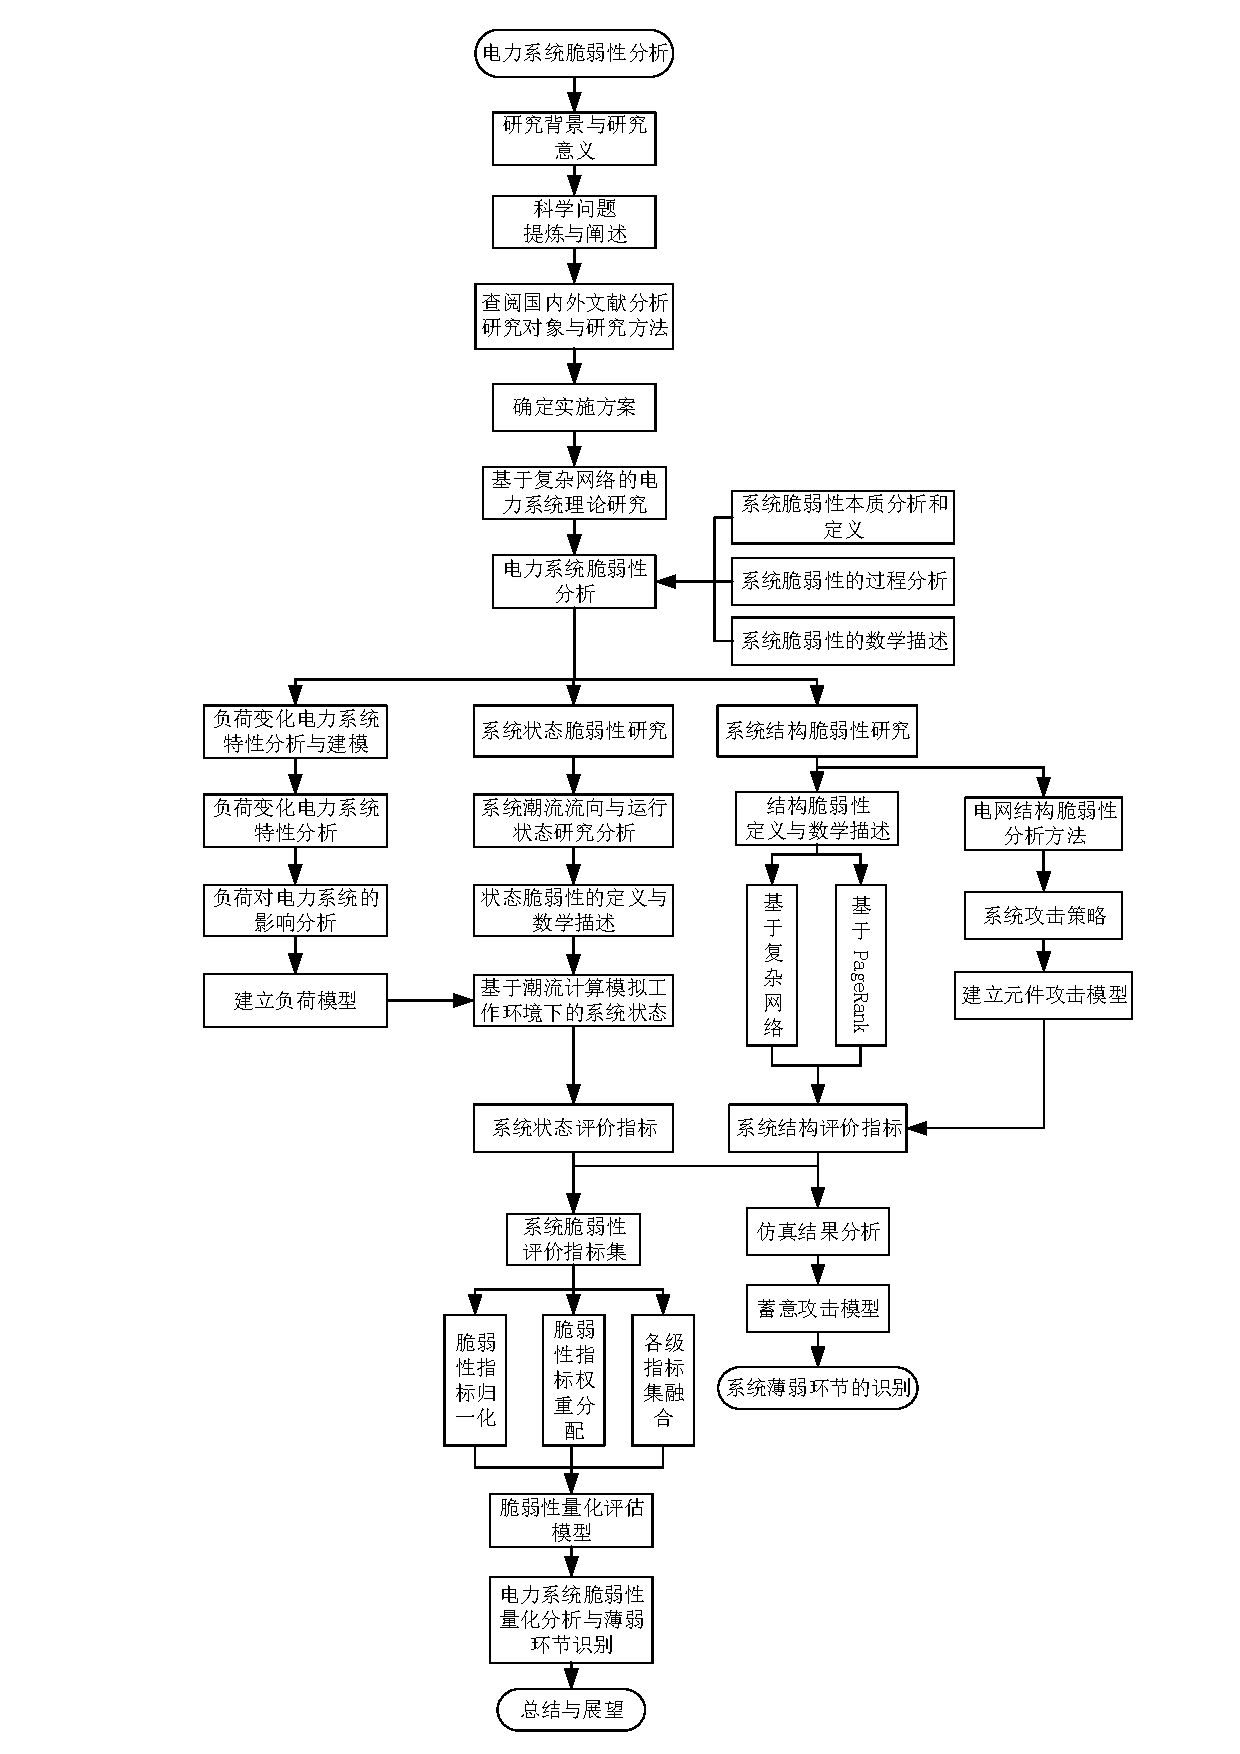
\includegraphics[height=23cm]{technicalRoute.pdf}
  \caption{技术路线图}
  \label{fig:technicalRoute}
\end{figure}

\chapter{基于复杂网络理论的电网模型验证分析}
\label{cha:model}

\section{引言}
\label{sec:index2}
经典的电力网络分析是基于基尔霍夫电流电压方程、固定的拓扑结构来进行分析的。其研究已形成了较为完善的体系\cite{refs60}。随着科学技术的不断发展,电力系统
变得越来越复杂、规模越来越大。在网络拓扑和分析计算上,经典的电力网络分析方法因节点和线路复杂度高的问题上已不再适用。而从复杂网络角度来看,电力系统可以
简化成一个由节点(母线)和边(支路)构成的网络。在复杂网络理论的基础上进行电网结构研究分析,已成为电网结构脆弱性分析的发展趋势。

电力系统作为典型的复杂网络,在研究电力系统脆弱性之初,有必要对复杂网络的相关概念进行阐述和分析。本章首先阐述复杂网络的基本概念,在此基础上分析其基本特征
参数。此外,基于复杂网络的建模方法,分析验证复杂网络的两类模型,小世界模型和无标度模型。最后,在基本特征参数的基础上,分析与描述复杂网络的脆弱性,并研究
其脆弱性常用指标,为后续章节的电力系统结构脆弱性分析实验打下基础。

\section{复杂网络基本概念}
\label{sec:powersys}
复杂网络理论是把一个复杂系统抽象为网络,将复杂系统内的各个元件视为网络的节点,将元件之间的联系抽象为复杂网络中连接各个节点的边,由此建立起复杂网络模型。
复杂网络的基本概念主要包括复杂网络的概念描述和统计描述,概念描述主要包括复杂网络语言描述和特点及特性描述。统计描述主要包括网络的基本特征参数和静
态特性,研究复杂网络的基本概念对分析后续电力系统脆弱性指标有着重要的意义。

\subsection{复杂网络概念描述}
\label{sec:composite}
复杂网络这一概念,人们试图严格去定义复杂系统,但直到现在还未充分认识和了解复杂网络,故难以给出其严格和实用的定义\cite{refs61}。目前普遍认同的是,钱学森
院士等人发起研究的系统科学研究领域——开放的复杂巨系统理论中对复杂网络的定义:具有自组织、自相似、吸引子、小世界、无标度中部分或全部性质的网络称为复杂网络
\footnote{摘自中文维基百科}。下面其性质进行具体阐述:

$(1)$自组织:对于这一概念,从不同学科角度来看会有不同的解读,我们从系统论的观点来看,“自组织”是指一个系统在内在机制的驱动下,自行从简单到复杂、从粗糙
向细致方向发展。不断提高自身的复杂度和精细度的过程。其与“他组织”的区别在于:“他组织”是靠外部指令而形成的组织,而“自组织”是系统按照内在机制自动形成的有序结构。
一个系统自组织属性愈强,其保持和产生新功能的能力也愈强。

$(2)$自相似:是指复杂网络的总体与部分、这一部分与另一部分之间的精细结构或性质所具有的相似性,或者可以这样理解:从整体中取出局部(局域)能够体现整体的基
本特征。

$(3)$吸引子:是微积分和系统科学论中的概念。一个系统有朝某个稳态发展的趋势,这个稳态叫做吸引子。吸引子是一个数学概念,描述系统运动的收敛类型,它存在于相平面。
简言之,吸引子是一个集合,当时间趋向于无穷大时,在任何一个有界集上出发的非定常流的所有轨迹都趋向于这个集合。

$(4)$小世界性:网络的小世界性是指对具有较短平均路径又具有较高聚类系数的网络性质的一种定义。平均路径长度和聚类系数会在下一小节展开描述。

$(5)$无标度性:网络的无标度性是指对网络的度分布符合幂律分布的复杂网络性质的一种定义。具体来讲,复杂网络只有少数节点拥有大量的连接,而大部分节点却很少。

% 在以上系统科学的角度理解的基础上,给出以下对复杂网络比较直观的特性论述:

%$(1)$开放性

%复杂系统是开放的,受外界影响,复杂系统及其子系统与系统的环境之间有物质、能量和信息的交换。

%$(2)$复杂性

%复杂系统中的子网络的种类繁多,子网络之间存在多种形式、多种层次的交互作用。

%$(3)$进化涌现性

%在特定条件下,系统中各元件或各子系统之间相互作用。在此期间会有微小变化,但系统能自组织、自加强、自协调,并随之扩大、发展,发生质变。这种质变,在复杂系统中称为
%涌现。


\subsection{复杂网络统计描述}
\label{sec:feature}
在刻画复杂网络结构的统计特性上提出了许多概念和特征参数,其中包含四个基本的特征参数:度及度分布、平均路径长度、聚类系数和介数及介数分布。一般一个无权无向的抽象网络用
$\boldsymbol{M}=(\boldsymbol{V}, \boldsymbol{E})$表示,$\boldsymbol{V}$为节点集合,$\boldsymbol{E}$为边集合。

$(1)$节点度及度分布:

节点$v_i$的度$k_i$定义为与该节点连接的所有节点的数量。直观来讲,一个节点的度越大,这个节点在某种情况下越重要。

网络的度分布可用分布函数$P(k)$来描述,$P(k)$的定义为网络中度为$k$的节点数量在整个网络中所占的比例,换言之,网络中节点度为$k$的概率为$P(k)$

$(2)$平均路径长度:

将网络中两个节点$v_i$和$v_j$之间的距离$d_{ij}$定义为连接这两个节点的最短路径上的边数,$L$定义为所有节点对之间最短距离的均值。

\begin{equation}
    \label{equ:chap3:feature}
    L=\frac{1}{C_N^2} \sum_{i \neq j} d_{i j}
\end{equation}

式中:$N$为网络节点数。

$(3)$聚类系数:

聚类系数是一个表征两个节点间连接紧密程度的特征参数。当节点$v_i$的节点度为$k_i$,那么相邻节点之间的边数最大为$\frac{k_i(k_i-1)}{2}$,假设节点$v_i$的$k_i$和邻居节点
之间实际存在的边数为$E_i$,那么节点$v_i$的聚类系数定义为:$C_i=\frac{2E_i}{k_i(k_i-1)}$。网络的聚类系数为:

\begin{equation} 
    \label{equ:chap3:feature}
    C=\frac{1}{N} \sum_{i=1}^N C_i
\end{equation}

式中:$N$为网络节点数。

$(4)$介数及介数分布

网络中的不相邻节点$v_i$和$v_j$之间的最短路径会途经某些节点或边,如果某些节点$v$或边$e$被其他许多最短路径经过,则表示该节点对网络的贡献较大,重要性也越高。将节点介数
$B(v)$和边介数$B(e)$分别定义为:

\begin{equation} 
    \label{equ:chap3:feature}
    B(v)=\sum_{i \neq j\in V} \frac{\sigma_{ij}(v)}{\sigma_{ij}} 
\end{equation}
\begin{equation} 
    \label{equ:chap3:feature}
    B(e)=\sum_{i \neq j\in V} \frac{\sigma_{ij}(e)}{\sigma_{ij}} 
\end{equation}

式中:$\sigma_ij$是节点$v_i$和$v_j$间最短路径的数量,$\sigma_ij(v)$是节点$v_i$和$v_j$通过节点v的最短路径数量,$\sigma_ij(e)$是节点$v_i$和$v_j$通过支路e的最短路
径数量。

\section{基于复杂网络理论的电网模型性质分析}
\label{sec:wind}

\subsection{小世界模型}
\label{sec:windEffects}
在复杂网络理论中,将现实中的复杂网络抽象成节点和边,比如人脉、互联网和电网。Watts和Strogatz将具有高聚集程度、小平均距离的这一类网络称为小世界网络\cite{refsWS}。提出小世界模型
(WS模型)。其构造过程为:首先构造一个最近邻连接的规则网络,然后以概率$p$随机断开网络上的一条边后重新连接边。当$p$为0时,网络为规则网络,当$p$为1时,网络为随机网络。当$0<p<1$
时,网络为小世界网络。当重连概率$p$介于0—1变化时,网络模型的聚类系数和平均距离也在发生变化,其演变过程如图\ref{fig:SW}所示。因小世界网络具有聚集系数高、平均距离小的特征,所以
小世界网络体现出少数随机连接的重要作用。
\begin{figure}[H] % use float package if you want it here
    \centering
    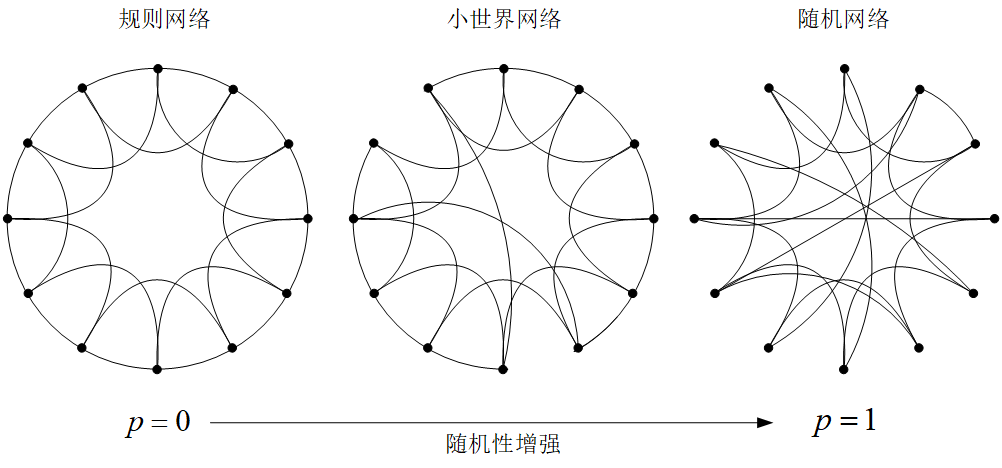
\includegraphics[width=14cm,height=6.5cm]{SW_network.png}
    \caption{小世界网络模型示意图}
    \label{fig:SW}
  \end{figure}

下面进行算例分析,取节点数$N = 1000$,初始网络规则的度$K = 6$,重连概率$p$从0-1依此增加,验证聚类系数$C$和平均距离$L$的变化过程。其验证结果如图\ref{fig:CL}所示。
\begin{figure}[H] % use float package if you want it here
    \centering
    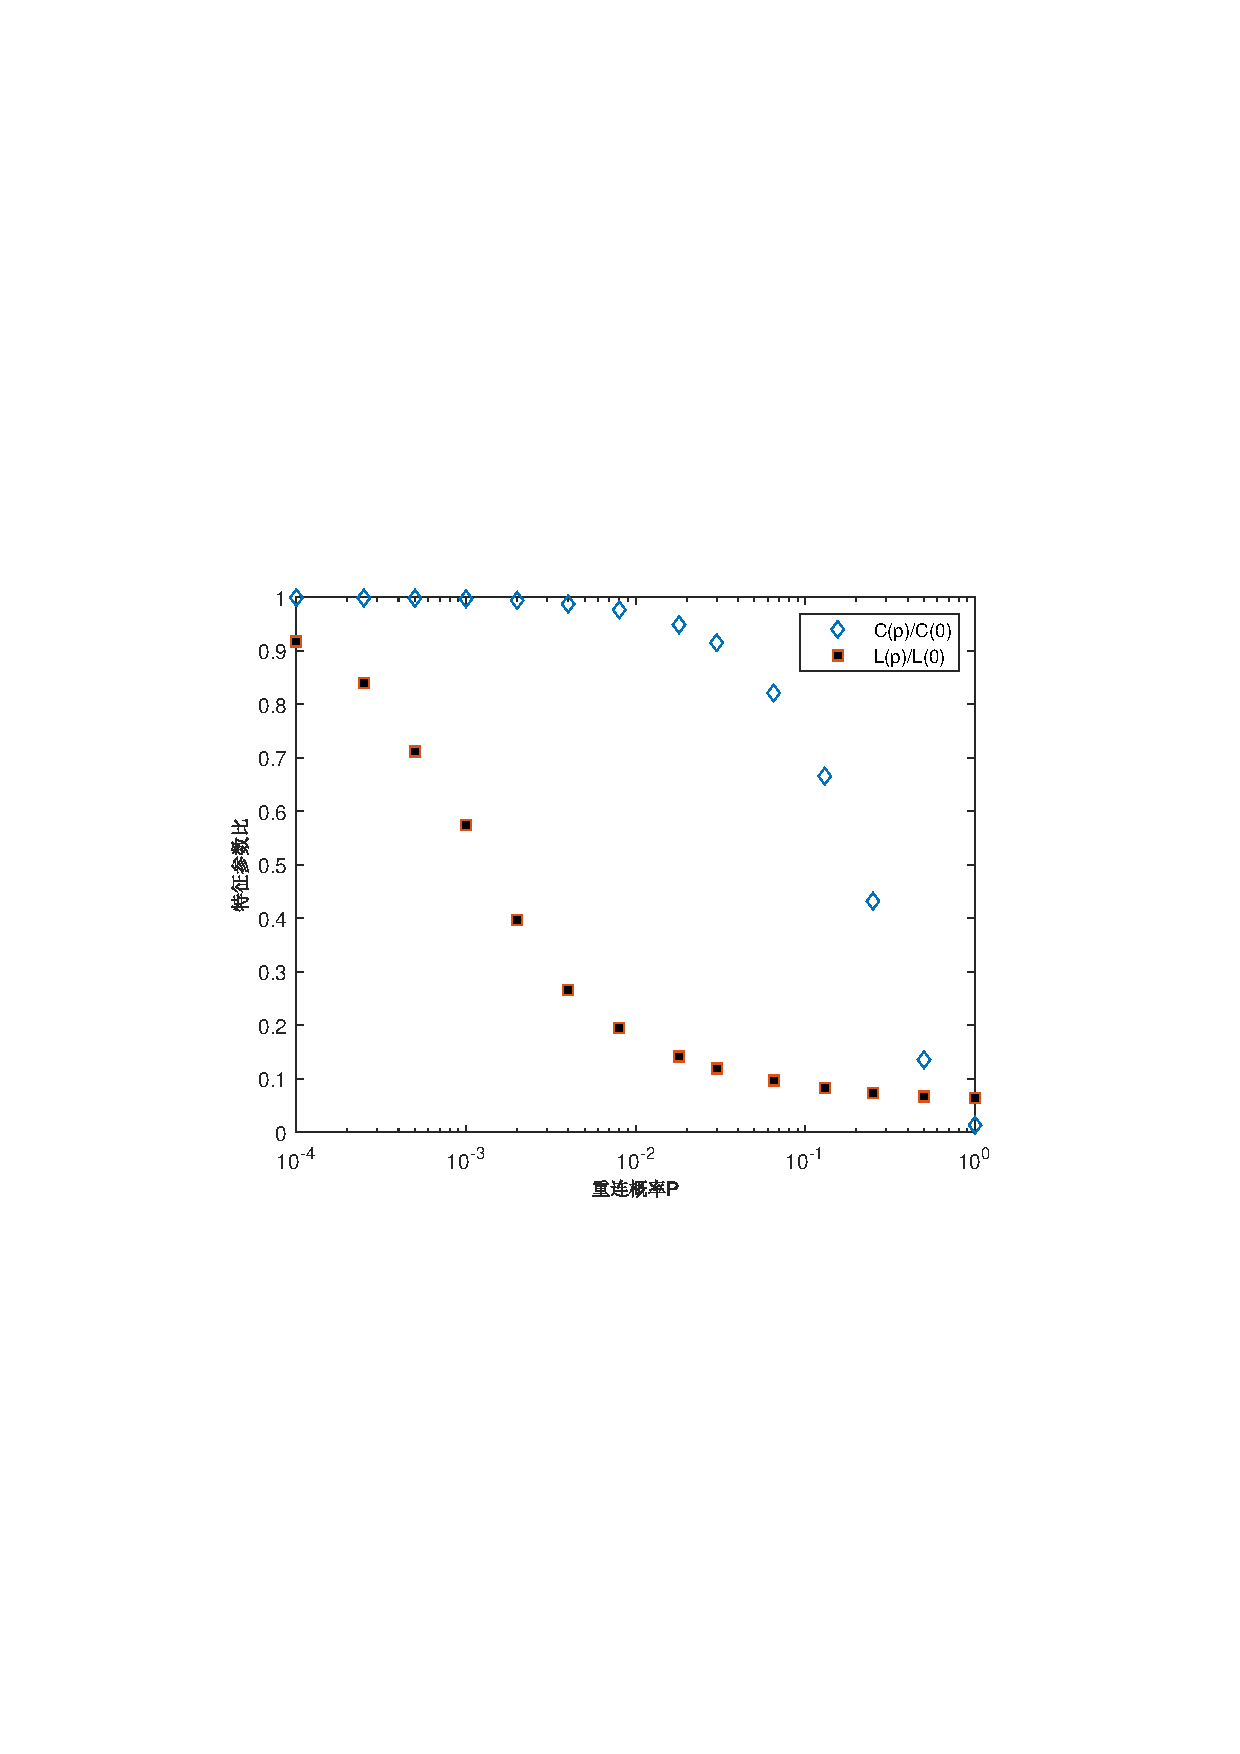
\includegraphics[]{CL.pdf}
    \caption{各重连概率$p$值下聚类系数$C$和平均路径长度$L$的变化趋势}
    \label{fig:CL}
\end{figure}

从图\ref{fig:CL}可以看出,随着重连概率$p$的增加,规则网络经历了从小世界网络到随机网络演变的过程,小世界网络相比于随机网络具有高聚集系数的特征,而相比于规则网络又具有
小平均距离的特征。其表达式如下:
\begin{equation}
\label{equ:chap2:CL}
 C\gg C_{random} \quad \quad\quad L \ll L_{regular}
\end{equation}

小世界网络模型在具体网络的应用方面具有很重要的现实意义。在网络动力学原理中,一般的网络当节点出现故障时,其影响范围很小。而在小世界网络中,由于节点间存在长程连接,节点故障
可能会快速传播到网络其他区域,进而引起网络的连锁故障。小世界网络的特征路径长度和聚类系数与故障传播的深度和广度由密切关系。一般地,特征路径路径长度越小,则故障传播就越深;
聚类系数越大,故障传播就越广\cite{refsWS1}。

为验证电力系统网络具有小世界特性,下面通过MATLAB工具分别利用$IEEE$30、$IEEE$39和$IEEE$57标准算例模型进行验证,并与相同节点数的规则网络和
随机网络进行对比分析。$IEEE$30、$IEEE$39和$IEEE$57标准算例模型的边数分别为41、46、81。规则网络采用的是最近邻耦合网络,所有的节点只与其最近的$K$个邻居节点相连,因此令规则网络
的边数约等于标准电网模型的边数,$K=2$。并在此规则网络上构建随机网络,重连概率$p$为$0$,取1000次仿真计算结果的平均值为最终值,其仿真结果如表\ref{tab:ieee}、\ref{tab:regular}、\ref{tab:random}所示。
\begin{table}[htb]
    \centering
    \caption{$IEEE$标准算例特征参数计算结果}
    \label{tab:ieee}
      \begin{tabular}{C{3cm}C{3cm}C{3cm}C{3cm}}
        \toprule
        $IEEE$标准算例      & $IEEE$30节点 & $IEEE$39节点 & $IEEE$57节点\\
        \midrule
        聚类系数($C$)       & 0.2348       & 0.0385      & 0.1222 \\
        平均路径长度($L$)   & 3.3057       & 4.7490      & 4.9536 \\
        \bottomrule
      \end{tabular}
  \end{table}

\begin{table}[htb]
    \centering
    \caption{规则网络特征参数计算结果}
    \label{tab:regular}
      \begin{tabular}{C{3cm}C{3cm}C{3cm}C{3cm}}
        \toprule
        规则网络            & 30节点        & 39节点      & 57节点\\
        \midrule
        聚类系数($C$)       & 0             & 0           & 0 \\
        平均路径长度($L$)   & 10.3333       & 13.3333      & 19.3333  \\
        \bottomrule
      \end{tabular}
\end{table}

\begin{table}[htb]
    \centering
    \caption{随机网络特征参数计算结果}
    \label{tab:random}
      \begin{tabular}{C{3cm}C{3cm}C{3cm}C{3cm}}
        \toprule
        随机网络            & 30节点        & 39节点      & 57节点\\
        \midrule
        聚类系数($C$)       & 0.0389       & 0.0275       &  0.0208 \\
        平均路径长度($L$)   & 7.6711        & 8.5568        & 9.1382  \\
        \bottomrule
      \end{tabular}
\end{table}

为了直观显示,规则网络、$IEEE$标准电网和随机网络聚类系数和平均路径长度的对比值如图\ref{fig:Cluster}、\ref{fig:L_mean}所示。
\begin{figure}[H] % use float package if you want it here
    \centering
    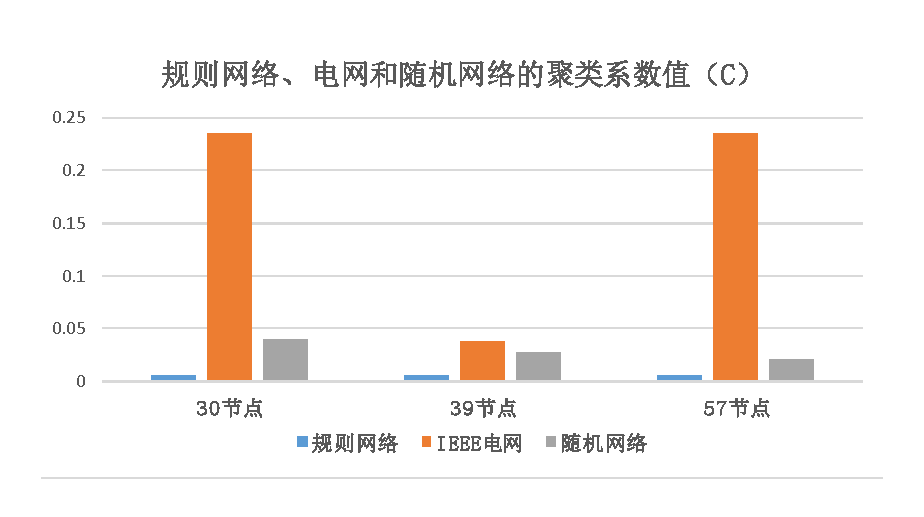
\includegraphics[width=10cm,height=5cm]{Cluster.pdf}
    \caption{规则网络、电网和随机网络的聚类系数结果图}
    \label{fig:Cluster}
\end{figure}

\begin{figure}[H] % use float package if you want it here
    \centering
    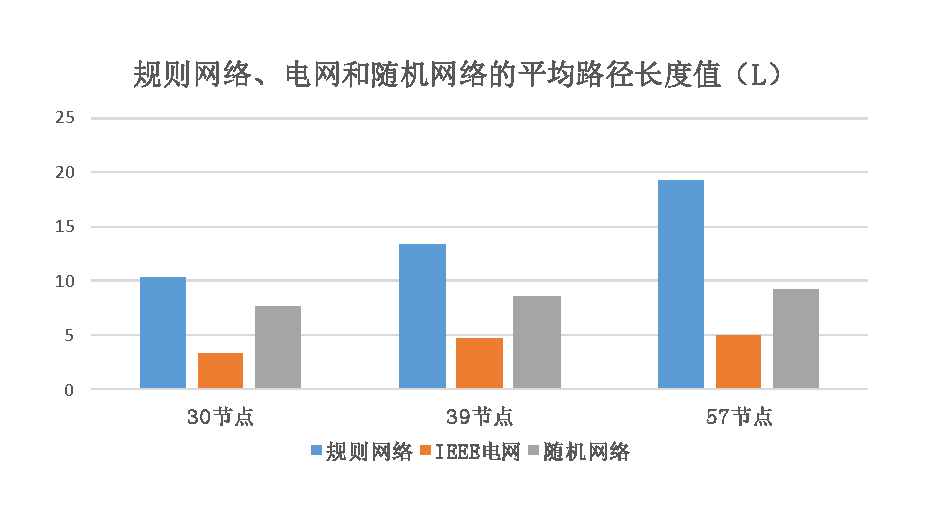
\includegraphics[width=10cm,height=5cm]{L_mean.pdf}
    \caption{规则网络、电网和随机网络的平均路径长度结果图}
    \label{fig:L_mean}
\end{figure}

从表\ref{tab:regular}可以看出,在规则网络中,节点30、39、57网络的聚类系数均为0,这是由于每个节点的度数都为 2,因此该规则网络中任意节点的邻居节点都互相不连接,故聚类系数为0。
从图\ref{fig:Cluster}和图\ref{fig:L_mean}验证了式\ref{equ:chap2:CL}的正确性,可以直观看出,实际电网系统的聚类系数远大于随机网络的聚类系数,其平均路径长度远小于规则网络的路径长度,
换句话说,电力系统网络相比于随机网络具有高聚集系数的特征,而相比于规则网络又具有小平均距离的特征,因此,验证得到电网模型为小世界网络,具有小世界性。较小的平均距离和较大的聚类系数,在
电网局部发生故障时,其故障具有较大的传播范围和传播速度。这对于研究电网的结构脆弱性具有重要的应用意义。

\subsection{无标度模型}
\label{sec:windModel}
在规则网络中,各节点的度数相同,因此规则网络的度分布集中在一个固定值上。随机网络中,由于其网络的边是以相同概率进行重连的,所以随机网络的度分布大致集中在一个概率范围内。在复杂网络理论中,
大多数现实中的网络的度数呈幂律分布,如式\ref{equ:chap2:milv}所示。因为这些网络的节点没有明显的标度,所以这种网络被称为无标度网络。
\begin{equation}
\label{equ:chap2:milv}
P(k) \propto k^{-r}
\end{equation}

在复杂网络理论中,对无标度的鲁棒性进行分析发现,随机攻击对于无标度网络结构的连通性影响很小,而攻击指定的关键环节将会对网络连通性影响很大。在电网中,电网关键节点结构的变化会对网络的连通性
造成极大的影响,进而影响电网的运行状态导致负荷损失。因此,无标度网络中的关键环节可视为电网模型的脆弱环节。下面将对电网模型的无标度性进行验证。

为了研究电网结构脆弱性,将验证电网模型的无标度特性,为此,本文选取$IEEE13659pegase$节点标准算例进行实验,通过$MATLAB$计算电网模型中各节点的度,进而得到电网的度分布结构,实验结果如图
\ref{fig:dufenbu}所示。
\begin{figure}[H] % use float package if you want it here
  \centering
  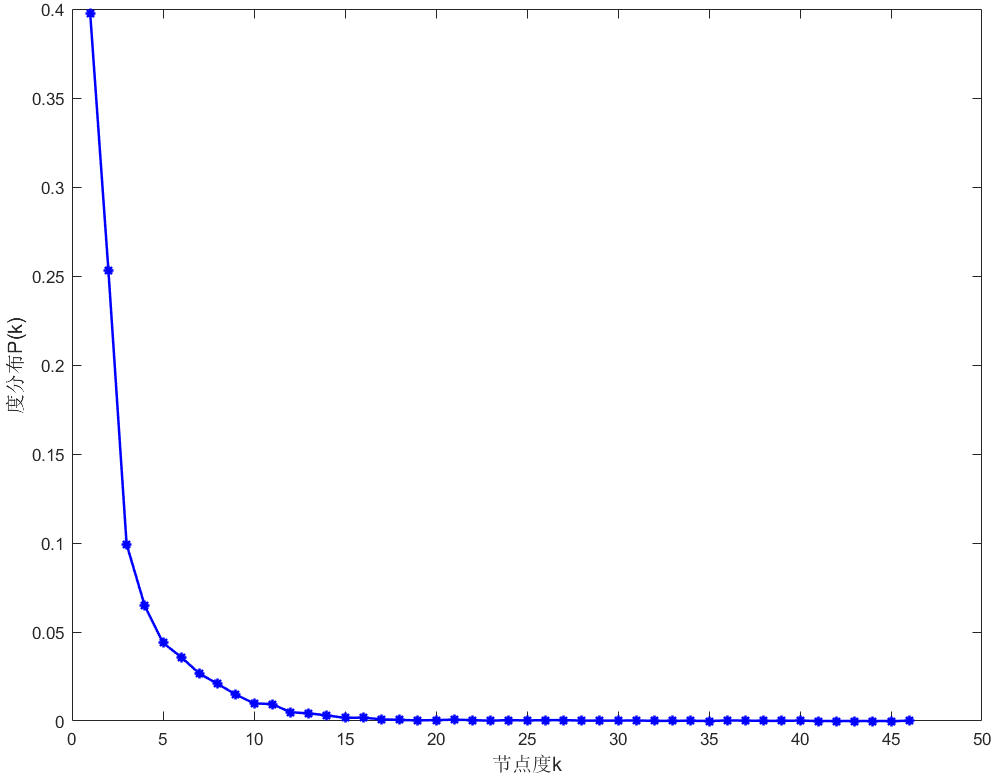
\includegraphics[width=12cm,height=8cm]{dufenbu.png}
  \caption{$IEEE13659pegase$标准算例节点度分布图}
  \label{fig:dufenbu}
\end{figure}

从图\ref{fig:dufenbu}可以看出,将近$40\%$节点度为1,节点度为2的占到了$25\%$以上,节点度为3的约占$10\%$,剩下的约占$25\%$,下面对$IEEE13659pegase$标准算例节点度分布进行幂函数拟合。
其拟合结果如图所示。
\begin{figure}[H] % use float package if you want it here
  \centering
  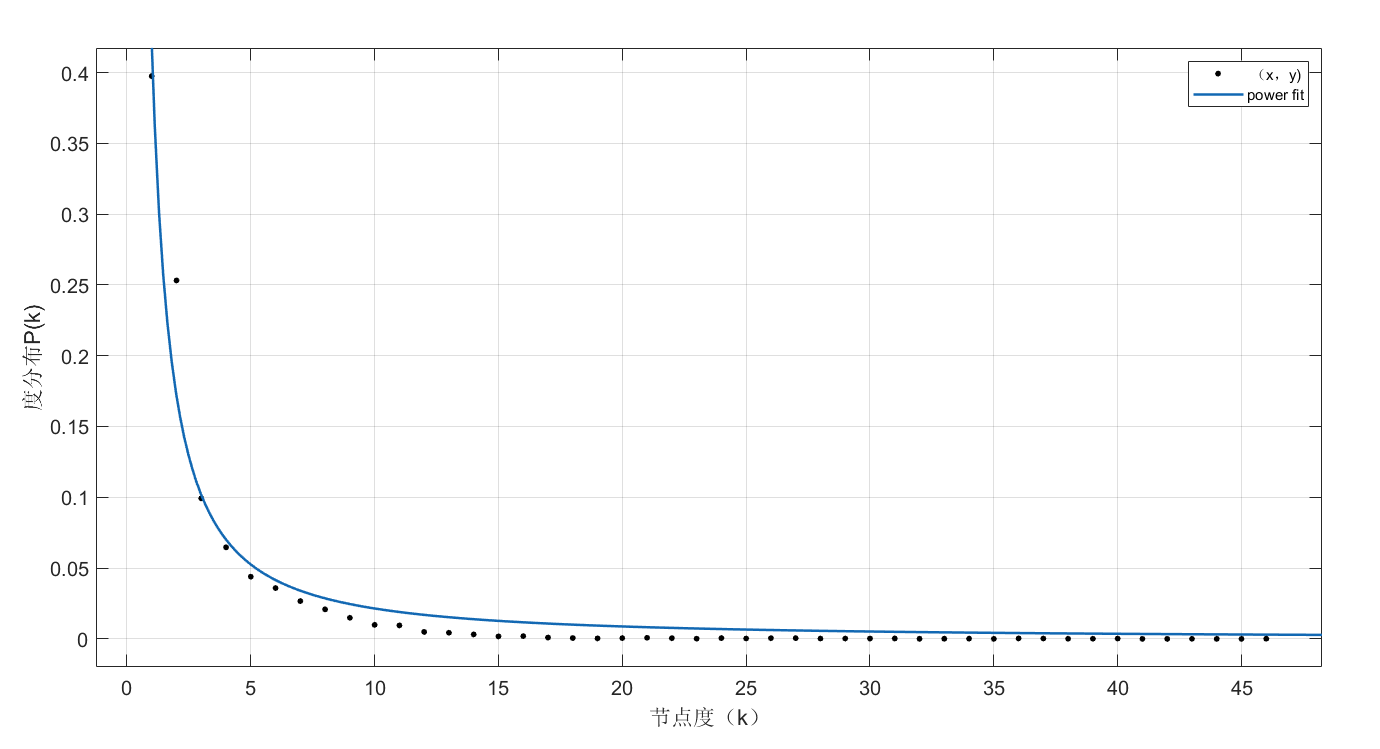
\includegraphics[width=14.7cm,height=8cm]{power_fit.png}
  \caption{$IEEE13659pegase$标准算例节点度分布拟合图}
  \label{fig:fower_fit}
\end{figure}

利用IEEE13659pegase标准算例,得到其度分布示意图,其趋势变化服从幂律分布,对数据进行数据拟合得到$p(k)=a k^{b}(a=0.4206, b=-1.292)$ 置信度为$95\%$,服从幂律分布。

在复杂网络理论中,无标度特性反映出电网具有严重的异质性,其各节点之间的连接状况(度数)具有严重的不均匀分布性:网络中少数称之为Hub点的节点拥有极其多的连接,而大多数节点只有很少量的连接。
少数Hub点对无标度网络的运行起着主导的作用。从广义上说,无标度网络的无标度性是描述大量复杂系统整体上严重不均匀分布的一种内在性质。这也表明了电网作为无标度网络的一种,当其面临蓄意的节点
攻击时较为脆弱,面临随机攻击时鲁棒的特点。通过验证电网的无标度特性,对本文提出脆弱性指标和研究电网结构脆弱性具有重要意义。

\section{复杂网络的脆弱性描述}
\label{sec:load}



\subsection{脆弱性概念}
\label{sec:loadEffect}




\subsection{脆弱性常用指标}
\label{sec:loadModel}




\section{本章小结}
\label{sec:sum2}






\chapter{电力系统结构与状态脆弱性研究分析}
\label{cha:theory}

\section{引言}
\label{sec:index3}

近年来,脆弱性一直是电力系统领域研究的热点。对于电力系统而言,脆弱性的概念目前还没有清晰明确的定义。目前大多数学者认为,电力系统脆弱性是系统本身固有的属性,
在正常运行状态下不会显现。由于电力系统内部结构的复杂性,加之对外部环境的依赖性,在外界扰动或内部结构参数作用下,电力系统的性能参数将会偏离正常范围,影响其电能
质量,因此分析电力系统的脆弱性很有研究意义。

本章将电力系统的脆弱性从两个方面进行展开分析,即结构和状态两个方面,首先从系统整体的脆弱性分析与描述入手,得到清晰合理的电力系统脆弱性本质概念和数学描述;
在此基础上,分别从结构和状态两个方面对系统脆弱性进行分析,在结构方面,主要基于复杂网络和$PageRank$理论进行分析,其脆弱性研究专注于系统受影响的程度;在状态方面,
主要基于蒙特卡洛和概率潮流方法进行分析,其脆弱性研究侧重于抗干扰能力。

\section{电力系统脆弱性分析与描述}
\label{sec:defina}

本节首先对电力系统的稳定性、可靠性以及鲁棒性进行研究分析;在此基础上,结合电力系统脆弱性的特征,得到较为明确的电力系统脆弱性本质概念;进而对电力系统的脆性过程
进行分析,并给出电力系统脆弱性的数学描述。


\subsection{电力系统稳定性、可靠性、鲁棒性的区别与联系}
\label{sec:network}

对于电力系统而言,在进行电力系统脆弱性研究分析之前,有必要明确电力系统脆弱性的概念,不可避免要涉及到系统的稳定性、可靠性以及鲁棒性。这些系统性能概念的提出是为解决
不同的工程实际问题,然而这些概念本身又有相互重叠的部分,因此需要分析电力系统稳定性、可靠性、鲁棒性的概念本质,找出它们之间的区别与联系。并进一步结合电力系统脆弱性的特征,
得到较为明确的电力系统脆弱性概念。

$(1)$稳定性

电力系统的稳定性是当电力系统受到外界扰动时发生的稳定性问题。主要表现在两个方面。当电力系统受到瞬态干扰时,电力系统会偏离原平衡状态,产生偏差,在瞬态扰动消失后,电力
系统可以恢复到原平衡状态;另一方面,当电力系统受到永久性扰动时,如电力系统的节点或线路遭到破坏时,电力系统在经历一个过渡过程后,偏离原平衡状态,达到一种新的平衡状态。
通过上述的定义,电力系统稳定性主要的关注点在于扰动消失后,系统能否恢复到原平衡状态,以及在永久性扰动情况下,系统能否达到新的平衡状态,实现系统稳定运行。

$(2)$可靠性

广义上来说,可靠性是评价元件、产品、系统在一定时间及一定条件下无故障运行的能力或可能性。电力系统的可靠性是指元件、设备或系统在预定时间内,在规定条件下执行规定功能的能力
\cite{refs62}。具体来讲,对于用户而言,电力系统的可靠性是指系统向用户长时间不间断持续提供满足质量要求的电能的能力。这种能力可以通过可靠度、失效率、平均无故障间隔等来
评价。由以上定义可知,电力系统的可靠性主要的关注点在于系统在规定时间内,在规定参数下工作的能力。

$(3)$鲁棒性

鲁棒性一词是原先统计学中的一个专业术语,20世纪70年代才开始在控制理论的研究中流行起来,用来表征控制系统对特征或参数扰动的不敏感性\cite{refs63}。所谓控制系统的鲁棒性是指系统在
自身内部模型不确定性扰动及外部摄动的影响下,系统某个性能指标保持不变的能力。在电力系统中,电力系统的鲁棒性是指系统受到外界扰动或内部自身故障后,系统中绝大部分节点或线路的状
态值保持在稳定裕度范围内变化的能力。也就是说电网中绝大部分节点仍然保持连通。电力系统鲁棒性的主要关注点在于电力系统的抗干扰能力。

通过研究分析系统的稳定性、可靠性以及鲁棒性的定义来看,这三个性能指标的区别如下表所示。

\begin{table}[H]
\centering
\caption{稳定性、可靠性、鲁棒性的区别}
\label{tab:chap3:deference}
\begin{tabular}{C{3cm}C{3cm}C{3cm}C{3cm}}
\toprule
\textbf{系统性能} & \textbf{稳定性} & \textbf{可靠性} & \textbf{鲁棒性}\\
    \midrule
    产生原因       &外部扰动           &外部扰动、内部参数变化         &外部扰动、局部故障\\
    主要关注点     &系统能否回到原平衡状态或能否达到新的平衡状态 
                                          &系统在规定时间和参数下的满足性能运行指标的能力 
                                                                        &系统的抗干扰能力\\
\bottomrule
\end{tabular}
\end{table}

电力系统在稳定性、可靠性和鲁棒性的定义可知,三者的主要关注点上略有不同,如上表所示,然而在产生原因、分析思路和内在概念上,又有着内在的联系。

稳定性是电力系统的基本保障。可靠性是在稳定性的基础上,针对具体的性能指标,可靠性强调的是在规定时间保持规定指标要求运行的能力。鲁棒性是在稳定性的基础上,研究在外界扰动或发生
局部故障后,系统性能参数保持在稳定裕度范围内的能力。

与鲁棒性概念有一点类似,不同之处在于,一是脆弱性是电力系统固有的属性,任何一个电力系统都存在脆弱性,系统正常运行的情况下,不会显现;二是其耐受程度不但包括系统抗干扰的能力,还
包括系统受影响的程度;三是电力系统的脆弱性包括结构脆弱性和状态脆弱性两个方面。电力系统可靠性概念可为研究系统状态脆弱性指标提供借鉴的思路。


\subsection{电力系统脆弱性的本质及脆弱过程分析}
\label{sec:network}

复杂系统的脆弱性是指:对于一个复杂系统$S$,存在一个子系统$S_i$,对环境有强烈的敏感性,当$S_i$受到内、外因素(包括信息、物质流等因素)的扰动或攻击产生崩溃时,会使其他部分或子系统也产生崩溃,
进而导致整个复杂系统崩溃\cite{refs61}。对于复杂系统所具有的这一特性称之为复杂系统的脆弱性。

经过上一节对电力系统性能的研究分析后,结合复杂系统脆性理论,对电力系统脆弱性的本质概念进行如下研究探讨。

电力系统作为复杂系统中的一种典型系统,其脆弱性是系统本身固有的一种属性,在正常运行和工作状态下不会显现。在电力系统中,每个子系统或元件是相互关联的,当子系统或单个元件由于外界
扰动或自身参数变化而使正常运行状态改变时,会导致系统承受不确定性因素的能力变差,这种特性即为系统的脆弱性。它表现的是系统对外界扰动或自身参数变化的耐受程度。其耐受程度由两个
方面的体现,一是系统受影响的程度;二是系统抗干扰的能力。

电力系统耐受程度可通过系统性能指标进行分析,当外部扰动或内部参数改变时,系统的性能指标在稳定裕度范围内变化,说明系统的耐受程度高,系统脆弱性差,反之,系统性能参数超出稳定裕度范围,
系统性能变差,系统脆弱性强。

按研究角度的不同,将电力系统的脆弱性分为结构脆弱性和状态脆弱性。结构脆弱性研究的是电力系统中某个元件在网络拓扑的重要程度;状态脆弱性则研究的是电力系统各状态变量偏离正常运行状态
及距离临界状态的程度。

脆弱过程分析:????

\subsection{电力系统脆弱性的数学描述}
\label{sec:describtion}

通过对电力系统脆弱性本质概念的分析研究可以得出,对于电力系统而言,系统性能变化的主要原因是外部扰动对系统元件的影响以及元件内部结构参数的变化,即脆弱源。脆弱源作用于脆弱环节,使得
系统脆弱性凸显,系统性能变差。

设系统$S$由$n$个元件$C_i$组成,且$C_i$的状态用$x_i$表示,$x_i \in X \subset R^m$。如果存在一个元件$C_b$,当其结构或状态发生变化,使得$x_b \to x_B$,有
\begin{equation}
  \lim _{g\left(x_{0}\right) \rightarrow G\left(x_{s}\right)} \delta(s) \neq \delta\left(s^{-}\right)
  \end{equation}
 
式中,$\delta\left(s^{-}\right)$为系统初始稳态的性能指标,$B$为元件$C_B$的不稳定域,$G\left(x_{B}\right)$为$C_B$不稳定域的阈值函数,$g(x_b)$是衡量$C_b$元件的性能指标,
$\delta\left(s\right)$为当前系统$S$的性能指标。

复杂系统是由元件、关系、环境组成的,元件在电力系统中对应着母线节点和线路,关系对应着节点之间的连接情况和潮流分布流向,环境对应的是一切影响电力系统结构或状态参数原因的集合。研究电
力系统的脆弱性,主要就是研究在不确定的环境中各元件之间、元件与整体之间、元件与环境之间以及整体与环境之间的内在关系,本文的主要研究方向是电力系统的节点或线路受到不确定因素影响后结
构或状态发生变化,对其他元件和整个系统产生的影响。

可以看出,系统脆弱性的数学描述和定义主要在于元件的存在性对于整个电力系统的影响,即存在能够引起整个系统性能改变的元件,量化系统中的元件对整个系统的重要程度,以及如何识别出这样的元件
是电力系统脆弱性研究的一个重要方向,通过加强对脆弱环节的重点保护和电网拓扑的优化改进,从而为预防大规模停电事故和连锁故障的发生提供了参考方向。


\section{电力系统结构脆弱性研究}
\label{sec:construction}

电力系统的结构主要是指由发电节点、负荷节点和传输线路组成的网络拓扑。拓扑结构是电能传输和系统性能的基础,它决定了电能是否能够被安全、可靠、有效地从发电节点传输到负荷节点。当电力系统
拓扑结构保持完整时,是保证电力系统稳定可靠运行的基础。但是,受外界环境的干扰,人为因素和保护设备内部故障等原因的影响,拓扑结构的完整性会受到破坏,导致电力系统无法安全可靠运行,甚至
崩溃。因此,有必要分析各个节点在网络拓扑的重要程度,进而加强对重要节点的防范和预先保护,对电力系统的稳定、高效、可靠运行有重大意义。

\subsection{电力系统结构脆弱性的定义与数学描述}
\label{sec:network}

电力系统的结构脆弱性是指电力拓扑结构中节点或线路由于外界或内部因素的影响下,导致节点或线路发生故障断开后,电网保持其连通性和维持基本稳定运行状态的能力,即保持拓扑结构完整的能力。

在电网拓扑结构方面可选取一定的评估指标,来考察某一单元或某些单元退出后系统的耐受程度——系统受影响的程度。对系统结构影响程度大的节点或线路,说明其对网络拓扑结构的完整性贡献程度高,
对于这样的节点或线路称为系统结构的脆弱点。因此,可以认为对电力系统拓扑结构影响越大的节点或线路,其脆弱性程度越高。

结构脆弱性研究的是电力系统中某个单元在网络拓扑的重要程度。在电力系统拓扑结构方面,从不同方面研究得到的结构脆弱性的指标描述不同,每个方面都有其结构重要性指标来衡量一个元件$i$在系统
中的重要程度,其数学描述如下:
\begin{equation}
  A(i)=\sum_{j\in F(i)}{k(i,j)}
  \end{equation}

$F(i)$为元件$i$有关联的元件的集合,$k(i,j)$为从不同角度考虑得到的结构脆弱性表达式,表示$i$和$j$在拓扑结构上的联结程度。

% 将$A_l(i)=\sum_{j \in F(i)}{k_l(i,j)}$定义为从某一方面考虑的结构脆弱性描述,那么从各个方面考虑的结构脆弱性数学描述定义为结构矩阵$Z$,$Z=[A_1,A_2,A_3\cdots A_n]]$于是结构脆弱性
% 矩阵的数学描述为


\subsection{基于复杂网络的结构脆弱性研究}
\label{sec:network}

复杂网络的基本思想是将一个复杂系统抽象为网络,其中系统中的单个元件被视为网络的节点,而元件之间的联系被视为网络的边,由此建立复杂网络模型。基于传统的复杂网络理论,电力系统中的母线
可以被视为节点,母线之间的传输线路被视为边,线路上的阻抗被视为权重,因此整个电力系统等效为加权无向图\cite{refs64,refs65}。

在本文2.2中,复杂网络理论描述网络的特征参数有特征路径长度、节点度和节点度分布、聚类系数、介数和介数分布等。参照复杂网络特征参数定义,并结合电力系统的特点,定义“电气度”概念如下:
\begin{equation}
  e_{i}=\sum_{j=1, j \neq i}^{N} e a_{i j} \cdot e w_{i j}
  \end{equation}

式中,$e a_{i j}$为网络中邻接节点的连接情况,为 0 代表$i$,$j$不相连,为1代表$i$,$j$相连。而$ew_{ij}$代表支路潮流上的视在功率的大小。电气度指标综合考虑节点连接数量和连接强度,
衡量的是节点在拓扑形结构中承担应力的大小,是网络中衡量节点重要性的重要参数。

介数作为复杂网络的关键参数之一,被用来描述节点或者边在信息、能量传递中的重要程度。介数的概念在电力系统被称为电气介数,它反映了网络节点、支路在整个电能输送过程中的贡献程度\cite{refs66,refs67}。

假设一个电网具有$a$个母线节点,$b$条电气连接的边,那么支路$l_{mn}$的电气介数计算公式如下:
\begin{equation}
\label{equ:chap3:cb}
  C_{B}(m, n)=\left|\sum_{i \in \mathrm{G}, j \in \mathrm{D}} w_{i j} P_{m n}(i, j)\right|
  \end{equation}

式\ref{equ:chap3:cb}中,$G$,$D$分别为发电节点、负荷节点的集合。$P_{mn} (i, j)$是单位有功功率注
向发电节点$i$和负荷节点$j$时,支路$l_{mn}$ 上产生的有功功率。$w_{ij}$是发电节点$i$和
负荷节点$j$的节点对间传输电能的权重值,大小为$min(|P_i|,|P_j|)$,分别代表了发
电节点$i$在发电节点功率总和的比率和负荷节点$j$在负荷节点功率总和的比率。

电网中节点的分类分为发电节点,负荷节点,中间节点。所有的功率都是从发电节点向负荷节点传输,因此需要对上述公式进行修正得到如下的节点电气介数计算公式。
\begin{equation}
\label{equ:chap3:cb1}
C_{B}(k)=\left\{\begin{array}{ll}{\frac{1}{2}\left(\sum_{l \in \mathbf{F}(\mathbf{k})} C_{B}(k, l)+\sum_{i \in \mathbf{D}} w_{k i}\right),} & {k \in \mathbf{G}} \\ 
{\frac{1}{2}\left(\sum_{l \in \mathbf{F}(\mathbf{k})} C_{B}(k, l)+\sum_{i \in \mathbf{G}} w_{i k}\right),} & {k \in \mathbf{D}} \\
 {\frac{1}{2}\left(\sum_{l \in \mathbf{F}(\mathbf{k})} C_{B}(k, l)\right)} & {k \notin \mathbf{G}, k \notin \mathbf{D}}\end{array}\right.
\end{equation}

式\ref{equ:chap3:cb1}中,
$F(k)$指的是与节点$k$相连的所有边的集合,$C_B (k,l)$为对应支路的电气介数。节点的电气介数与拓扑中所连支路的电气介数有直接关系。

由此所有节点的电气介数计算流程图如图\ref{fig:nodeBetweenPro}所示。 
\begin{figure}[H] 
  \centering
  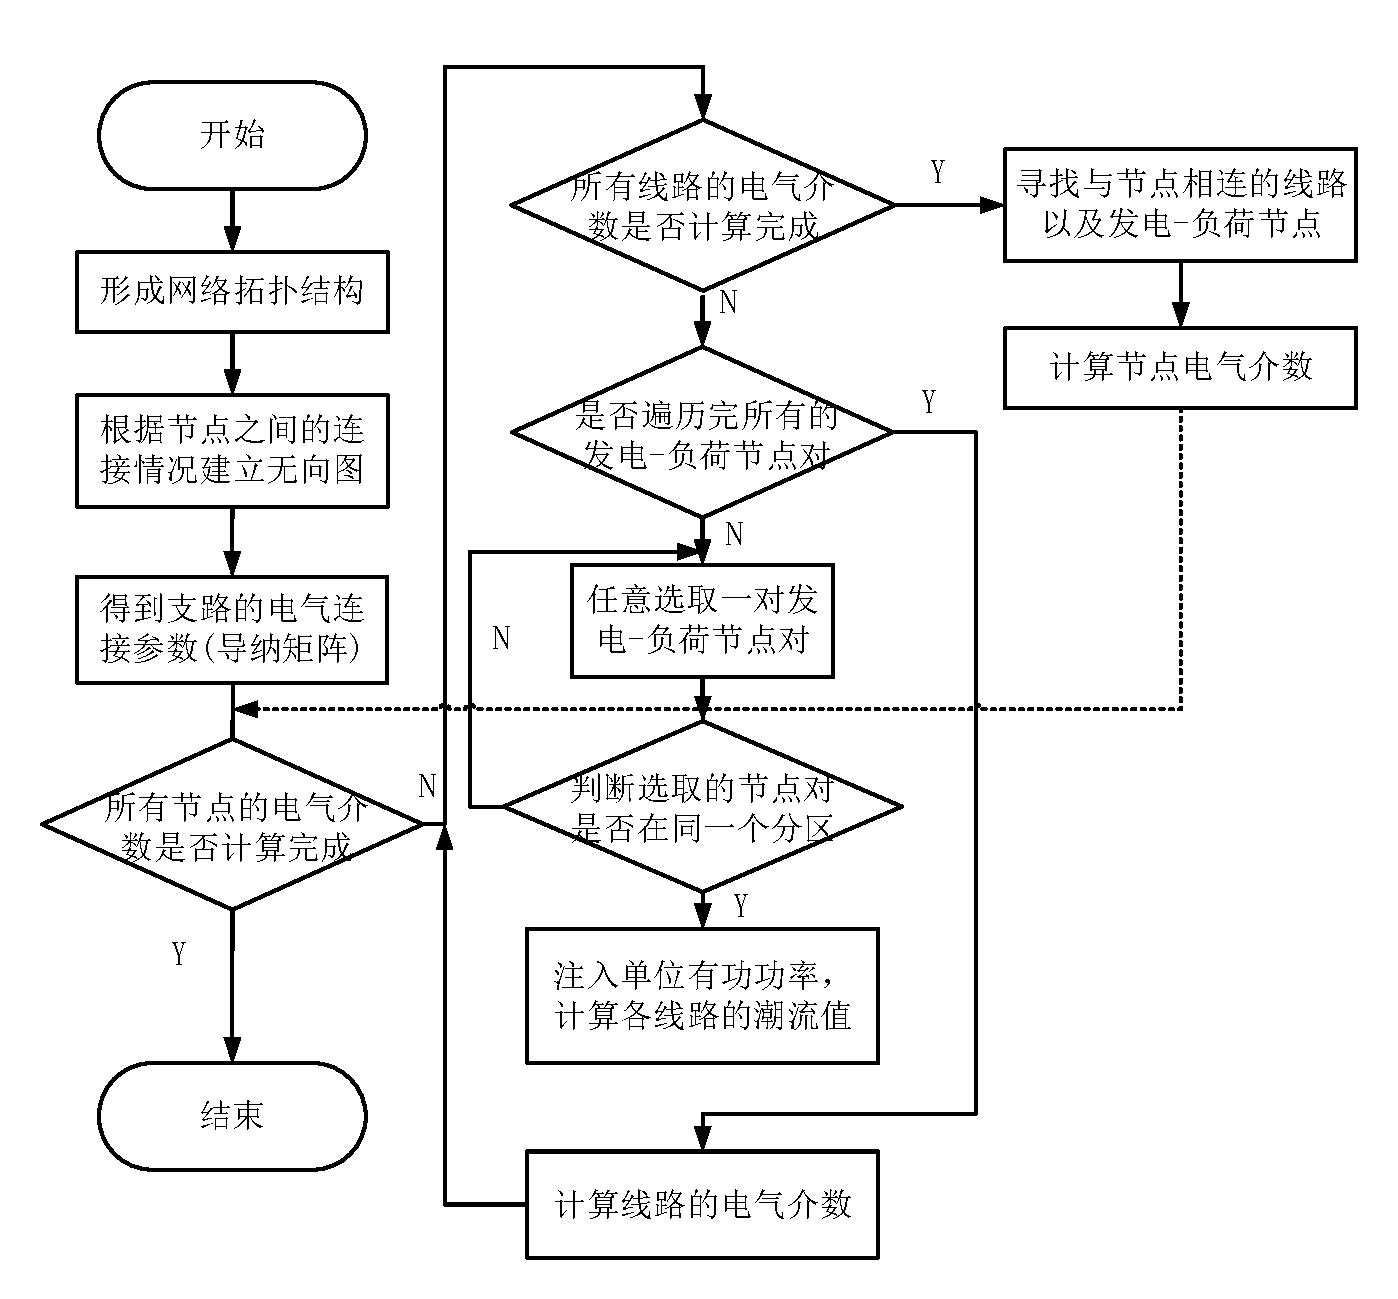
\includegraphics[height=12.7cm]{nodeBetweenProcess.pdf}
  \caption{电气介数计算流程}
  \label{fig:nodeBetweenPro}
\end{figure}

从流程图可以看出,节点的电气介数综合考虑了所连支路对其的影响。而支路的电气介数则衡量了所有发电-负荷节点对支路潮流的影响,从而在分析时,
不仅考虑了拓扑的影响而且增加了能量变化的考虑,使得结构的衡量更完善。电气介数不局限于能量、信息沿着网络的最短路径传播,更体现了电能在整个网络
支路的分布情况。同时,电气介数还分别考虑了发电节点和负荷节点的变化影响,改变他们的容量,网络各节点的重要性也会发生变化,因此,电气介数更符
合实际电网的变化情况。




$PageRank$最早是被用来作为互联网网页结构的模型,并且对所有网页进行重要度排序的一种算法\cite{refs68,refs69}。在众多计算互联网网页的相关性的算法中,$PageRank$是名气最大,
且最早被谷歌浏览器采用的。$PageRank$的基本思想是一个网页的重要性依赖于所有链接向它的其他网页。比如,网页$i$有链接指向网页$j$,如果有很多其他网页有链接指向网页$j$,那么我们认为
,网页$j$是非常重要的。另一方面,若只有一个网页有链接指向网页$j$,由于这个网页是一个权威性很高的网址,如谷歌,百度等网页,我们认为网页$j$也非常重要,因为由受欢迎、权威的网页指向它,
这份重要性将会传递下来。

在复杂系统理论中,$PageRank$算法的思想是将复杂系统等效为一个有向图。本文将电网与互联网网页搜索结合,将电力系统抽象成有向网络图,电网中,每条支路上的潮流是有确定的方向的,
所以可以被视为一个有向图。每个母线节点被视为一个网页,母线节点之间的电气连接被视为网页中的超链接,根据潮流的方向决定超链接的方向。互联网与电网的$PageRank$的拓扑模型比较
如表~\ref{tab:PRComparision}。在已有的研究中,在$PageRank$模型的网页出链的处理上采用均分的思想\cite{refs70},本文在综合考虑潮流能量对结构的影响下,认为出链是按照实际
的潮流的比重进行分配的。

按照网页的超链接可以传递重要性的思想,假设$A$节点拥有~3~个出链,它会分别按照视在功率的比例分别传递给所指向的$B$、$C$、$D$三个节点,按照潮流能量的分布作为权重。根据重要性传递规则,
可以得到能量转移矩阵$A$。对于没有出链的节点,则按照$PageRank$的算法,认为该节点对所有节点都出链,从而解决终止点的问题。因为电网的潮流能量分布中不存在自己指向自己的连接,故不存在
陷阱问题,因此不予考虑。
\begin{table}[htb]
  \centering
  \caption{互联网与电网的$PageRank$拓扑模型比较}
  \label{tab:PRComparision}
    \begin{tabular}{C{4.5cm}C{4.5cm}C{4cm}}
      \toprule
      互联网 & 电网 & $PageRank$拓扑 \\
      \midrule
      网页 & 母线 & 节点\\
      超链接 & 输电支路 & 有向边\\
      指向该网页的网页数目 & 母线进线数目 & 入度\\
      该网页指向的网页数目 & 母线出线数目 & 出度\\
      \bottomrule
    \end{tabular}
\end{table}

$PageRank$算法应用于电网拓扑的具体步骤为:

$(1)$假定初始服从均匀分布,即每个母线节点的重要性都是相同的,即对于一个一共有$n$个节点的系统而言,赋予每个网页初始相同的$PR$值,一般都为1。

$(2)$根据电网的实际潮流计算每条连接上的视在功率得到能量分布权重的矩阵P,再根据公式\ref{equ:chap3:Index3}得到能量转移矩阵A。

$(3)$迭代计算,由于每个超链接的存在都会增加对应网页的$PR$值,所以通过考虑潮流连接、能量转移情况对各个母线节点的$PR$值进行迭代更新。

$(4)$最后,经过若干次的迭代后,各个母线节点的$PR$值会趋于一个稳定的值。
\begin{equation}
\label{equ:chap3:Index3}
PR(p_i)=\frac{1-q}{N}+q\sum\limits_{p_j\in\mathbf{M_{p_i}}}{\frac{PR(p_j)}{L(p_j)}}
\end{equation}

式~(\ref{equ:chap3:Index3})中,$p_i$是被计算的节点,$M_{p_i}$是节点$p_i$的入链节点集合,$L(p_j)$是节点$p_j$的出链数目,$N$是节点总数目。$q$为阻尼系数,一般取~0.85~,引入该参数是为了解决出链为零的节点在模型计算中带来的问题,代表了当前的母线节点没有遭到破坏正常运行的概率。$1-q$则代表了节点遭到意外破坏退出运行的概率。从公式中可以看出,$p_i$节点的$PR$值与和它相连的$p_j$节点的$PR$值有关,其值越大,且$p_j$节点的出链越少,$p_i$节点的$PR$值越大。其计算流程图如下:
\begin{figure}[H] % use float package if you want it here
  \centering
  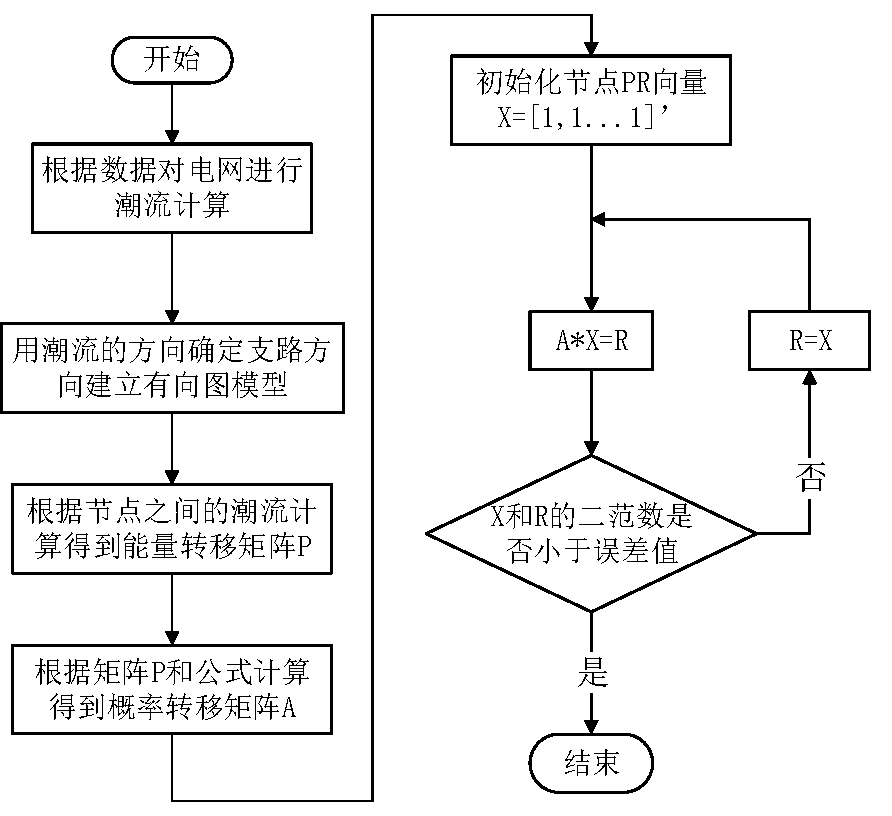
\includegraphics[height=8.4cm]{PRprocess.pdf}
  \caption{$PangRank$计算流程}
  \label{fig:PRPro}
\end{figure}

由图可知在$PageRank$在计算中,考虑更多的是节点的重要性在拓扑中的传递性。即通过反复迭代,确保所有节点的$PageRank$值在整个拓扑的重要性分配中趋于稳定,误差达到最小。$PR$值代表了节点在网络中的重要程度,$PR$值越高,节点越重要。

\subsection{模型比较与案例分析}
基于前面的研究可知,对电力系统的拓扑建模有两种不同的角度。不考虑潮流的方向,关注支路的重要性可将系统视为一个加权无向图。反之,考虑潮流的方向,衡量出入链对结构的影响可将系统视为一个有向图。复杂网络的电气介数更多关注的是支路上的潮流分布对拓扑重要性影响,而$PageRank$算法则更多关注的是有向的连接关系对拓扑重要性的影响。本节以$IEEE14$数据集为例,分别用以上的两种方式建模。该电网拓扑原理图如下:
\begin{figure}[H] % use float package if you want it here
  \centering
  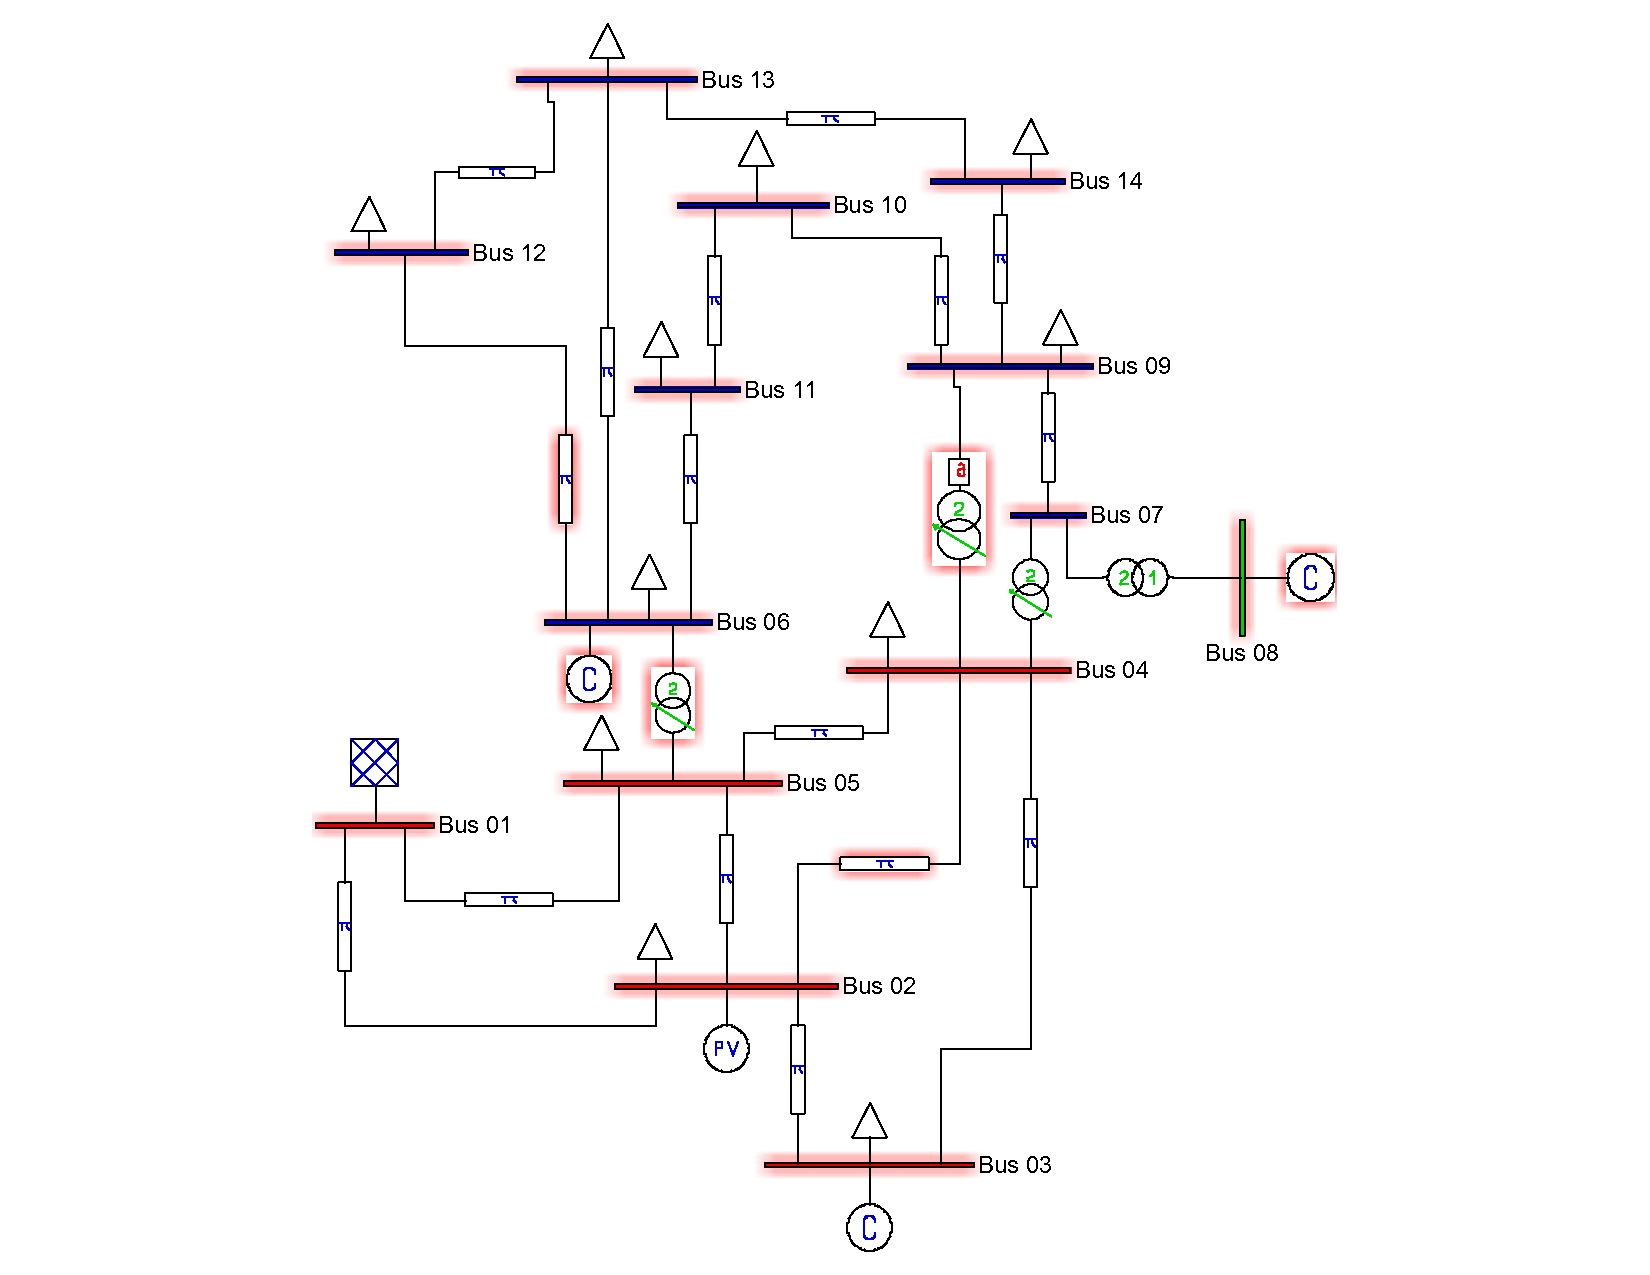
\includegraphics[height=13cm]{IEEE14.pdf}
  \caption{$IEEE14$电网拓扑原理图}
  \label{fig:fundement14}
\end{figure}

针对该拓扑,复杂网络的建模将其等效为一个无向图如图\ref{fig:model1},图中按照支路电气介数的大小等比例加粗了图的边,再根据图中的流程\ref{fig:nodeBetweenPro}最终计算得到各个节点的电气介数。电气介数计算的过程中,节点的电气介数直接受支路的电气介数影响。而支路的电气介数计算突出的是支路结构对能量分布的影响,能量分布越大的支路其电气介数也相应的越高。而$PangRank$的建模则将其等效为一个有向图如图\ref{fig:model2},再根据图\ref{fig:PRPro}最终计算得到各个节点的$PR$值。$PangRank$计算的过程中,突出的是拓扑的出入链的重要性。对于该模型,其迭代过程在能量转移矩阵的作用下完成,而入链累计度越高的点的$PangRank$越高。$PangRank$衡量了拓扑节点在能量转移中所起的作用。
\begin{figure}[H]
\begin{minipage}{0.48\textwidth}
  \centering
  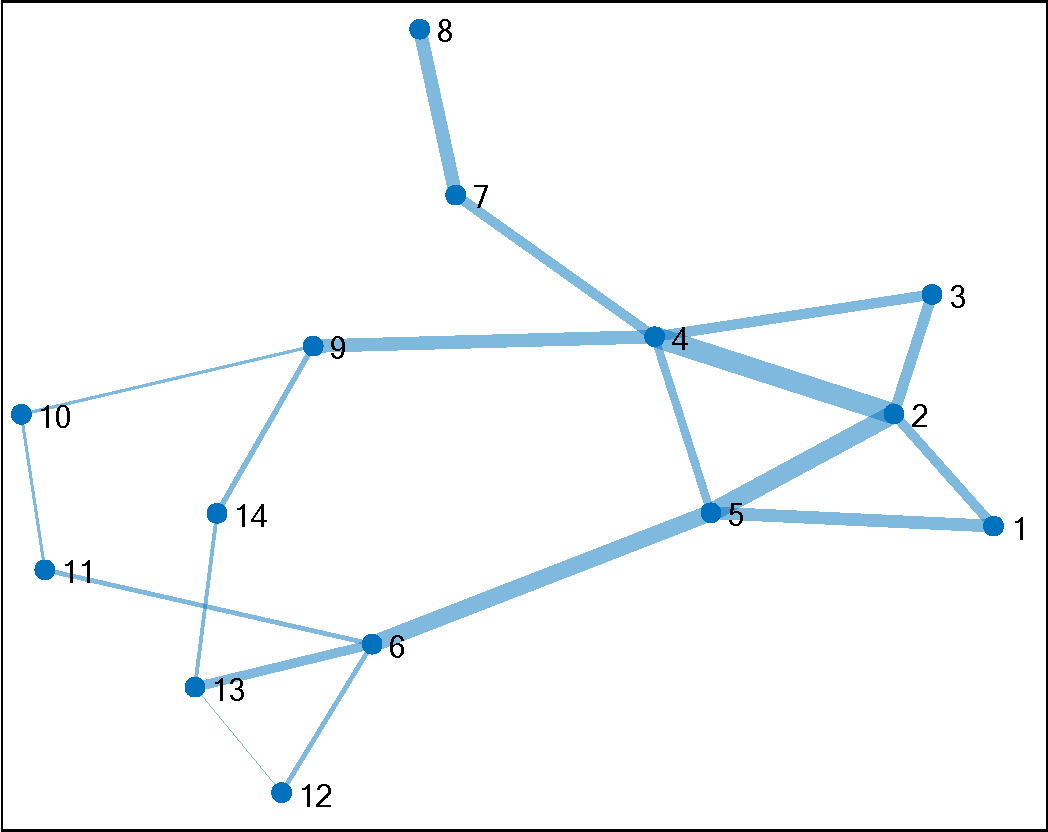
\includegraphics[height=5.8cm]{graph14.pdf}
  \caption{基于复杂网络的拓扑建模}
  \label{fig:model1}
\end{minipage}\hfill
\begin{minipage}{0.48\textwidth}
  \centering
  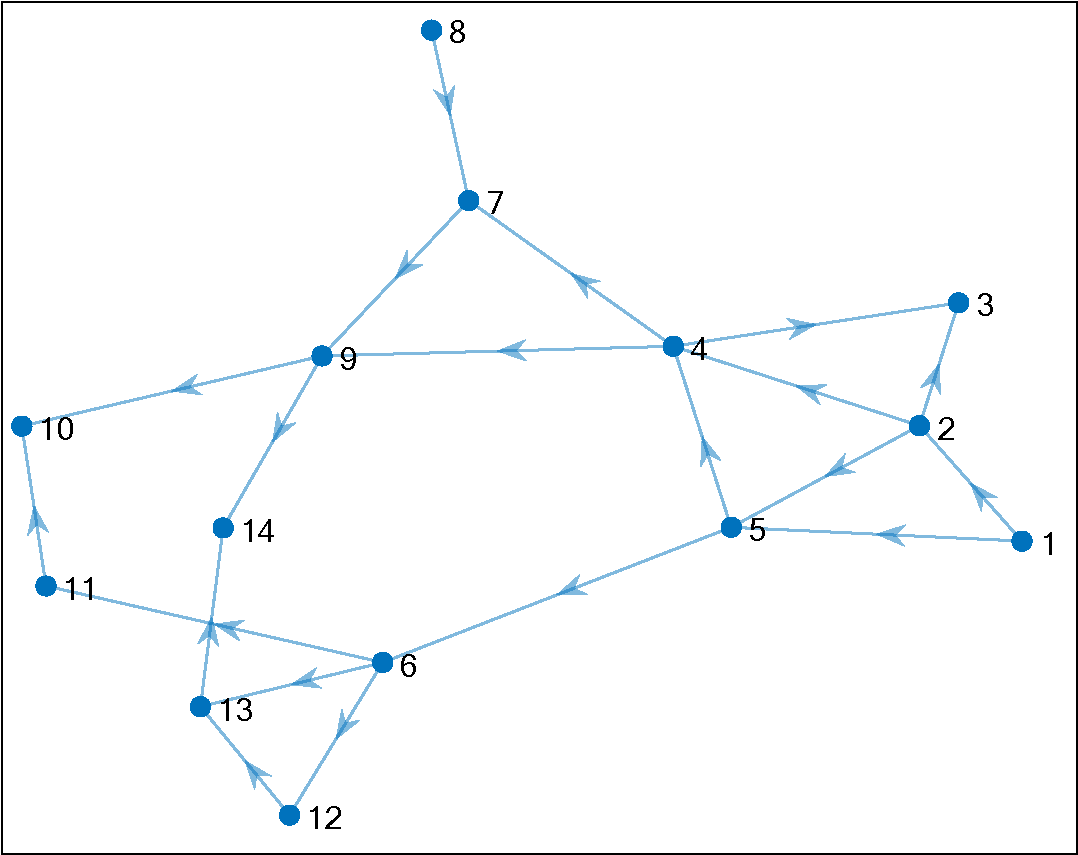
\includegraphics[height=5.8cm]{disgraph14.pdf}
  \caption{基于$PageRank$的拓扑建模}
  \label{fig:model2}
\end{minipage}
\end{figure}
电气介数与$PangRank$计算结果比较如图\ref{fig:compare_nodePR}。由于两个指标基于的拓扑模型不同,所以计算的结果相差较大。首先分析复杂网络的模型,从图中可以看出,支路的电气介数直接影响到了节点的电气介数,比如$2$、$4$、$5$节点由于与节点相连的支路比较重要而对拓扑具有较大的影响力。而支路的重要是因为$1$、$2$、$3$、$6$是系统中的发电节点,其功率传输分布因子较大,故而电电气阶数较大。而$4$、$5$处于发电和负荷的中间传输点,承担了较大的传输潮流的作用,因此相连的支路的电气介数都较大。$8$由于发电功率几乎为零且所连支路只有一条所以电气节数很小。而$12$、$11$、$10$负荷节点相连的支路都不是主要输送支路,功率传输因子小,所以电气节数较小。

反观$PangRank$的模型,该模型将每个节点的重要性赋予在该节点指向其他节点的出链上,因此,那些入链累计度高的节点重要性也高。比如$14$、$10$、$9$,这些节点均是负荷节点,能量最后传输给负荷,由于被潮流指向的累计的节点较多,即该节点的入链节点的入链节点数较多,因此重要性的权重被累计、叠加的程度较大。这种模型也符合现实,实际情况中,能量被输送、汇集到负荷节点,而负荷节点直接与用户相连,直接影响配电质量。因此,负荷节点在结构中的重要性非常高。在$PangRank$的模型中,由于发电节点是潮流起始点,$1$、$8$节点不仅是发电节点,而且是单向输出,没有其他入链,所以其$PR$值较小。

综上分析,电气介数与$PangRank$均对电力系统的结构特点进行了描述,均反映了各个节点在拓扑中的重要程度:前者从能量传输分布的角度对系统的拓扑进行了研究,后者从潮流累计分布的角度对拓扑进行了分析。因此,本文在第四章中将这两个指标进行了融合分析,作为结构脆弱性的综合评价指标。

\begin{figure}[H] % use float package if you want it here
  \centering
  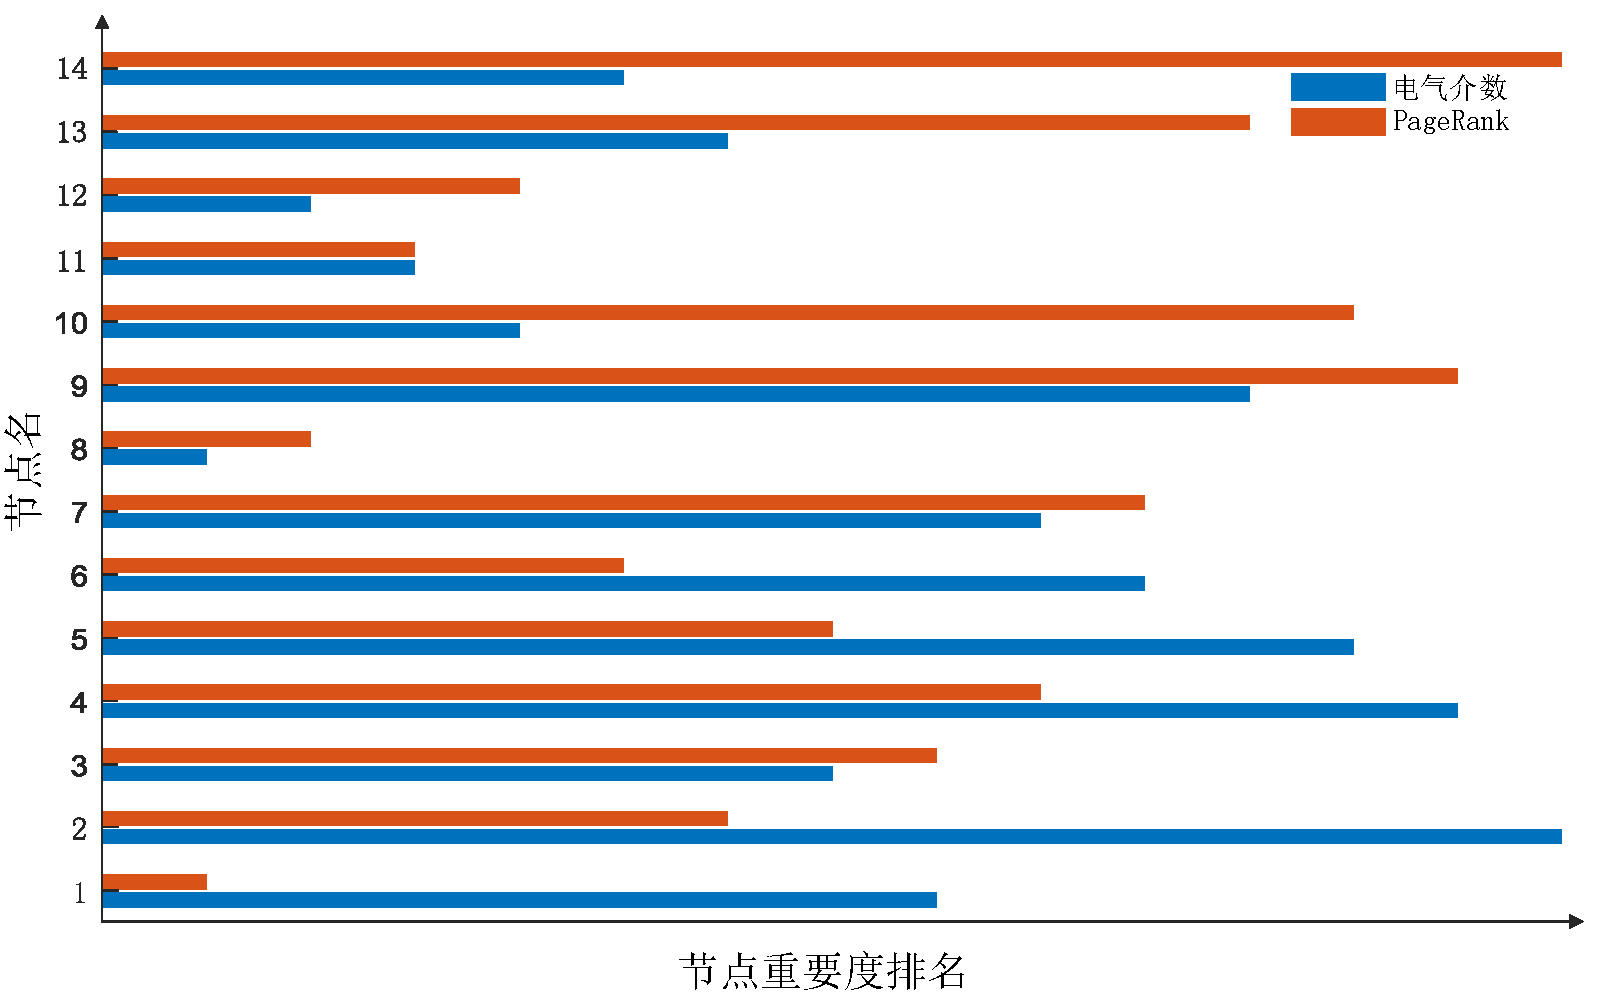
\includegraphics[height=8.7cm]{compare_nodePR.pdf}
  \caption{电气介数与$PangRank$计算结果比较图}
  \label{fig:compare_nodePR}
\end{figure}

\section{电力系统状态脆弱性研究}
\label{sec:status}

电力系统运行中,每个节点或线路都有其对应的状态变量,对电力系统而言,环境的变化会导致系统运行状态变化。环境的变化主要体现在发电节点发电容量的变化和负荷节点的负荷容量变化。
因此在电力系统状态研究中,潮流计算扮演了重要的角色。在系统的运行状态发生改变改变时,电力系统潮流分布进行重新分配。电力系统的潮流计算是计算每一种运行状态下系统的运行参数,
如电压、功率和相角等,进而判断各个运行参数是否在安全裕度范围内运行,潮流的分布是否合理是潮流计算的基本目标。


\subsection{电力系统状态脆弱性的定义与数学描述}
\label{sec:vulneStaus}

电力系统的状态脆弱性是指系统在受到外界扰动或内部自身故障后,节点或线路的状态变量发生变化,并由初始状态(额定状态)向临界点逼近的特性。表现了某个节点或线路从稳定状态向临界失稳
状态的过渡过程。反映了系统的抗干扰能力。

状态脆弱性研究的是电力系统各元件状态变量偏离正常运行状态及距离临界状态的程度。电力系统的状态量包括功率、电压、相角等。其分析方法与传统的稳定性分析方法比较接近,数学描述如下:
\begin{equation}
\Delta \alpha=\left|\alpha(t)-\alpha\left(t_{0}\right)\right|  
\end{equation}

式中:$\alpha(t)$表示节点或线路状态变量当前值,$\alpha\left(t_{0}\right)$表示节点或线路状态变量初始值(额定值),$\Delta \alpha$表示当前状态值相较于初始状态值的偏离程度。
用$\Delta \alpha_i$表示元件$i$的状态偏离程度,则电力系统各元件的状态偏离矩阵为:$D=\left[\begin{array}{lll}{\Delta \alpha_{1},} & {\Delta \alpha_{2},} & {\Delta \alpha_{3} \cdots \Delta \alpha_{n}}\end{array}\right]$

% \begin{equation}
% D=\left[\begin{array}{lll}{\Delta \alpha_{1},} & {\Delta \alpha_{2},} & {\Delta \alpha_{3} \cdots \Delta \alpha_{n}}\end{array}\right]
% \end{equation}

电力系统元件的状态偏离程度还可用百分比的形式进行表示:
\begin{equation}
  \theta=\left|\frac{\alpha(t)-\alpha\left(t_{0}\right)}{\alpha_{m}(t)-\alpha\left(t_{0}\right)}\right|
  \end{equation}

式中:$\alpha_{m}(t)$为元件状态变量的临界值,$\theta$为状态变量当前与初始稳态值的差值与临界偏差量的百分比,它表示状态的变化量相对于临界偏差的偏离程度。当$\theta<1$时,表示
元件处于正常运行状态;当$\theta>1$时,表示元件偏离临界值,元件处于失稳状态。那么电力系统各元件状态的变化量相对于临界偏差量偏离矩阵为:$E=\left[\begin{array}{lll}{\theta_{1},} & {\theta_{2},} & {\theta_{3} \cdots \theta_{n}}\end{array}\right]$

定义$f\left(\alpha_{1}, \alpha_{2}, \alpha_{3} \cdots \alpha_{n}\right)$为节点$i$或线路$i$状态变量当前值的关联函数,某一状态变量变化导致关联函数变化,当节点或线路$i$当前
状态值发生变化,其关联函数相对当前状态值变化的比值可用如下偏导式进行表达:
\begin{equation}
  \varphi=\frac{\partial f}{\partial \alpha_{i}}
  \end{equation}
将$\varphi$定义为状态灵敏度,表示当前状态值的改变对关联函数的影响程度。那么,电力系统各元件的状态灵敏度矩阵为:$F=\left[\begin{array}{lll}{\varphi_{1},} & {\varphi_{2},} & {\varphi_{3} \cdots \varphi_{n}}\end{array}\right]$

状态脆弱性的数学表达式:
  \begin{equation}
  \left\{\begin{array}{l}{\Delta \alpha=\left|\alpha(t)-\alpha\left(t_{0}\right)\right|} \\
   {\theta=\left|\frac{\alpha(t)-\alpha\left(t_{0}\right)}{\alpha_{m}(t)-\alpha\left(t_{0}\right)}\right|} \\
   {\varphi=\frac{\partial f}{\partial \alpha_{i}}}\end{array}\right.
  \end{equation}
  
系统各元件的矩阵形式的数学表达式:
\begin{equation}
  \left\{\begin{array}{l}{D=\left[\begin{array}{lll}{\Delta \alpha_{1},} & {\Delta \alpha_{2},} & {\Delta \alpha_{3} \cdots \Delta \alpha_{n}}\end{array}\right]} \\
   {E=\left[\begin{array}{lll}{\theta_{1},} & {\theta_{2},} & {\theta_{3} \cdots \theta_{n}}\end{array}\right]} \\
   {F=\left[\begin{array}{lll}{\varphi_{1},} & {\varphi_{2},} & {\varphi_{3} \cdots \varphi_{n}}\end{array}\right]}\end{array}\right.
  \end{equation}

\subsection{蒙特卡洛方法概述}
\label{sec:vulneStaus}






\subsection{负荷模型的建立}
\label{sec:vulneStaus}
结合状态三个指标的模型




\subsection{状态脆弱性分析方法及指标研究}
\label{sec:static}

在电力系统中,网络节点类型$PV$节点、$PQ$节点和$V\Theta$节点三类。

$(1)$$PV$节点:给定节点的注入有功功率$P$和节点电压有效值$U$,待求量是节点的注入无功功率$Q$ 和电压的相位$\Theta$。这类节点通常为发电机节点,其有功功率给定而且具有比较大
的无功容量,它们能依靠自动电压调节器的作用使母线电压保持为给定值。待求量为节点的注入无功功率$Q$和相位$\Theta$。

$(2)$$PQ$节点:给定节点的注入有功功率$P$和注入无功功率$Q$。这类节点对应于实际系统中的纯负荷节点(如变电所母线)、有功和无功功率都是给定的发电机节点(包括节点上带有负荷),
以及联络节点(注入有功和无功功率都等于零)。这类节点占系统中的绝大多数,待求量为节点的电压有效值$V$和相位$\Theta$。

$(3)$$V\Theta$节点:又称平衡节点,在潮流计算中,必须设置一个平衡节点,其电压有效值为给定值,电压相位为$\Theta =  0$,即系统中其他各节点的电压相位都以它为参考;
待求量为节点注入的有功功率$P$和无功功率$Q$。实际上,由于所有的 $PQ$ 节点和 $PV$ 节点的注入有功功率都已经给定,而网络中的总有功功率损耗是未知的,因此平衡节点的注入
有功功率必须平衡全系统的有功功率和有功损耗而不能加以给定,这就是平衡节点的作用。在潮流计算中,原则上可以取任一个发电机节点作为平衡节点,但通常取容量
较大出线较多的发电机节点,以便当有功功率损耗估计出入较大时,对它的注入有功功率产生的影响较小。

在电力系统潮流计算中,最根本的问题就是求解节点功率方程式,其表达式如\ref{equ:chap3:basic}所示。
\begin{equation}
\label{equ:chap3:basic}
  \left\{\begin{array}{l}{P_{i}=U_{i} \sum_{j=1}^{n} U_{j}\left(G_{i j} \cos \theta_{i j}+B_{i j} \sin \theta_{i j}\right)} \\ 
{Q_{i}=U_{i} \sum_{j=1}^{n} U_{j}\left(G_{i j} \sin \theta_{i j}-B_{i j} \cos \theta_{i j}\right)}\end{array}\right.  
\end{equation}

在电力系统潮流计算方法中,牛顿-拉夫逊(Newton-Raphson)法,简称牛顿法,是求解非线性代数方程的一种有效且收敛速度快的迭代计算方法。其求解的基本理念是已知欲求非线性方程
$f(x^{*})=0$精确解$X^{*}$的近似解$X^{(k)}$,二者之间存在误差$\Delta X^{(k)}$。将$f(X^{(k)} + \Delta X^{(k)})$使用泰勒级数展开并保留一阶导数部分
$f\left(X^{(\mathrm{k})}\right)+f^{\prime}\left(X^{(\mathrm{k})}\right) \Delta X^{(\mathrm{k})}=0$(一阶以上部分忽略不计),从中解出$\Delta X^{(k)}$。
为了达到足够高的精度要求,在估计值的基础上加上误差得到$X^{(k+1)} = X^{(k)} + \Delta X^{(k)}$,继续重复上述计算。直到迭代到解$X^{(*)}=X^{(k+1)}+\Delta X^{(k+1)}$
满足误差精度要求足够接近精确解。

上述的迭代过程可以整理成以下迭代表达式:
\begin{equation}
\left\{\begin{aligned} \Delta X^{(\mathrm{k})} &=-\left[f^{\prime}\left(X^{(\mathrm{k})}\right)\right]^{-1} f\left(X^{(\mathrm{k})}\right) \\
 & X^{(\mathrm{k}+1)}=X^{(\mathrm{k})}+\Delta X^{(\mathrm{k})} \end{aligned}\right.
\end{equation}

对于多节点的电力系统而言,$n$维非线性方程的迭代过程与一维的迭代过程大同小异,迭代表达式如下:
\begin{equation}
\label{equ:chap3:diedai}
\left\{\begin{array}{c}{\Delta X^{(\mathrm{k})}=-\left[J\left(X^{(\mathrm{k})}\right)\right]^{-1} f\left(X^{(\mathrm{k})}\right)} \\ 
{X^{(\mathrm{k}+1)}=X^{(\mathrm{k})}+\Delta X^{(\mathrm{k})}}\end{array}\right.
\end{equation}

式\ref{equ:chap3:diedai}中,$X$、$\Delta X$、$J$都是矩阵形式,运算时进行的是矩阵运算,其中$J$是潮流计算的雅可比矩阵。

潮流计算的目标是计算每种运行状态下系统的参数变化,功率或电压的分布,用来检查系统的元件是否过负荷、各点电压是否越线、功率的分布是否合理。为了保证系统能够正常运行,
潮流方程有以下约束条件:

$(1)$节点电压上下限:节点电压应小于节点最大额定电压并大于最小额定电压,即:
\begin{equation}
  V_{i \min } \leq V_{i} \leq V_{i \max } \quad(i=1,2, \cdots n)
  \end{equation}
$(2)$节点功率上下限:发电机节点功率应小于节点最大额定功率并大于最小额定功率,即:
\begin{equation}
\left\{\begin{array}{l}{P_{G i \min } \leq P_{G i} \leq P_{G i \max }} \\ {Q_{G i \min } \leq Q_{G i} \leq Q_{G i \max }}\end{array} \quad\left(i=1,2, \cdots G_{n}\right)\right.
\end{equation}

通过以上潮流计算分析,给出潮流计算流程图,如图\ref{fig:powerFlow}所示。
\begin{figure}[H] % use float package if you want it here
  \centering
  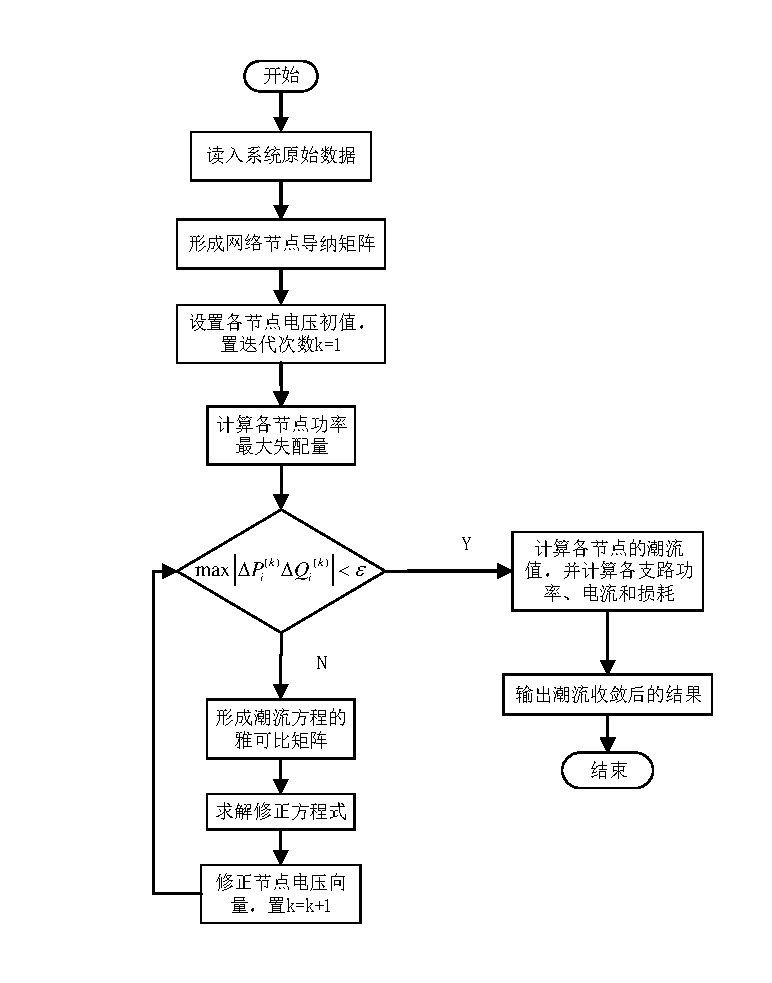
\includegraphics[]{powerFlow.pdf}
  \caption{稳态潮流计算流程图}
  \label{fig:powerFlow}
\end{figure}


在电力系统中,稳定裕度是指系统中各元件的运行状态值与临界状态值的相对距离,表征的是电力系统当前运行状态距离失稳状态的程度。

在电力系统状态脆弱性研究分析中,电力系统的节点电压是研究系统脆弱性的重要指标,电力系统各节点电压的高低实际反映的是电力系统是否正常供电。在电力系统运行过程中,保证
电压的稳定可以有效提高电力系统的运行效率,降低系统出现级联停电的可能性;除此之外,在电力系统状态研究中,负荷节点容量也是一项重要的研究指标,从大规模的停电事故中
可以看出,很多事故原因在于电力系统局部负荷过载,保证电力系统负荷节点的负荷功率在安全容量范围内,可以有效降低因局部负荷过载和级联效应而导致电力系统瘫痪事故发生的
可能性。因此,本文提出电压裕度指标和功率稳定裕度指标作为评估电力系统各元件脆弱性的指标。

在电力系统运行过程中,通过比较节点实际的运行电压和临界电压之间的裕度来评估电网各节点的状态脆弱性。定义“电压裕度”指标如下:
\begin{equation}
  S_V=\frac{U_{C}-U_{I}}{\left|\alpha U_{m}\right|}
  \end{equation}

式中,$U_C$为电压临界值,$U_I$为当前运行电压值,$\left|\alpha U_{m}\right|$为电压稳定阈值,$\alpha$为电压最大允许的波动率(偏差率)。$U_m$为负荷节点额定电压值。
电压裕度越小,说明系统元件在运行过程中极易达到失稳状态,其脆弱性越强。


在功率稳定裕度指标研究方面,本文的主要专注点在于节点所能承受最大负荷的能力,因此,通过连续潮流(CPF)计算得到各节点的最大负荷功率,并定义“功率稳定裕度”指标如下:
\begin{equation}
  S_C=\left|C_M-C_i\right|
  \end{equation}

式中,$C_M$为节点最大负荷功率,$C_i$为节点的额定功率。


灵敏度的物理意义为:控制量每变动一个单位引起的输出量的变化值。

在电力系统中,灵敏度一般是指以输出或状态向量表征的系统运行状况对控制向量和扰动向量变化的敏感程度。灵敏度分析大部分是建立在潮流方程基础上的,不同学术文献中所用到方法
的不同之处,除了在所提出的评价指标的差别外,还体现在潮流计算中对所用变量的分类和其相互关系的处理上。
基于潮流计算的灵敏度分析的基本方程是节点功率平衡方程,其极坐标形式如下:
\begin{equation}
  \left\{\begin{array}{l}{P_{i}=U_{i} \sum_{j=1}^{n} U_{j}\left(G_{i j} \cos \theta_{i j}+B_{i j} \sin \theta_{i j}\right)} \\ 
{Q_{i}=U_{i} \sum_{j=1}^{n} U_{j}\left(G_{i j} \sin \theta_{i j}-B_{i j} \cos \theta_{i j}\right)}\end{array}\right.  
\end{equation}

在灵敏度分析中,按照各变量的数学作用,可将变量分为如下四类:

$(1)$独立参数向量$\alpha$:包括线路导纳参数$G$,$B$等常量;

$(2)$状态参数向量:$S=\left[U_{l}, \theta_{l}, Q_{g}, \theta_{g}, P_{0}, Q_{0}\right]^{T}$,(潮流计算待求量)包括负荷节点的电压、相位;发电节点的无功功率、相位,
平衡节点的有功功率、无功功率;

$(3)$控制参数向量:$C=\left[P_{l}, Q_{l}, P_{g}, V_{g}, \theta_{0}, U_{0}, B, G \cdots\right]^{T}$(电网模型数据给定(输入)量)包括负荷节点的有功功率和无功功率,
发电节点的有功功率和电压幅值,平衡节点的相角和电压幅值,以及电网支路的导纳和电纳参数等;

$(4)$输出参数向量:$Y=\left[Q_{g}, P_{0}, Q_{0}, P_{L O S S}, Q_{L O S S} \cdots\right]^{T}$,(潮流计算输出量计算结果)包括平衡节点的有功功率和无功功率,以及电网
的有功损耗和无功损耗等。

下标$l$,$g$和$0$表示所对应的量为$PQ$节点,$PV$节点和平衡节点。

在电网指标的研究中,状态参数向量也可以归为输出参数向量中,作为状态脆弱性指标研究的重要参考。

按照以上变量的划分,灵敏度分析的数学方程可以表示为:
\begin{equation}
\left\{\begin{array}{l}{F(S, C, \alpha)=0} \\ {Y=G(S, C, \alpha)}\end{array}\right.
\end{equation}

在上式中,定义$F(S, C, \alpha)=0$为状态方程,包括电力系统中各节点的功率平衡方程,与式3.9等价;定义$Y=G(S, C, \alpha)$为输出方程,包含$PV$节点的无功功率方程、网损方程、
平衡节点方程、支路潮流方程等输出方程。

由于电力系统网络的复杂性,以及潮流状态方程为非线性方程,因而只能用迭代方法求其数值解,所以本文在灵敏度研究分析上,采用简便灵敏度分析方法,简化灵敏度分析过程,忽略潮流方程
变量之间的相互关系,借助牛顿潮流计算方法对其进行迭代求解。在状态方程和输出方程中对控制向量$U$求全微分:
\begin{equation}
  \frac{\partial F}{\partial S} \cdot \frac{d S}{d C}+\frac{\partial F}{\partial C}=0
  \end{equation}
\begin{equation}
  \frac{d Y}{d C}=\frac{\partial G}{\partial S} \cdot \frac{d S}{d C}+\frac{\partial G}{\partial C}
  \end{equation}

从式$3.11$中,可得到状态参数的灵敏度表达式:
\begin{equation}
  \frac{d S}{d C}=-\left(\frac{\partial F}{\partial S}\right)^{-1} \frac{\partial F}{\partial C}
  \end{equation}
  
将式$3.13$代入式$3.12$可得到输出参数的灵敏度表达式:
\begin{equation}
  \frac{d Y}{d C}=-\frac{\partial G}{\partial S}\left(\frac{\partial F}{\partial S}\right)^{-1} \frac{\partial F}{\partial C}+\frac{\partial G}{\partial C}
  \end{equation}

从以上的状态方程和输出方程可以看出,灵敏度指标从不同的变量来考虑可以构造出不同的灵敏度指标。

在电力系统状态指标的研究中,电网损耗指标是电力生产中的重要技术经济指标,它直接反映的是电网整体的能效水平。理论上讲,电网线损率高意味着电力建设落后、网架结构薄弱、
设备老化严重。因此,本文研究负荷节点的功率变化对系统支路功率损耗的影响程度,不仅可以为降低电网损耗率提供参考意见,还能识别出导致电力系统损耗率较高的关键元件。

根据式3.16,对电网损耗灵敏度表达式进行如下定义:
\begin{equation}
  \frac{d P_{LOSS}}{d P_i}=-\frac{\partial G}{\partial S}\left(\frac{\partial F}{\partial S}\right)^{-1} \frac{\partial F}{\partial P_i}+\frac{\partial G}{\partial P_i}
  \end{equation}

式中,$P_LOSS$为系统支路损耗,$P_l$为负荷节点功率。

本文就电网有功损耗对灵敏度表达式进行推导,电网有功损耗的表达式:
\begin{equation}
  P_{L O S S}=\sum_{i=1}^{n} \sum_{j=1}^{n} U_{i j}^{2} G_{i j}
  \end{equation}

式中$U_ij$为节点$i$和节点$j$的电压差,$G_ij$为节点$i$和节点$j$电导矩阵。

令$$I_j = \sum_{j=1}^{n} U_{j}\left(G_{i j} \cos \theta_{i j}+B_{i j} \sin \theta_{i j}\right)$$
$$I_i = \sum_{i=1}^{n} U_{i}\left(G_{i j} \cos \theta_{i j}-B_{i j} \sin \theta_{i j}\right)$$

根据式3.11节点功率方程式可得:
\begin{equation}
  \frac{d P_{\text {Loss}}}{d P_{i}}=2 G_{i j} \sum_{i=1}^{n} \sum_{j=1}^{n}\left[\left(\frac{P_{i}}{I_{J}^{2}}-\frac{P_{j}}{I_{I} \cdot I_{J}}\right)\right]
  \end{equation}

从上式可以看出,电网有功损耗对负荷节点的灵敏度不仅和节点注入的有功功率有直接关系,还与电网其他的控制向量参数和状态向量参数有关。所以灵敏度指标是在潮流计算的基础上得出的。

本文所采用的潮流计算方法为牛顿潮流法,这是一种求解非线性代数方程的一种有效且收敛速度快的迭代计算方法。根据节点功率平衡方程式,通过泰勒级数展开保留一阶导数部分,不断进行迭代,
缩小精确解和近似解之间的误差,直到满足精度要求为止。



基于前面的状态脆弱性指标的研究,本节已$IEEE39$电力系统数据集为例,通过连续潮流计算分别计算电力系统节点的最大负荷功率和节点功率变化对电网支路损耗的灵敏度,如图\ref{fig:PV_curve,fig:senseTest}
所示。
\begin{figure}[H] 
  \centering
  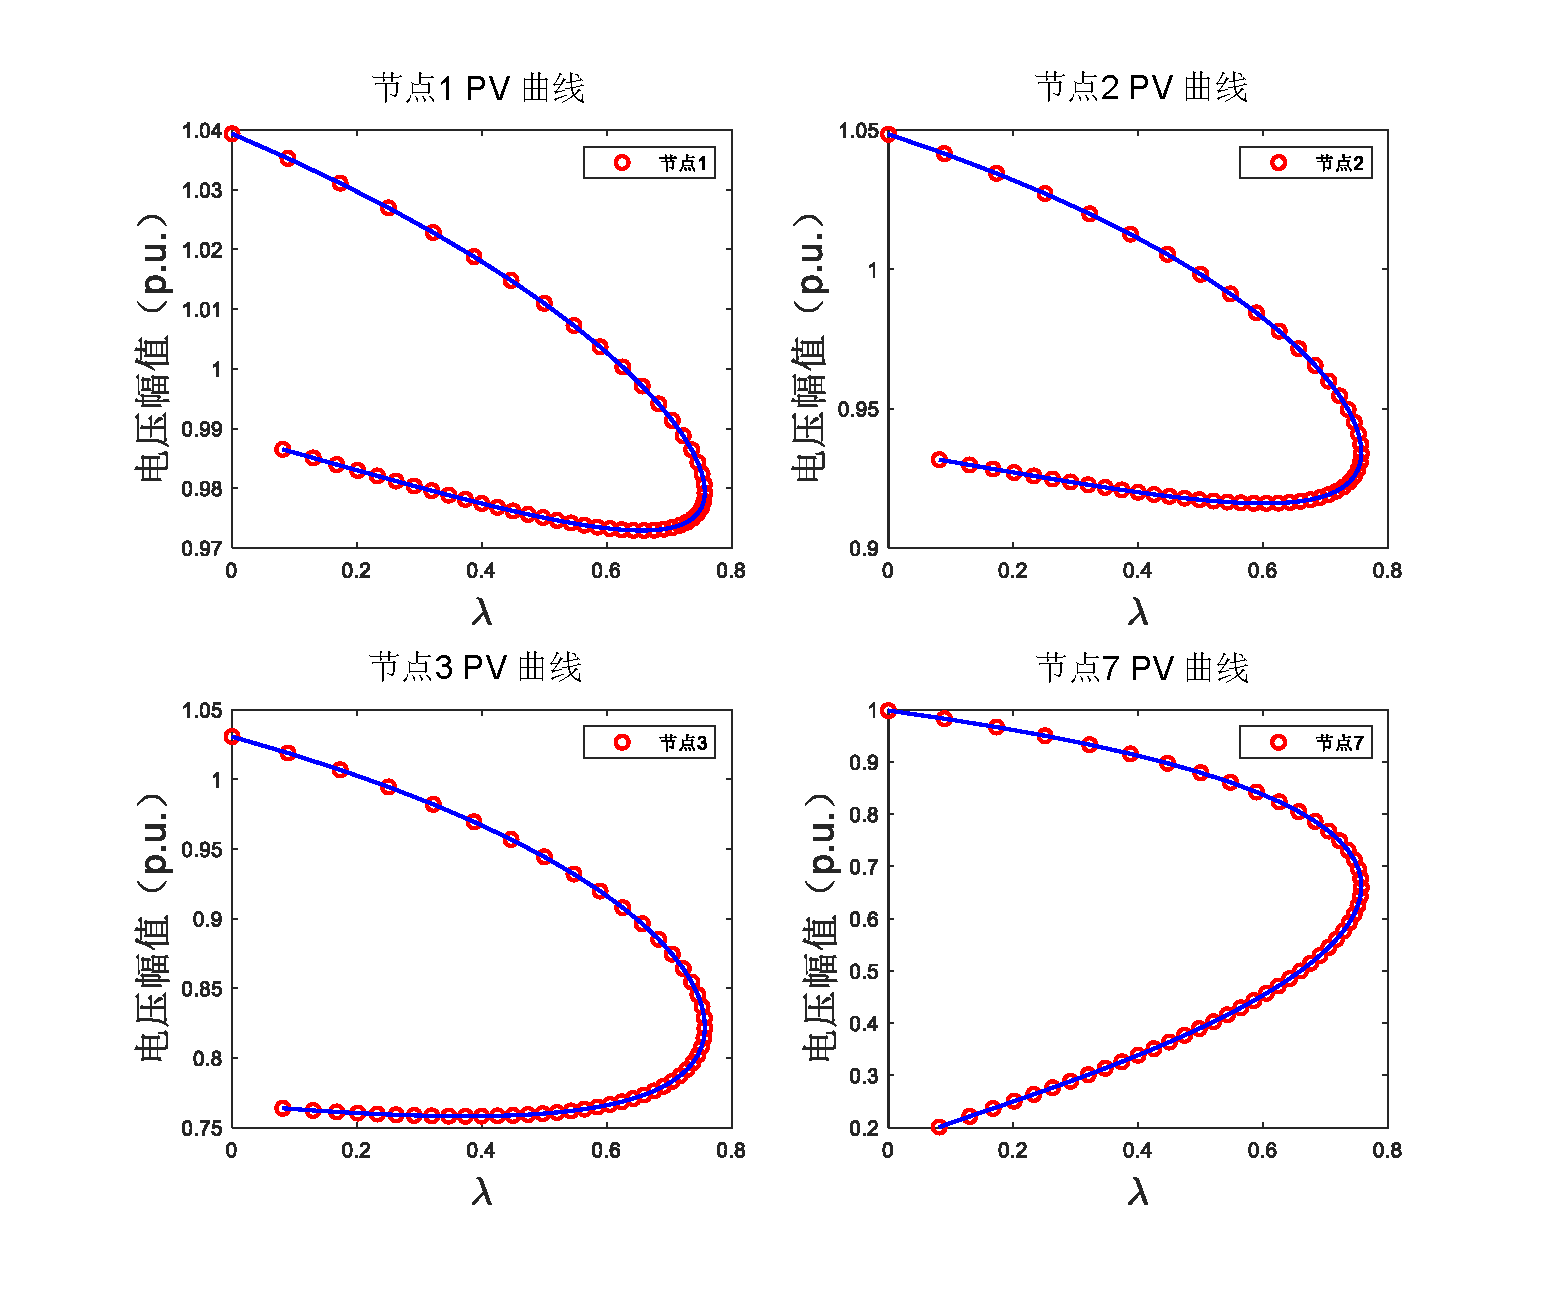
\includegraphics[height=9cm]{PV_curve.pdf}
  \caption{$IEEE39$连续潮流下PV特性曲线}
  \label{fig:PV_curve}
\end{figure}

如图\ref{fig:PV_curve}所示,$\lambda$为负荷增长率,随节点负荷的缓慢增加,不断求解潮流方程,从而描绘出系统的PV曲线。也就是说,鞍岔分节点为电力系统节点电压和功率的临界点。
可以看出,在连续潮流(CPF)计算结果中,系统中不同节点其临界电压和最大节点负荷功率不同,从而在侧面体现出电力系统的异质性。为了方便度量,在负荷增加的方式上采用的是增加负荷增长率的方式,
虽然不同节点的最大负荷增长率相同,但是其最大节点功率负荷不同。具体的临界数据如图\ref{tab:chap3:Critical}所示。
\begin{table}[H]
  \centering
  \caption{节点1、2、3、7临界电压值和最大节点有功功率值}
  \label{tab:chap3:Critical}
  \begin{tabular}{C{4cm}C{2cm}C{2cm}C{2cm}C{2cm}}
  \toprule
  \textbf{节点名} & \textbf{节点1} & \textbf{节点2} & \textbf{节点3} & \textbf{节点7}\\
      \midrule
      节点电压临界值(p.u.)   & 0.979     &0.937       &0.829      &0.660\\
      最大节点有功功率(MW)     & 208.44     &0    &687.68      &499.3\\
  \bottomrule
  \end{tabular}
  \end{table}

在表\ref{tab:chap3:Critical}中,由于节点2为联络节点,注入有功功率和无功功率都给等于零,在电力系统中只是起到连接节点的作用,故在连续潮流(CPF)计算中,将其节点的最大节点负荷设定为零。

\begin{figure}[H] 
  \centering
  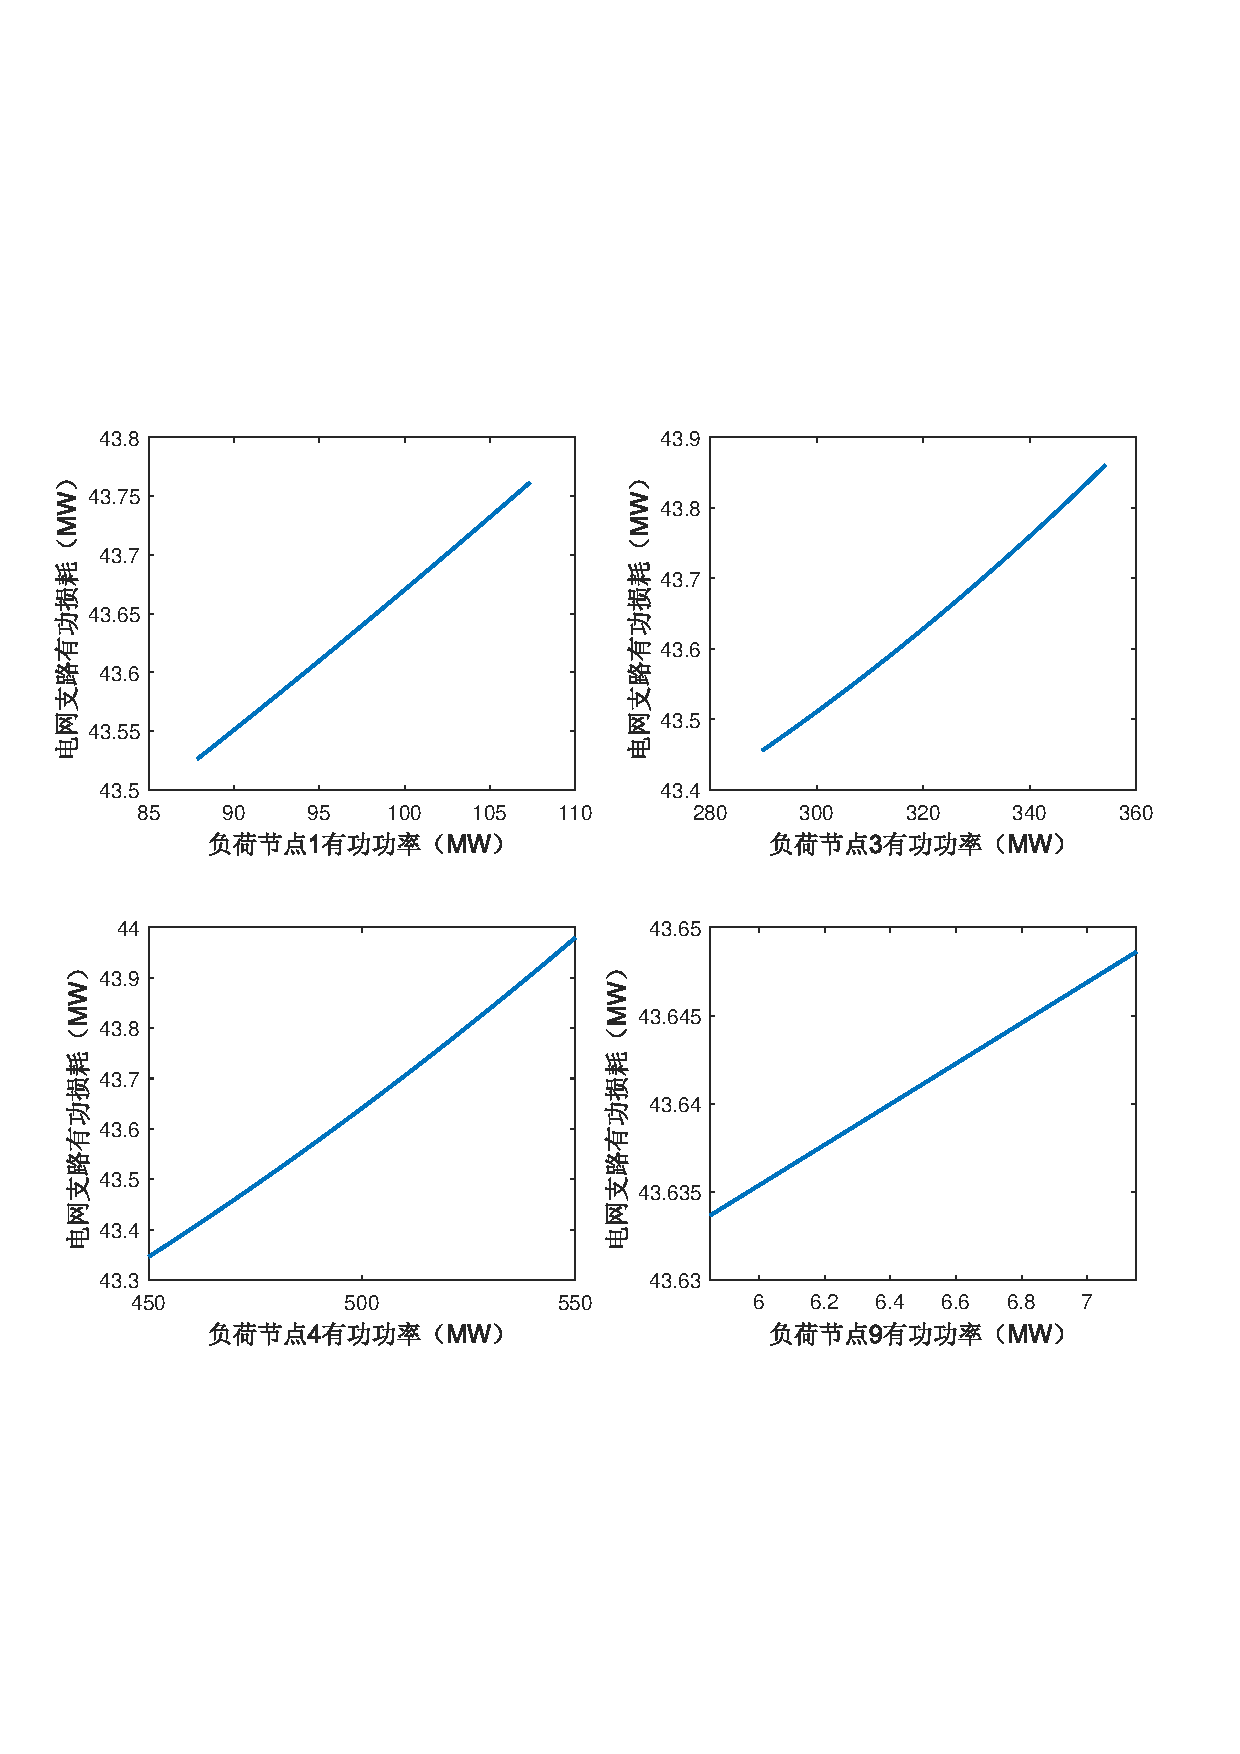
\includegraphics[height=8cm]{senseTest.pdf}
  \caption{$IEEE39$节点1、3、4、9负荷节点灵敏度趋势图}
  \label{fig:senseTest}
\end{figure}

在考虑实际的电网负荷水平的情况下,负荷节点的用电负荷波动不大,故在仿真实验分析时,选取电网负荷节点稳定运行工作点附近的区间进行研究分析,为此,在负荷节点额定功率值的基础上。
取$\pm$10\%的功率区间来进行仿真分析。从图\ref{fig:senseTest}中可以看出,不同节点有功负荷功率的变化对整个系统电网损耗的灵敏度值不同,具体数据如表所示。
\begin{table}[H]
  \centering
  \caption{节点1、3、4、9负荷节点灵敏度值}
  \label{tab:chap3:senseTest}
  \begin{tabular}{C{2cm}C{2cm}C{2cm}C{2cm}C{2cm}}
  \toprule
  \textbf{节点名} & \textbf{节点1} & \textbf{节点3} & \textbf{节点4} & \textbf{节点9}\\
      \midrule
      灵敏度值   & 0.0121     &0.00629       &0.00633     &0.0115 \\
  \bottomrule
  \end{tabular}
  \end{table}

从上表\ref{tab:chap3:senseTest}节点灵敏度数据可以看出,不同节点的灵敏度值差别很大,说明不同负荷节点的在用电负荷变化的情况下,对电网支路的整体损耗不同。根据潮流计算量化结果,
节点1、9、20、23、25、28、29的灵敏度值较大,从网络拓扑位置上看,这些节点大都接近发电节点,从实验结果可以推断出,发电节点向负荷节点的潮流传输线路中,距离发电节点进的负荷节点,在额定
功率平衡点附近的负荷变化对电网支路损耗的影响较大。就灵敏度指标而言,从侧面反映出系统节点的状态脆弱性与系统结构拓扑有一定的联系。




\section{本章小结}
\label{sec:sum3}






\chapter{电力系统脆弱性指标分析与综合评价模型}
\label{cha:quanti}

\section{引言}
\label{sec:index4}
在上一章中,通过对电力系统脆弱性的本质及脆弱过程进行研究分析,将电力系统的脆弱性分为结构脆弱性和状态脆弱性两个方面。结构脆弱性侧重于某一单元或某些单元退出后,
系统受影响的程度,考察的是某个单元在网络拓扑中的影响程度;状态脆弱性专注于系统的元件在扰动作用下,元件运行状态偏离正常状态的程度,考察的是系统的抗干扰能力。

为了对电力系统的脆弱性进行量化评估,得到脆弱性量化评估结果,基于上一章对结构和状态脆弱性指标的研究分析,分别针对结构脆弱性和状态脆弱性进行脆弱性评价指标的选取,
本章的研究重点在于脆弱性指标选取和多指标融合,建立系统脆弱性量化评估模型,进一步解决系统脆弱性系统脆弱性难以量化的问题,为下一章分析电力系统脆弱性问题,识别系统
脆弱环节奠定了理论基础。

\section{系统脆弱性量化评估指标}
\label{sec:describIndex}
为综合评价系统在扰动后所表现出的脆弱性,建立系统的量化评估模型,需要选取客观合理的系统脆弱性评判指标,并对指标进行分析描述,形成系统脆弱性综合评估指标集结构。



\subsection{电力系统的脆弱性指标选取}
\label{sec:pickIndex}
根据第三章对电力系统脆弱性的研究,将系统的脆弱性分为结构脆弱性和状态脆弱性。因此,本章将从这两个方面分别选取相应的系统脆弱性量化评价指标。

$(1)$结构脆弱性指标$I_1$:

对于结构脆弱性的评价来说,考察的是某一节点或线路因故障退出后对系统结构完整性的影响程度。对于系统结构影响程度大的节点或线路,说明其对网络拓扑结构的完整性贡献程度高,
对于这样的节点或线路称为系统结构的脆弱点。因此我们选取以下指标:

结构指标1:

在复杂网络理论中,度是网络特征的关键参数,描述的是节点的连接情况,表现出节点在结构拓扑中的重要程度。为评估系统节点在结构拓扑中的重要程度,选取电气度作为结构
脆弱性指标:$I_{11} = e_{i}$。

结构指标2:

基于复杂网络理论将系统拓扑等效为一个无向图,在描述网络特征的参数中,介数作为关键参数之一,被描述节点或边在信息、能量传递中的重要程度。为评估系统拓扑在能量传输分
布中的贡献,第二个结构脆弱性指标选为电气介数:$I_{12} = C_B(k)$。

结构指标3:

基于复杂网络理论中的$PageRank$算法,将结构拓扑中的支路潮流方向视为有向图,描述了节点之间的连接关系在系统拓扑的能量传递中的影响程度。第三个结构脆弱性指标选为$PR$值:
$I_{13} = PR(p_i)$。

$(2)$状态脆弱性指标$I_2$:

对于状态脆弱性的评价来说,考察的是在扰动作用下系统节点维持在稳定运行状态的能力,即系统抗干扰的能力,系统节点节点越容易到达临界失稳状态,说明节点的脆弱程度越高。
为了描述系统的当前状态与临界失稳状态的偏离程度,我们选取以下指标:

状态指标1:

电压作为评价电力系统安全稳定运行的重要指标。在电力系统运行过程中,通过比较节点实际的运行电压和临界电压之间的裕度来评估电网各节点的状态脆弱性,因此选取“电压裕度”指标
作为第一个状态脆弱性指标,考虑在概率负荷模型的情况下,基于蒙特卡洛模拟潮流计算的方法对电压裕度指标进行计算:$I_{21} = S_V$。

状态指标2:

通过上一章的状态脆弱性指标研究,通过连续潮流(CPF)计算各节点的临界负荷功率,该指标可以衡量节点所能承受的最大负荷能力,这有利于对负荷进行合理的规划分配。因此,选取
“功率稳定裕度”指标作为第二个状态脆弱性指标:$I_{22} = S_C$

状态指标3:

在电力系统脆弱性研究中,电力系统损耗也是需要重点考虑的一个方面,因此,选取“电网损耗灵敏度”指标第三个状态脆弱性指标:$$I_{23} = S_P = \frac{d P_{LOSS}}{d P_i}$$



\subsection{脆弱性量化评估指标的分析描述}
\label{sec:wordIndex}
电力系统结构脆弱性指的是电网在扰动作用下,保持其连通性和拓扑结构完整性的能力。其结构脆弱性指标描述的是节点在电力系统中的重要程度,本文认为对网络拓扑的完整性和连通性
贡献程度越高的节点,其脆弱程度越高,对电力系统的影响程度也越大。

$(1)$电气度指标:描述的是电力系统的连接情况和连接强度,表征的是系统节点在电力系统拓扑结构中的重要程度。电气度指标的计算是根据电力系统的节点的邻接矩阵和支路的视在功率
得出的,因此,系统节点的电气度指标越大,表示节点在此系统的重要程度越大,其脆弱程度越高。

$(2)$电气介数指标:描述的是电力系统各节点在能量传输分布中的贡献程度。电气介数指标越大,表示节点在能量传输中的贡献程度越高,其在意外扰动下退出时,对系统结构完整性的冲击
较大,其脆弱程度越高。

$(3)$PageRank值指标:PageRank值是基于$PageRank$互联网重要程度排序算法将电力系统等效为无权有向图得到的结构脆弱性指标,具体表现各节点在电力系统潮流传输方向上的能量累计。在潮流累计
分布中贡献程度高的节点,节点PageRank值越大,说明节点脆弱性越高。

电力系统状态脆弱性指的是系统在外界扰动或内部故障后,节点或支路的状态量向临界值逼近的特性。本文认为,在扰动作用下,电力系统中的节点或线路的运行状态值越接近临界失稳值,
其脆弱程度越大,越易影响系统的正常运行。

$(1)$电压裕度指标:电压是衡量电能质量的重要指标,在电力系统运行中,保证系统节点电压的稳定可以有效提高电力系统的运行效率,降低系统出现级联故障的可能性。在电压裕度指标的
计算中,我国规定。300$KV$及以上的母线,正常运行电压不得超过系统额定电压的10$\%$,因此电压偏差率取10$\%$,基于负荷功率模型的基础上,通过蒙特卡洛模拟试验方法,考察在负荷
变化的情况下,系统节点电压状态量的变化。通过电压裕度表达式可知,电压裕度指标值越小,其电压值越接近临界电压值,系统节点的脆弱程度越大。

$(2)$功率稳定裕度指标:描述的是系统节点所能承受的最大负荷量。在电力调度方面有利于合理调配负载,防止系统节点因过载而导致的电网故障。在指标计算方面,本文采用连续潮流(CPF)
计算得到各节点的最大有功负荷功率,进而得到各节点有功功率稳定裕度指标值。

$(3)$电网损耗灵敏度指标:描述的是系统各节点分别在负荷变化下对电网整体损耗的影响程度。这有利于识别出导致电网损耗率较高的关键元件,对降低电网损耗率具有参考价值。在指标计算方面,
考虑的是各节点的有功功率在额定值的$\pm 10 \%$范围内,按指定步长增加负荷,经过不断的潮流计算得到电网整体损耗值,进而得到系统的电网损耗灵敏度。因此,系统节点的灵敏度值越大,
节点的负荷变化对电网损耗越大,对电网元件的损耗越大,进而影响电网的整体运行状态。

本文在指标值处理上,采用“效益型”指标,指标值愈大愈好,具体指的是系统节点的指标值愈大,对电力系统的重要程度愈大,其脆弱程度愈高。

\subsection{系统脆弱性评估指标集结构及融合方法}
\label{sec:IndexSys}
通过电力系统脆弱性指标的选取和分析描述,电力系统的脆弱性评估指标分为结构脆弱性指标和状态脆弱性指标,从两个方面为各自部分脆弱性量化评估的依据。在一级结构指标中有电气度、电气介数
和PR值三个二级结构指标;在一级状态指标中有电压裕度、功率稳定裕度和电网损号灵敏度三个二级状态指标。整体的脆弱性评估指标集结构如图\ref{fig:index}所示。

\begin{figure}[H] % use float package if you want it here
    \centering
    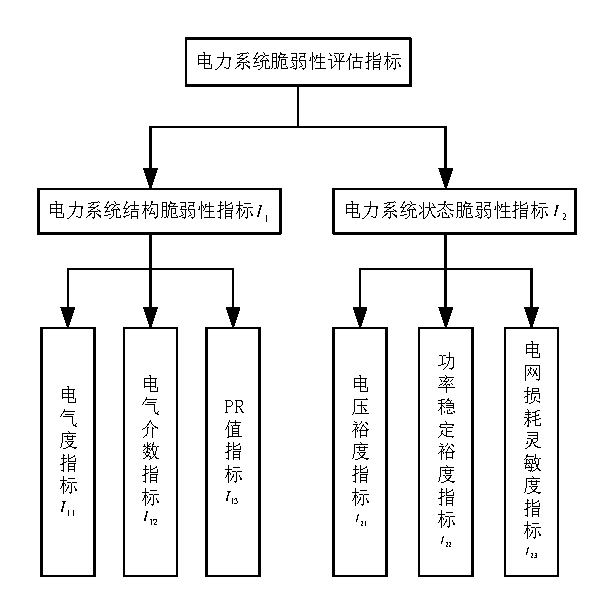
\includegraphics[]{index.pdf}
    \caption{电力系统脆弱性评估指标集}
    \label{fig:index}
  \end{figure}

针对多指标融合方法已有不少研究,在本文第一章绪论中,针对脆弱性评价指标建立系统评价模型的综述中提到,在指标融合方面,指标权重的确定方法主要分为主观法和客观法两类,主观法主要有专家调查法、
环比评分法、层次分析法等;而客观法主要有熵权法、基于方案满意度法 、基于方案贴近度法等。

主观赋权法是在权重分配方面研究较早、较为成熟的方法,其优点在于指标分析者可根据实际的决策问题和实际的知识经验合理地确定各指标的权重,避免出现权重分配结果与实际重要程度相悖的情况。但其缺点
也是相当明显,其评价结果具有较强的主观性,对指标分析者的水平要求较高,依赖于指标分析者的研究水平自身经验,同时增加了专家和决策分析者的研究负担,甚至出现决策偏差较大的情况,在实际应用中存在
很大的局限性。在主观赋权法中,层次分析法是应用最为成熟和广泛的赋权法之一,其在决策分析方法中的简洁实用、所需定量数据少的优点是使其广泛应用的主要原因。但其缺点也不能忽视,当指标过多时,对
决策者的科研水平和自身经验要求提高,主观成分过多,与此同时造成的数据统计量增大,权重难以确定,特征值和特征向量的精确求法也比较复杂。除此之外,根据检验对照表进行矩阵一致性检验,其权重确定
方法缺乏理论证明,其科学合理性不能充分令人信服。


客观赋权法是指单纯利用指标的客观信息而确定权重的方法,在结构脆弱性指标中,电气度、
电气介数和PageRank值这三个指标分别是从三个不同的方面进行研究提出的,对于研究分析者来说,无法从主观来判断其对评价结果的重要程度。另外,三个状态脆弱性指标也是分别从电压稳定性、最大负荷水平
和电网损耗三个角度来进行研究分析的,运用主观分析法进行权重分配,其方案的理论可信度不高,极有可能造成分配结果与实际情况不符,而客观赋权法其判断结果不依赖于人的主观判断,有较强的数学理论依据,
概念清楚,含义明确。

基于以上对主客观赋权法的分析,本文采用客观赋权的方法对电力系统结构和状态两个方面的脆弱性指标进行权重分配,仅根据各节点指标值的数据特点和分布进行权重分配,具有较强的数学理论支撑,不具有主观
随意性,可信度高。


\section{脆弱性量化评估二级指标融合方法研究}
\label{sec:processIndex}
从上述指标集结构来看,系统的二级指标是按照系统结构和状态划分的,从不同角度反映系统的脆弱性特征。针对所选取的结构和状态脆弱性评判指标,需要分别对其状态和结构脆弱性指标集进行融合,
首先要对各个二级指标进行归一化处理,消除量纲级的差异,选取并改进指标融合方法对指标进行权重分配,最后得到结构和状态一级评估指标。


\subsection{脆弱性量化评估指标数据归一化处理}
\label{sec:nomalzMethod}
针对基于不同理论和算法得出的脆弱性评估指标数据,不同指标数据在量纲和数量级上会存在差异。为了对系统节点进行脆弱性评估和指标融合,首先需要对指标数据进行归一化处理,数据的归一化方法
有很多,需要根据不同的数据格式和数据分布采取不同的归一化方法。下面对常用的归一化方法汇总如表\ref{tab:chap4:normalize}所示。
\begin{table}[H]
  \centering
  \caption{数据归一化方法汇总 }\label{tab:chap4:normalize}
  \begin{tabular}{C{3.8cm}C{2.9cm}C{2.7cm}C{3cm}}
  \toprule
  \textbf{方法} & \textbf{适用情况} & \textbf{特点} & \textbf{表达式}\\
        \midrule
        %\tabincell{c}{}
          \tabincell{c}{离差标准化\\(Min-max Normalization)}
           & 适用于最大最小值明确不变的数据      & 不改变数据的原始分布      & $x^{\ast}=\FS{x-x_{min}}{x_{max}-x_{min}}$   \\
  
         z-score~标准化       & 适用于最大值最小值未知的情况,且数据接近正态分布
                                          & 改变数据的原始分布,对离群点规范化效果好            & $x^{\ast}=\FS{x-\mu}{\sigma}$       \\
  
        Logistic~标准化       & 适用于对长尾分布的数据作分段操作
                                          & 改变数据的分布情况             & $x^{\ast}=\FS{\ln x}{\ln n_{max}}$       \\
  
        \tabincell{c}{小数定标标准化\\(Decimal scaling)}    & 适用于数据初期探索,不消除数据属性间权重差异
                                         & 不改变数据分布                      & $x^{\ast}=\FS{x}{10j}$       \\
  
        排序归一化             & 适用于对数据的具体值并不关心,更关心相对排序的数据
                                         & 原始数据变为直线分布            & $x^{\ast}=\FS{x_{rank}}{num_{total}}$       \\
  
        分段归一化             & 适用于数据分布有明显分段特征的情况
                                         & 不改变分段数据的分布            & 根据不同数据段,采用不用方法       \\
  \bottomrule
  \end{tabular}
  \end{table}

通过对数据归一化方法的整理与分析,针对指标集中的各项指标,采取合理的归一化方法将原始数据映射到$\left[0,1\right]$区间内,从而消除了数据之间的量纲和数量级的差异。

根据上节对量化评估脆弱性指标的分析描述,结构脆弱性的电气度、电气介数和PageRank值指标数据是根据复杂网络理论提出的,状态脆弱性的电压裕度、功率稳定裕度和电网损耗灵敏度指标
是根据裕度和灵敏度相关方法提出的,计算得到的指标数据其分布是可以真实反映各节点在系统中的重要程度。为了更好地衡量各节点在电网中的脆弱程度,不改变指标数值的原始分布。
本文在指标数据归一化处理上采用离差标准化方法。

采用离差标准化归一化方法时,需要明确知道数据的上限值和下限值,考虑到电气度、电气介数、PageRank值和电网损耗灵敏度指标无明确的上下限值,加之本文主要评估的是一个系统内各节点
的脆弱程度,所以本文选取同一指标下节点最大和最小指标值分别最为离差标准化的最大和最小值,这样不仅明确了数据的上下限,又不改变原始数据分布,真实反映各节点在系统中的重要程度。

归一化后的各节点的指标值均在$\left[0,1\right]$之间,因此得到归一化后的结构脆弱性指标向量$I_1$和状态脆弱性指标$I_2$。
\begin{equation}
  \left\{\begin{array}{l}{I_{1}=\left[\begin{array}{lll}{I_{11}^{*}} & {I_{12}^{*}} & {I_{13}^{*}}\end{array}\right]} \\
   {I_{2}=\left[\begin{array}{lll}{I_{21}^{*}} & {I_{22}^{*}} & {I_{23}^{*}}\end{array}\right]}\end{array}\right.
  \end{equation}

  
\subsection{基于改进熵权法的权重分配}
\label{sec:nomalz}
在复杂系统理论中,认为复杂系统具有异质性,复杂系统的异质性是指系统中各元件对整体影响程度的不均衡性。在电力系统中,各节点
对系统整体结构的影响程度体现在结构脆弱性指标值上,节点指标值越大,说明节点在系统结构拓扑中的重要性高,对系统整体的影响越大,其脆弱程度越高。
因此,本文认为,系统各节点的脆弱程度的差别是造成电力系统结构脆弱异质性的根本原因。
当系统各节点在某一指标下的指标值大致相近,说明各节点对系统的影响程度相近,进而无法分析各节点脆弱程度和识别系统脆弱环节,则该指标对综合
评价无参考价值。

熵作为热力学中分子运动无序程度的度量,原本用来反映系统蕴含能量的大小。随后被引入到各领域以表征系统无序程度。当分子均匀分布在整个空间内时,分析运动表现出高度的无序性特征,
系统的熵很大。当分子集中于系统中的某一子空间内时,分子运动无序程度很小,系统的熵很小\cite{refs76}。

在信息论中,熵是对信息量的一种描述。熵越大,包含的信息量越小;相反,熵越小,包含的信息量就越大。根据熵的特性,可以通过计算熵值来判断一个事件的随机性及无序程度,
也可以用熵值来描述指标间的差异程度,各指标值间的差别越大,该指标对综合评价的影响(权重)越大。

在结构脆弱性指标集中,每个评价指标是考虑不同节点对电网拓扑结构的影响程度而提出的,所以当指标的熵值越大,说明系统各节点对系统的影响程度比较均衡,
系统的异质性较小;反之,熵值越小,各节点的脆弱性差异也就比较大,系统具有较强的异质性。由于结构脆弱性各指标是从不同方面考虑提出的,不存在信息重合的情况。
所以在评价系统结构脆弱性指标时,基于熵权法的电网结构脆弱性特性分析与评价方法是比较合理的。

本文从熵的角度考虑,认为对于指标数据间差别较大的指标应赋予较高的权重。因此,在对结构脆弱性指标进行融合时,采用并改进熵权法对结构脆弱性指标进行权重分配。

下面对熵权法的步骤进行描述,并对数据处理过程中不合理之处进行改进。

首先,假设有$M$个评价对象,根据综合评估问题的需要,选取$N$个评价指标,计算各评价对象的各指标数值的大小,假设第$m$个评价对象的第$n$个评价指标数值为$\lambda_{mn}$。

然后,由于不同的评价指标在计算结果上存在量纲以及取值范围的差异,所以需要对每个评价指标的数值进行标准归一化处理。其归一化的数值用$\mu_{mn}$表示。

计算各评价指标的熵,表达式如下:
\begin{equation}
\label{equ:chap4:shang1}
  p_{m n}=\frac{\mu_{m}}{\sum_{m=1}^{M} \mu_{m}}
  \end{equation}

\begin{equation}
  H_{n}=-\frac{1}{\ln M} \sum_{m=1}^{M}\left(p_{m n} \ln p_{m n}\right)
  \end{equation}

式\ref{equ:chap4:shang1}中,$p_{mn}$表示第$n$组随机实验中第$m$个随机事件发生的概率(我们假设一个节点对应的指标值越大,其受到扰动或破坏的概率越大);$H_n$表示第$n$个指标的熵。

计算各评价指标的熵权,表达式如下:
\begin{equation}
  w_{n}=\frac{1-H_{n}}{\sum_{n=1}^{N}\left(1-H_{n}\right)}
  \end{equation}

具体映射:在电力系统结构脆弱性评估中,评价对象$M=39$,即1--39节点,评价指标$N=3$,分别为电气度、电气介数和PageRank值,将每个评价指标的数值在评价指标数值总和下所占的比例作为
其所发生的概率$p_{mn}$。

\begin{table}[htb]
  \centering
  \caption{熵权法与电力系统参数映射关系}
  \label{tab:lichaTable1}
    \begin{tabular}{C{5.5cm}C{5.5cm}}
      \toprule
      熵权法参数 & 电力系统参数 \\
      \midrule
      评价对象 &  系统节点 \\
      评价指标 &  结构脆弱性指标 \\
      评价对象概率值 & 节点的指标值占指标总和的比重 \\
      \bottomrule
    \end{tabular}
\end{table}

熵权法的计算流程如图\ref{fig:shang_Procession}所示:
\begin{figure}[H] % use float package if you want it here
  \centering
  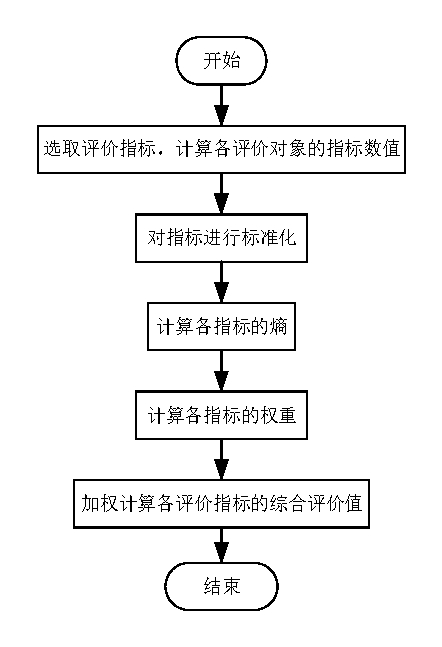
\includegraphics[]{shang_Procession.pdf}
  \caption{熵权法计算流程图}
  \label{fig:shang_Procession}
\end{figure}

在对指标数据进行归一化后,不可避免会出现数值为0的指标值,而熵权法赋权要求指标数据必须全部大于零,否则在取对数计算信息值时,会出现信息值异常的情况。针对这种情况,
传统熵权法的处理方法为:当$p_{mn}=0$,信息值$p_{m n} \ln p_{m n}=0$。这说明脆弱指标值为0的系统节点,其在脆弱程度评价所提供的信息为0,对脆弱性综合评价不起作用。
而在实际的电力系统脆弱性分析中,虽然有的节点在某一脆弱性指标下的指标值极小,但实际却在电网结构和运行中承担极大的作用。其次,其$p_{mn}=0$的信息值与$p_{mn}=1$的
信息值相等,因此,在电网脆弱性指标权重分配处理上,这种方法是不合理的。

为此,考虑到电力系统节点的潜在脆弱性特征,避免在数据处理过程中出现异常,保证数据的完整性和评价的可靠性。本文在不改变指标数据的原始分布的前提下,将结构脆弱性指标归一化
到$[0.002,0.998]$区间内。在对指标数据进行变换后,现有数据会与原始数据有所偏差,本文将其定义为信息损失,除此之外,本文还将对信息损失进行度量,比较指标数据变换前后各指
标数据与均值的偏离程度来量化信息损失,即用方差来定义
信息损失度$\beta$:
\begin{equation}
  \label{equ:chap4:infoloss}
\sum_{i=1}^{n}\left(\mu_{i}^{*}-\bar{\mu}_{i}^{*}\right)^{2} /\sum_{i=1}^{n}\left(\mu_{i}-\bar{\mu}_{i}\right)^{2} \geq 1-\beta 
\end{equation}

式\ref{equ:chap4:infoloss}中,称$\mu_{i}^{*}$为在信息损失度为$\beta$下的指标数据,$\mu_{i}$为原始指标数据。

根据上述改进熵权法,可计算得到在信息损失度为$\beta=0。008$下的结构脆弱性评价指标的权重向量$W$为:
\begin{equation}
\label{equ:chap4:shang2}
   W_1 = \left[w_{1}\ w_{2}\ w_{3}\right]=[0.33\ 0.41\ 0.26]
\end{equation}



\subsection{基于离差最大化法的权重分配}
\label{sec:nomalz}
在状态脆弱性指标研究方面,本文从节点电压稳定性、节点最大负荷功率和电网损耗方面考虑分别提出了电压裕度、功率稳定裕度和电网损耗灵敏度指标来进行电力系统状态脆弱性研究。
在状态脆弱性指标的权重确定方面,本文认为在某一状态指标下,电网各节点的状态指标值是不同的,当电力系统各节点的状态指标值的差别很小时,说明选取的指标在电力系统的量化评估中起到的
作用很小,应赋予小的权重,这在一定程度反映一个问题,这就是为什么我们在选取评价指标时,要从不同方面考虑,做的全面客观地选取指标。当电力系统各节点的状态指标值离散程度
大时,说明选取的指标使各节点的状态值产生了很大的变化,不同节点在此指标下的状态值差别很大,说明选取的指标在电力系统的量化评估中起到的作用很大,应赋予较大的权重。

本文将状态脆弱性指标权重分配的问题与多属性决策相联系,采用在多属性决策领域常用权重分配方法--离差最大化法进行状态指标的权重分配,离差最大化的基本思想,量化描述在指标$i$下,
各方案的指标值的离散程度,其表征的意义在于,如果指标$i$对于所有的方案而言,各方案的指标值$u_{ij}$均无差别,那么指标$i$对方案决策与排序将不起作用,这样的评价指标可令其权重系数为0;
如果$i$ 指标能使决策方案的指标值$u_{ij}$间的有较大差异,这样的评价指标对方案决策与排序将起重要作用应该给予较大的权重系数\cite{refs77,refs78}。

通过上述的分析可知,本文认为在电力系统状态脆弱性评估方面,在某一指标下,若系统节点间的状态指标值差别很大,说明该指标在电力系统状态评估方面起到很大的作用,应赋予较大的权重。
因此,在状态脆弱性指标融合方面,本文选用离差最大化法对状态脆弱性指标进行权重分配。

在多属性决策方面,对于某个多属性决策问题,设其方案集为$A = \{A_1,A_2 \cdots A_m\}$,属性集为$G = \{G_1,G_2 \cdots G_n\}$,方案$A_i$对属性$G_j$的指标值
记为$y_{ij}\left(i = 1,2,\cdots,m;j = 1,2,\cdots,n\right)$,矩阵$Y = \left(y_{ij}\right)_{m \times n}$表示方案集A对属性集G的“属性矩阵”,俗称“决策矩阵”。
% 通常指标的类型有“效益型”指标、“成本型”指标、“固定型”指标和“区间型”指标。“效益性”指标是指属性值愈大愈好的指标,如资金产值率、人均国民生产总值等;“成本型”指标是指属性值愈
% 小愈好的指标,如流动资金占用额,资金周转天数等;“固定型”指标是指属性值既不能太大又不能太小,而以稳定在某个固定值为最佳的一类指标,家用电器稳压器的稳压性能指标就属于
% 这类指标;“区间型”指标是指属性值以落在某个固定区间内为最佳的一类指标,国家标准中规定的等级划分通常都属于这类指标。
在4.2.2节的脆弱性量化评估指标的分析描述中,本文在指标处理上采用的“效益型”指标,指标值越大越好\cite{refs78}。

对矩阵$Y$进行归一化处理后得到的决策矩阵记为$Z = (z_{ij})_(m \times n)$,显然,$z_{ij}$愈大愈好,设评价指标间的加权向量为$W = [w_1,w_2 \cdots w_n]^T > 0$,并满足
单位化约束条件
\begin{equation}
  \sum_{j=1}^{m} w_{j}^{2}=1
\end{equation}
  
在加权向量$W$的作用下,构造加权规范化决策矩阵
\begin{equation}
C = \left[\begin{array}{cccc}{w_{1} z_{11}} & {w_{2} z_{12}} & {\cdots} & {w_{n} z_{1 n}} \\ {w_{1} z_{21}} & {w_{2} z_{22}} & {\cdots} & {w_{n} z_{2 n}} \\ 
{\vdots} & {\vdots} & {} & {\vdots} \\ {w_{1} z_{m 1}} & {w_{2} z_{m 2}} & {\cdots} & {w_{n} z_{m n}}\end{array}\right]
\end{equation}

根据简单加性加权法(SAW),各决策方案$A_i$的多指标综合评价值可表示为
\begin{equation}
\label{equ:chap4:SAW}
  D_i(w) = \sum_{j = 1}^{n} z_{ij}w_{j} , i=1,2 \cdots n
\end{equation}

可以看出,$D_i(w)$值愈大表明决策方案$A_i$愈优。因此,在加权向量$W$已知的情况下,根据式\ref{equ:chap4:SAW}可以对各决策方案进行决策或排序。下面将求解加权向量$W$.
根据离差最大化的基本思想,对于$G_j$属性而言,存在一组权重向量W,使得决策方案$A_{i}$与其他所有的决策方案的离差最大,其表达式可定义为
\begin{equation}
\begin{aligned} V_{i j}(w) &=\sum_{k=1}^{m}\left|w_{j} z_{i j}-w_{j} z_{k j}\right| \\ i=& 1,2 \cdots m, j=1,2 \cdots n \end{aligned}
\end{equation}

令
\begin{equation}
\begin{aligned} V_{j}(w)=\sum_{k=1}^{m} V_{i j}(w) &=\sum_{k}^{m} \sum_{k=1}^{m}\left|z_{i j}-z_{k j}\right| w_{j} \\ j=1,2 \cdots n \end{aligned}
\end{equation}

则$V_{j}(w)$表示对$G_{j}$而言,所有决策方案与其他决策方案的总离差。根据离差最大化的思想,加权向量$W$的确定应是总离差$V_{j}(w)$最大。为此,构造目标函数为
\begin{equation}
\label{equ:chap4:licha1}
\begin{aligned} \max F(w) &=\sum_{j=1}^{n} V_{j}(w) \\ &=\sum_{j=1}^{n} \sum_{i=1}^{m} \sum_{k=1}^{m}\left|z_{i j}-z_{k j}\right| w_{j} \end{aligned}
\end{equation}

于是,求解加权向量$W$转化为求解式\ref{equ:chap4:licha1}的最大值问题
\begin{equation}
\label{equ:chap4:lichaMode}
\left\{\begin{array}{l}{\max F(w)=\sum_{j=1}^{n} \sum_{i=1}^{m} \sum_{k=1}^{m}\left|z_{i j}-z_{k j}\right| w_{j}} \\ 
{\text { s.t. } \sum_{j=1}^{n} w_{j}^{2}=1}\end{array}\right.
\end{equation}

解此最优化模型\ref{equ:chap4:lichaMode},得到
\begin{equation}
  w_{j}=\frac{\sum_{k=1}^{m} \sum_{k=1}^{m}\left|z_{i j}-z_{i j}\right|}{\sum_{j=1}^{n}\left[\sum_{i=1}^{m} \sum_{k=1}^{m} | z_{ij}-z_{k j} | \right]^{2}}, j=1,2 \cdots n
  \end{equation}

理论上可以证明$W^* = [w_1,w_2 \cdots w_n]^T$为目标函数$F(w)$的唯一极大值点。 在得到单位化加权向量$W^*$后,为了进行权重分配,需要对$W^*$进行归一化处理
\begin{equation}
  \bar{w_{j}} = \frac{w_{j}^*}{\sum_{j=1}^{n} w_{j}^*} , j=1,2 \cdots n  
\end{equation}

由此得到归一化权重向量
\begin{equation}
  \bar{w_{j}}=\frac{\sum_{k=1}^{m} \sum_{k=1}^{m}\left|z_{i j}-z_{i j}\right|}{\sum_{j=1}^{n}\sum_{i=1}^{m} \sum_{k=1}^{m} | z_{ij}-z_{k j}|}, j=1,2 \cdots n
  \end{equation}

本文在运用离差最大化进行状态脆弱性指标融合时,方案集$A_i$对应系统节点名称,属性集$G_j$对应状态脆弱性指标集,方案的属性值对应为系统节点的指标值。其映射关系如表\ref{tab:lichaTable1}
所示:
\begin{table}[htb]
  \centering
  \caption{多属性决策与电力系统参数映射关系}
  \label{tab:lichaTable1}
    \begin{tabular}{C{4.5cm}C{4.5cm}}
      \toprule
      多属性决策参数 & 电力系统参数 \\
      \midrule
      方案集 & 系统节点集 \\
      属性集 & 状态脆弱性指标集 \\
      方案的属性值 & 系统节点的指标值 \\
      \bottomrule
    \end{tabular}
\end{table}

综上所述,运用离差最大化法对状态脆弱性指标进行权重分配的步骤如图\ref{fig:licha_Procession}下:
\begin{figure}[H] % use float package if you want it here
  \centering
  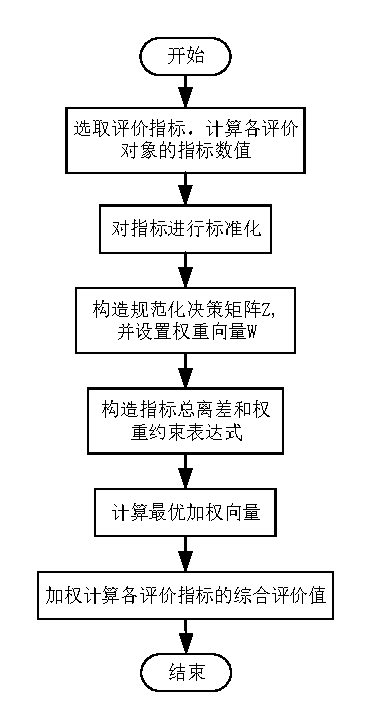
\includegraphics[]{licha_Procession.pdf}
  \caption{离差最大化权重分配流程图}
  \label{fig:licha_Procession}
\end{figure}

根据上述离差最大化原理,计算得到状态脆弱性指标集权重向量$W$如下:
\begin{equation}
  \label{equ:chap4:quanzhong2}
    W_2 = \left[w_{1}\ w_{2}\ w_{3}\right]=[0.29\ 0.34\ 0.37]
    \end{equation}


\subsection{脆弱性量化评估二级指标融合}
\label{sec:2ndIndexMerge}

通过第三章对电力系统脆弱性指标的研究和计算,得到脆弱性指标值后,运用$Matlab$工具实现对结构脆弱性指标和状态脆弱性指标的权重分配,其权重分配结果汇总如下:
\begin{table}[htb]
  \centering
  \caption{二级指标权重分配结果}
  \label{tab:quanzhong3}
    \begin{tabular}{C{3.5cm}C{3.5cm}C{3.5cm}}
      \toprule
      指标类型 & 指标名称 & 权重系数 \\
      \midrule
                    & 电气度  &  0.33 \\
      结构脆弱性指标 & 电气介数 & 0.41 \\
                    & PageRank值 & 0.26 \\
                    & 电压裕度  &  0.29 \\
      状态脆弱性指标 & 功率稳定裕度 & 0.34 \\
                    & 电网损耗灵敏度 & 0.37 \\ 
      \bottomrule
    \end{tabular}
\end{table}

\begin{figure}[H] % use float package if you want it here
  \centering
  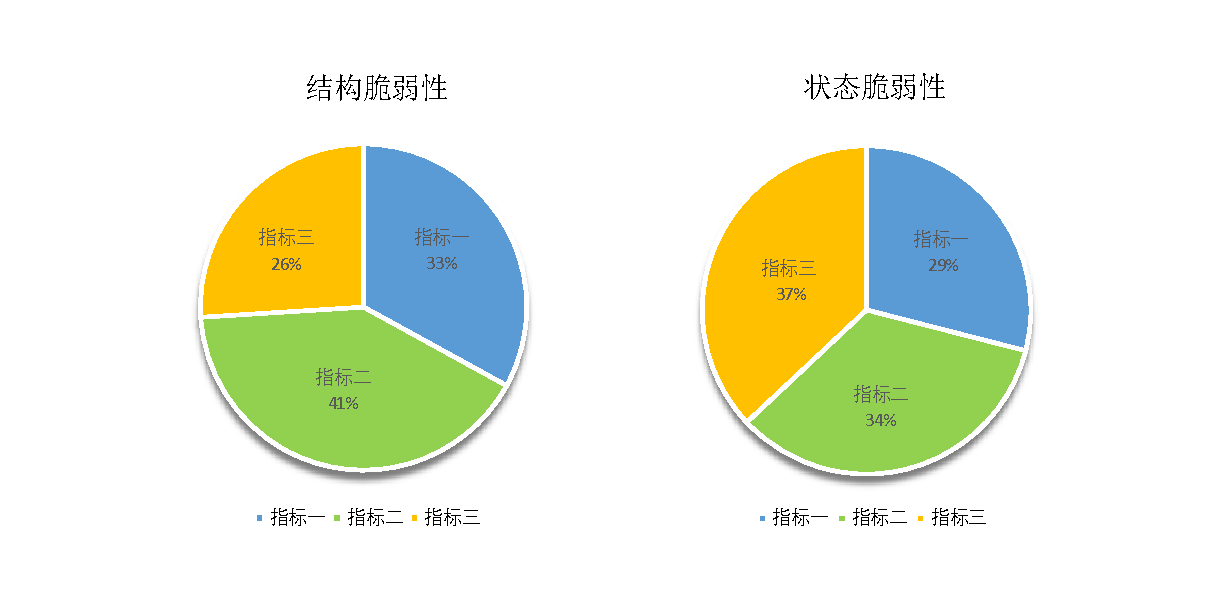
\includegraphics[width=14cm,height=7cm]{quanzhong.pdf}
  \caption{系统二级脆弱性指标权重图}
  \label{fig:quanzhong}
\end{figure}

从图\ref{fig:quanzhong}中可以看出,对于结构脆弱性指标而言,指标二电气介数对于电力系统脆弱性评价影响最大,因为该指标在进行节点重要性分析时,不仅考虑到系统节点在拓扑中的重要性
还考虑到潮流能量分布对结构的影响程度,所以从改进的熵权法的权重结果上,电气介数在脆弱性评估上赋予较大的权重是合理的。对于状态脆弱性指标而言,各指标的权重分配结果差别不大,其中
指标二功率稳定裕度和指标三电网损耗灵敏度所占权重较大,而指标一电压稳定裕度权重最小,其原因在于电力系统各节点的差异性,在指标二和指标三中,两个指标都是各自节点参数的改变来确定各
节点的指标值,如电网损耗灵敏度指标,该指标是通过增加某节点的有功功率经潮流计算得到电网损耗值。指标一不同的是,该指标是运用蒙特卡洛模拟实际电网负荷变化,来计算节点电压的平均电压裕度,
加之电网电压在实际负荷变化情况下,其本身的稳定性较强,电压值变化幅度较小,导致各节点的指标值离散程度较小,所以该指标在最大离差化法的权重计算结果中,所占的权重最小。

因此,本文由权重分配结果对结构和状态的各脆弱性指标进行融合,其表达式如下:
\begin{equation}
\begin{aligned} V_{1} &=I_{1} \cdot W_1^{T} \\ &=\left[\begin{array}{lll}{I_{11}^{*}} & {I_{12}^{*}} & {I_{13}^{*}}\end{array}\right] \cdot\left[\begin{array}{lll}{w_{1}} & {w_{2}} & {w_{3}}\end{array}\right]^{T}, V_{1} \in[0,1] \end{aligned}
\end{equation}
\begin{equation}
\begin{aligned} V_{2} &=I_{1} \cdot W_2^{T} \\ &=\left[\begin{array}{lll}{I_{21}^{*}} & {I_{22}^{*}} & {I_{23}^{*}}\end{array}\right] \cdot\left[\begin{array}{lll}{w_{1}} & {w_{2}} & {w_{3}}\end{array}\right]^{T}, V_{2} \in[0,1] \end{aligned}
\end{equation}


\section{脆弱性量化评估一级指标融合}
\label{sec:DS}
经过上节的研究分析得到了结构和状态两个独立的评判指标$V_1$和$V_2$,将这两个一级指标进行融合是本节研究的重点,本文用概率统计的方法对系统的脆弱程度进行评估,也就是将系统的脆弱性事件分为两类:
脆弱和非脆弱,考虑到事件和一级指标间的独立性,本节基于D-S证据理论,对一级指标进行融合,最终得到一个$0-1$范围内的系统脆弱性综合评价结果。

\subsection{D-S证据理论}
\label{sec:DStheory}
D-S证据理论是最早由Dempster提出,后由Shafter进行补充的用于处理不确定性问题的完整理论。其原理是Dempster通过定义命题的不确定性,提出集值映射和上、下限概率的概念,然后给出Dempster法则
作为证据融合规则,最后Shafer引入信任函数重新定义上、下限概率,得出具有普适性的D-S证据理论。D-S证据理论的特点:由贝叶斯理论发展而来,但约束条件比贝叶斯概率理论更弱;采用“区间估计”而非
“点估计”来描述事件的不确定性;不仅能够强调事物的客观性,还能强调人类对事物估计的主观性\cite{refs79}。

\begin{definition}
辨识框架(Frame of Discernment)
\end{definition}
设$\Theta=\left\{\theta_{1}, \theta_{2}, \ldots, \theta_{n}\right\}$,若非空集合$\Theta$是由$n$个互不相容的元素组成,那么称$\Theta$是辨识框架。

在D-S证据理论中,辨识框架表示关于命题的彼此独立的所有答案或假设的有限集合\cite{refs80}。$2^\Theta$是$\Theta$的幂集,表示辨识框架的所有子集(包含空集),
即$2^{\Theta}=\left\{\phi,\left\{\theta_{1}\right\},\left\{\theta_{2}\right\}, \ldots,\left\{\theta_{n}\right\},\left\{\theta_{1}, \theta_{2}\right\},\left\{\theta_{1}, \theta_{3}\right\}, \ldots, \Theta\right\}$。

\begin{definition}
基本概率赋值函数(Basic Probability Assignment)
\end{definition}
设$\Theta$为一识别框架,$A$是$\Theta$上的任意子集,若函数$m$:$2^{\Theta} \rightarrow[0,1]$,满足条件
\begin{equation}
\left\{\begin{array}{l}{m(\emptyset)=0} \\ {\sum_{A \subset \Theta} m(A)=1} \\ {m(A)>0}\end{array}\right.
\end{equation}

称函数$m$是$2^\Theta$上的概率赋值函数。$\forall A \subset \Theta$,$m(A)$为$A$的基本信任值,表示该条证据对命题$A$的支持程度,$m(A)$仅表示对$A$的信任,不反映对其他任何子集的支持度。
其中,使得$m(A)>0$的$A$称为焦元。
\begin{definition}
置信函数(Belief Function)和似真函数(Plausibility Function)
\end{definition}
\begin{equation}
  \operatorname{Bel}(A)=\sum_{B \subseteq A} m(B), \forall A \subseteq \Theta
\end{equation}
\begin{equation}
  \operatorname{Pl}(A)=\sum_{B \cap A \neq \varnothing} m(B)
\end{equation}

上式中,$B$为$A$的子集,函数$Bel$是$\Theta$上的置信函数。对于任一$A \subset \Theta$,$Bel(A)$是对$A$的置信度,表示$A$发生的可能性;函数$Pl$是辨识框架$\Theta$上的似真函数。
对于任一$A \subset \Theta$,$Pl(A)$是对$A$的似真度,表示$A$可能为真的不确定度量。在证据理论中,通常用$\left[Bel(A),Pl(A)\right]$来表示证据对$A$的信任区间。D-S证据理论对于事件A的
不确定性描述如图\ref{fig:undefined}所示。
\begin{figure}[H] % use float package if you want it here
  \centering
  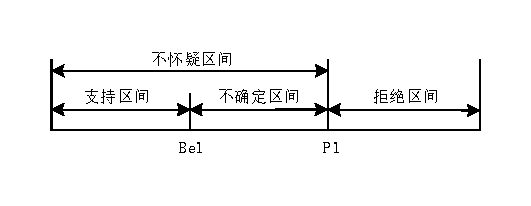
\includegraphics[]{undefined.pdf}
  \caption{对事件A的不确定性描述}
  \label{fig:undefined}
\end{figure}
\begin{table}[htb]
  \centering
  \caption{对命题A各区间的解释}
  \label{tab:undefined}
    \begin{tabular}{C{5.5cm}C{6cm}}
      \toprule
      $\left[Bel(A),Pl(A)\right]$ & 解释描述 \\
      \midrule
      $\left[0,1\right]$ & 对命题A完全不确定 \\
      $\left[0.7,0.7\right]$ & 命题A为真的准确概率为0.6 \\
      $\left[0,0\right]$ & 命题A完全为假 \\
      $\left[1,1\right]$ & 命题A完全为真 \\
      $\left[0.4,0.6\right]$ & 命题A为真的概率在0.4和0.6之间 \\
      \bottomrule
    \end{tabular}
\end{table}

在证据理论的合成规则上,假设$m_1,m_2,\cdots,m_k$分别是同一识别框架$\Theta$上的$k$个基本概率赋值函数,对应的焦元分别为$A_i(i=1,2,\cdots,k)$,设
$K=\sum_{A_{1} \cap \cdots \cap A_{k} = \varnothing } m_{1}\left(A_{1}\right) m_{2}\left(A_{2}\right) \cdots m_{k}\left(A_{k}\right)<1$,若映射$m$:
$2^ \Theta \rightarrow \left[0,1\right]$,则$k$条证据的合成规则为:
\begin{equation}
\label{equ:chap4:rules}
m(A)=\left\{\begin{array}{ll}{0} & {A=\Theta} \\ {\frac{\sum_{A_{1} \cap A_{2} \cap \cdots \cap A_{k}=A} m_{1}\left(A_{1}\right) m_{2}\left(A_{2}\right) \cdots m_{k}\left(A_{k}\right)}{1-K}} & {A \neq \Theta}\end{array}\right.
\end{equation}

式\ref{equ:chap4:rules}中,$K$表示证据间的冲突系数,表示证据间的冲突系数。

式\ref{equ:chap4:rules}融合公式需要满足两个条件\cite{refs81}:
\begin{itemize}
  \item 各证据间互不影响,数据信息相互独立。
  \item 辨识框架中各事件具有互斥性和完备性。 
\end{itemize}

通过研究可以得出,D-S证据理论中不确定性推理流程为:

$(1)$建立辨识框架$\Theta$,确定命题的完备集,生成基本概率赋值函数(BPA);

$(2)$对各证据进行组合,对加入的证据进行概率更新,计算冲突系数$K$;

$(3)$确定计算事件的$Bel$和$Pl$,得到事件置信区间;

$(4)$根据Dempster证据组合规则,计算确定事件的BPA函数;

$(5)$将BPA函数的可信度转换为概率,对融合结果做出决策。

\subsection{脆弱性量化评估一级指标融合}
\label{sec:DSdistri}
在本文中,电力系统脆弱性分结构和状态两方面进行研究,通过客观赋权融合方法分别得到结构指标$V_1$和状态指标$V_2$,这两个指标分别从两个完全不同的方面对系统脆弱性问题展开分析的,
因此,可将这两个一级指标视为两条独立的证据,它们分别从不同方面对系统脆弱性这一不确定性事件进行描述评估。鉴于D-S证据理论是用于处理不确定性问题的完备理论,所以对于电力系统脆弱性
的综合评价问题满足D-S证据理论的约束条件。

由上述分析可知,电力系统脆弱性辨识框架由两个事件构成完备事件集:脆弱和非脆弱。结构脆弱性指标和状态脆弱性指标可作为指向系统脆弱性的两条独立的证据,其中概率赋值函数(BPA)可用指标概率值$P$
表示:
\begin{equation}
\left\{\begin{array}{l}{ V_1 = P_1 \times 100\%} \\ {V_2 = P_2 \times 100\%}\end{array}\right.
\end{equation}

式中指标概率值$P_1,P_2 \rightarrow \left[0,1\right]$。

电力系统脆弱性辨识框架可定义为:
\begin{equation}
  \Theta = \left\{V_{vulnerable},V_{unvulnerable}\right\}
\end{equation}

各证据的基本概率赋值函数(BPA)可定义为:
\begin{equation}
\left\{\begin{array}{l}{m_1(\left\{V_{vulnerable}\right\},\left\{V_{unvulnerable}\right\}) = (V_{1} , 1-V_{1})} \\ 
{m_2(\left\{V_{vulnerable}\right\},\left\{V_{unvulnerable}\right\}) = (V_{2} , 1-V_{2})}\end{array}\right.
\end{equation}

根据D-S证据理论的合成规则,即式\ref{equ:chap4:rules},可得到两指标证据下脆弱事件的BPA值,本文将其定义为脆弱性综合评价指数$E_{vul}$:
\begin{equation}
\label{equ:chap4:vulnerable}
\begin{aligned} E_{vul} &=m(vulnerable) \\ 
 &=\frac{\sum_{X \cap Y=\{\text {vulnerable}\}} m_{1}(X) m_{2}(Y)}{\sum_{X \cap Y \neq \varnothing} m_{1}(X) m_{2}(Y)} \\
 &=\frac{V_{1} \times V_{2}}{V_{1} \times V_{2}+\left(1-V_{1}\right) \times\left(1-V_{2}\right)} \end{aligned}
\end{equation}

式\ref{equ:chap4:vulnerable}中,两条指标证据对应的概率赋值函数分别为$m_1(X)$和$m_2(Y)$,其子集均为$\left\{V_{vulnerable},V_{unvulnerable} \right\}$,脆弱性综合评价指数$E_{vul}$
是由系统结构和状态两方面指标得出,可综合评价电力系统各节点的脆弱程度,脆弱性综合评价指数$E_{vul}$越大,表示节点在系统中的脆弱程度越高,系统越差。

对于脆弱性的不确定性描述问题,在辨识框架中,脆弱(vulnerable)和非脆弱(unvulnerable)构成完备事件集,这两个事件属于对立事件,不存在子集和包含关系,且两指标证据的识别框架完全相同,
$X$和$Y$的子集结构也完全相同,因此,证据的置信函数(Bel)值和似真函数(Pl)值相等,满足表\ref{tab:undefined}中第二种不确定区间的解释。因此,从基本概率赋值函数(BPA)、置信函数(Bel)
和似真函数(Pl)三方面衡量对脆弱事件(vulnerable)的信任程度相同。

\section{系统脆弱性综合评价模型描述}
\label{sec:systemQuan}
在\ref{sec:DS}中,运用了D-S证据理论对结构脆弱性指标和状态脆弱性指标进行融合,得到电力系统各节点的脆弱性综合评价指数。基于以上研究,本节对评价模型的建立研究工作进行系统性梳理和描述。
其评价模型建立流程如图\ref{fig:model_procession}所示。

在第三章中,本文对系统脆弱性研究分两个方面进行,在系统结构脆弱性方面,根据对电力系统结构脆弱性进行定义和数学描述,基于复杂网络理论得到电气度$I_{11}$、电气介数$I_{12}$和PageRank值
$I_{13}$三个结构脆弱性指标。在系统状态脆弱性研究方面,从电压稳定性、节点负荷承受能力和电网损耗三个方面得到状态脆弱性指标,建立了系统节点负荷变化模型,通过蒙特卡洛模拟实验研究节点在
功率负荷变化的情况下,电压裕度$I_{21}$、功率稳定裕度$I_{22}$和电网损耗灵敏度$I_{23}$的变化情况。

在第四章中,首先,将结构脆弱性指标和状态脆弱性指标分别进行归一化处理,消除数量级和量纲间的差异,
得到$I_1 = \left[I^*_{11},I^*_{12},I^*_{13}\right]$和$I_2 = \left[I^*_{21},I^*_{22},I^*_{23}\right]$。然后,在结构方面,采用改进熵权法对系统结构指标进行权重分配得到结构脆弱
指标$V_1$,在状态方面,采用离差最大化法对系统状态脆弱性指标进行融合得到状态指标$V_2$。最后,将结构指标$V_1$和状态指标$V_2$视为独立的两条证据,基于D-S证据理论进行指标融合得到系统各
节点脆弱性综合评价指数。综上研究,本文建立起了电力系统脆弱性量化评价模型。
\begin{figure}[H] % use float package if you want it here
  \centering
  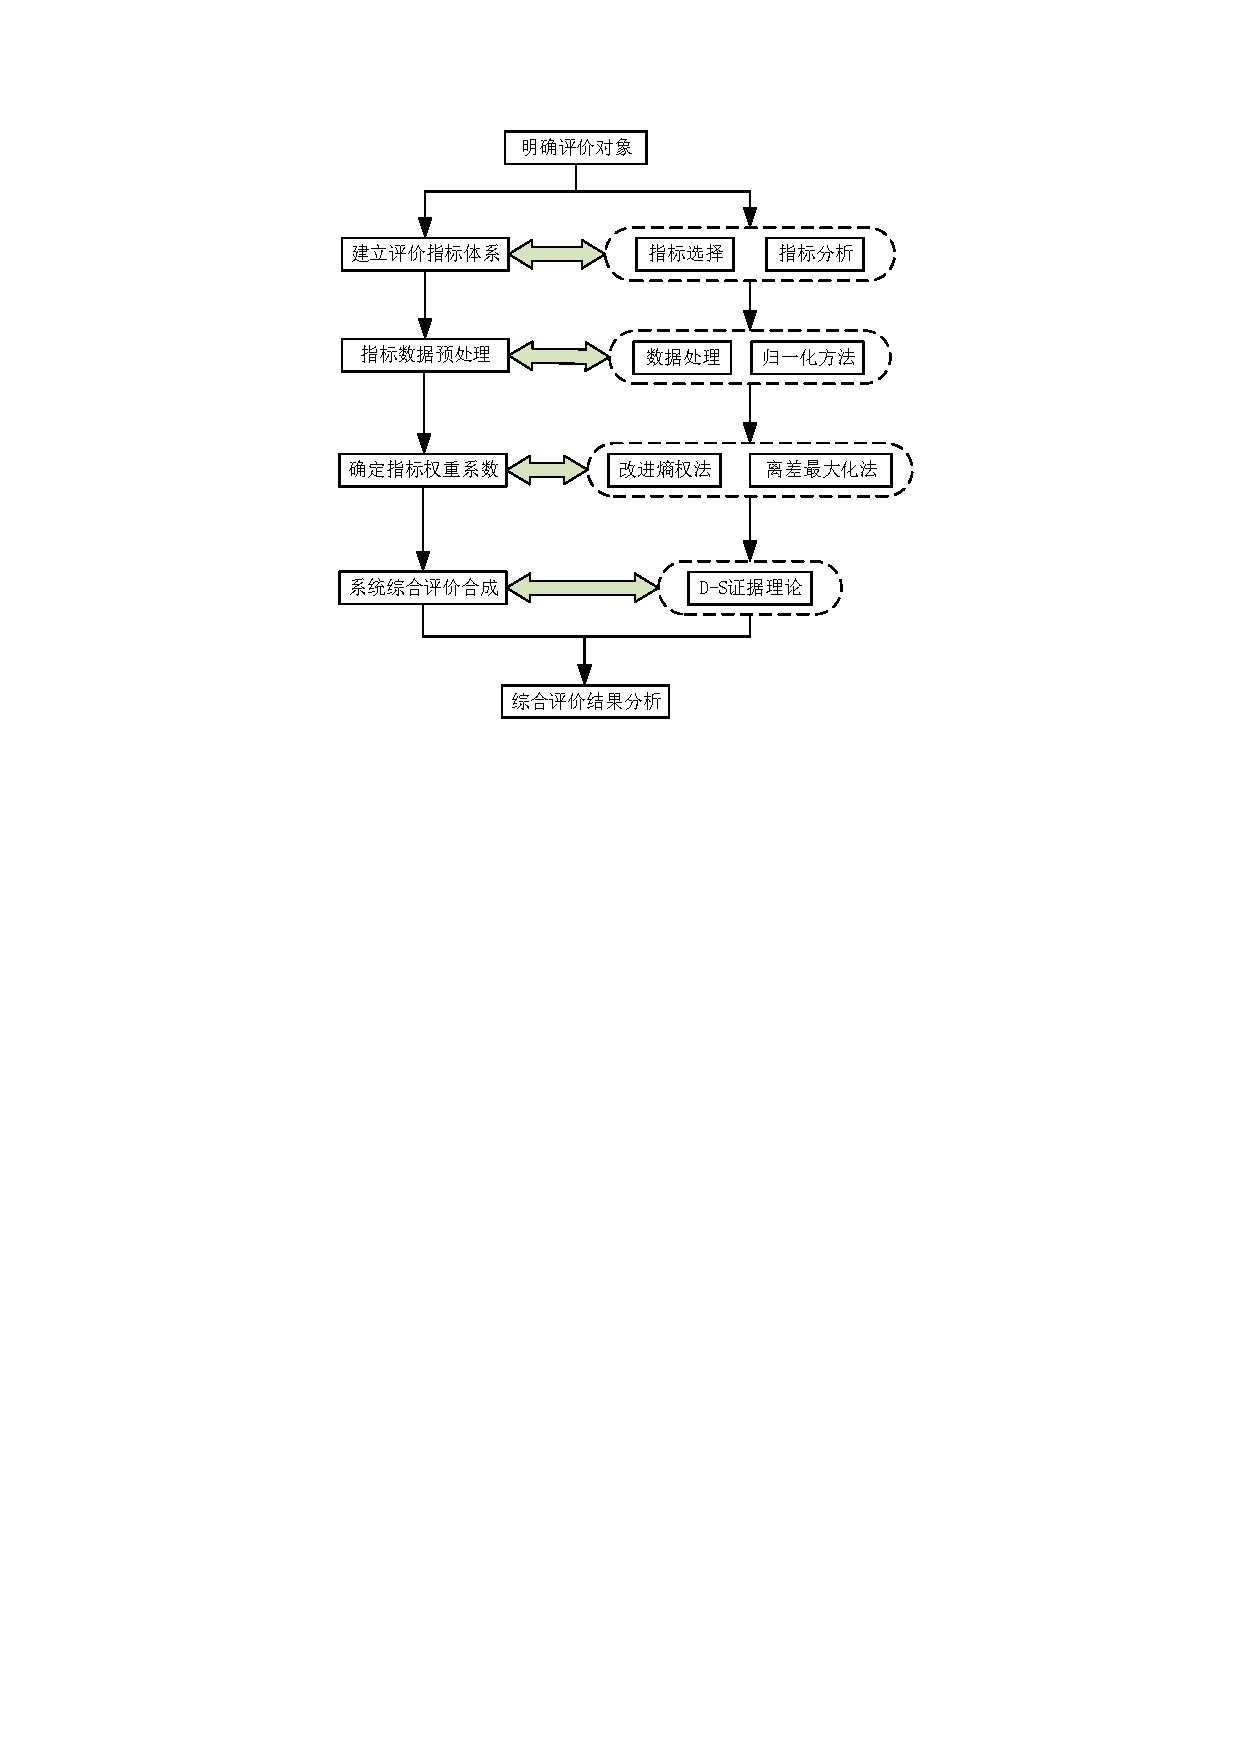
\includegraphics[]{model_procession.pdf}
  \caption{系统脆弱性评价模型流程图}
  \label{fig:model_procession}
\end{figure}


\section{本章小结}
\label{sec:sum4}
本章在系统脆弱性的研究基础上,根据脆弱性的定义与特征,针对结构脆弱性和状态脆弱性分别选取了3个能够反映脆弱性的指标,采用和改进多指标融合方法得到结构脆弱性和状态脆弱性的一级指标。
最后,在$D-S$证据理论的研究基础上,将结构脆弱性指标与状态脆弱性指标进行融合,得到了系统脆弱性综合评价指数,为后文的脆弱性量化分析提供理论基础。




\chapter{电网脆弱性综合评估模型仿真研究}
\label{cha:quantiAnaly}

\section{引言}
\label{sec:index5}
依据第四章所建立的电网脆弱性综合评估模型,
以$IEEE39$标准系统为例,分别进行仿真实验研究电力系统的结构脆弱性和状态脆弱性,分析各节点在系统中的脆弱性,得到系统综合脆弱性评价结果,并对系统脆弱性综合分析。最后,通过基于聚类算法和脆弱性
综合评估结果对系统节点脆弱性等级评估,识别系统的脆弱环节。
% 本章以$IEEE118$标准电网为例,采用静态分析法研究不同攻击策略对电网结构脆弱性的影响,找出最佳的攻击策略,并验证电力系统的网络特性。
% \section{基于复杂网络模型结构脆弱性实验验证分析}
% \label{sec:modelIntroduce}

% \subsection{电网结构脆弱性研究方法}
% \label{sec:modelIntroduce}
% 电网作为一个复杂的人造网络,存在一些固有的缺陷或薄弱环节,当这些薄弱环节遭到破坏时,由于电网节点间的连通性,可能会导致电网运行失稳,引发电网大面积瘫痪。在结构上看,这些缺陷或薄弱环节可视为
% 电网的脆弱环节,因此电网脆弱环节的脆弱程度可以表征电网结构脆弱性。

% 从复杂网络的角度来看,研究电网结构脆弱性的基本方法为通过移除部分节点或线路来考察电网结构和功能的影响程度。电网结构脆弱性的研究方法分为静态分析法和动态分析法,其主要区别在于移除节点或线路
% 后是否考虑所引起的级联反应。静态分析法通过不同的电网攻击策略,分析其对电网结构连通性及传输效率的影响程度,不考虑节点或线路移除后引起的级联反应。动态分析法则考虑的是节点或线路移除后潮流分布
% 变化所引起的级联反应,通过建立连锁故障模型来模拟电网结构性能的动态变化。由于本文对电网结构脆弱性的重点在于识别系统的薄弱环节,选取最优攻击策略,所以在研究方法上,采用静态分析法。 

% \subsection{指标选取及元件攻击策略的制定}
% \label{sec:modelIntroduce}
% 为识别电力系统的脆弱环节并找到最优的攻击策略,需要制定电网的攻击策略以及选取电网整体性能指标,从电网结构拓扑方面考虑,网络传输效率是用于描述电网能量传输的重要性能指标。为此,本文选取第二章所述
% 的网络平均传输效率$E_{mean}$作为电网结构性能评价指标。

% 在第三章中,通过对结构脆弱性的研究,得到电气度、电气介数和$PageRank$值这三个指标作为结构脆弱性指标,为比较这三个指标对于电网结构性能的影响程度,分别按照式\ref{equ:chap3:index1},式\ref{equ:chap3:cb1}
% 和式\ref{equ:chap3:Index3}计算$IEEE118$算例中各节点的电气度、电气介数$PageRank$值,并将各节点的计算结果进行排序。下面将围绕电气度、电气介数$PageRank$值这三个指标指定攻击策略,观察比较
% 电网结构性能指标的变化情况,并引入随机节点攻击策略作为实验对比。具体策略如下:

% $(1)$随机节点攻击策略——每次随机移除1个节点,移除比例为30$\%$,仿真100次,取性能指标结果的平均值;

% $(2)$电气度节点攻击策略——每次移除电气度值最大的节点,移除比例为30$\%$,记录每次的性能指标仿真结果;

% $(3)$电气介数节点攻击策略——每次移除电气介数值最大的节点,移除比例为30$\%$,记录每次的性能指标仿真结果;

% $(4)$$PageRank$值节点攻击策略——每次移除$PageRank$值最大的节点,移除比例为30$\%$,记录每次的性能指标仿真结果;



% \subsection{实验仿真与分析}
% \label{sec:modelIntroduce}
% 本文采用的$IEEE118$标准算例数据见附录A所示,其中各节点电气度、电气介数和$PageRank$值计算结果,分别如图\ref{fig:electricDu118},\ref{fig:nodeBetween118}和\ref{fig:pagerank118}所示,
% 实验结果数据见附录B。
% \begin{figure}[H] % use float package if you want it here
%     \centering
%     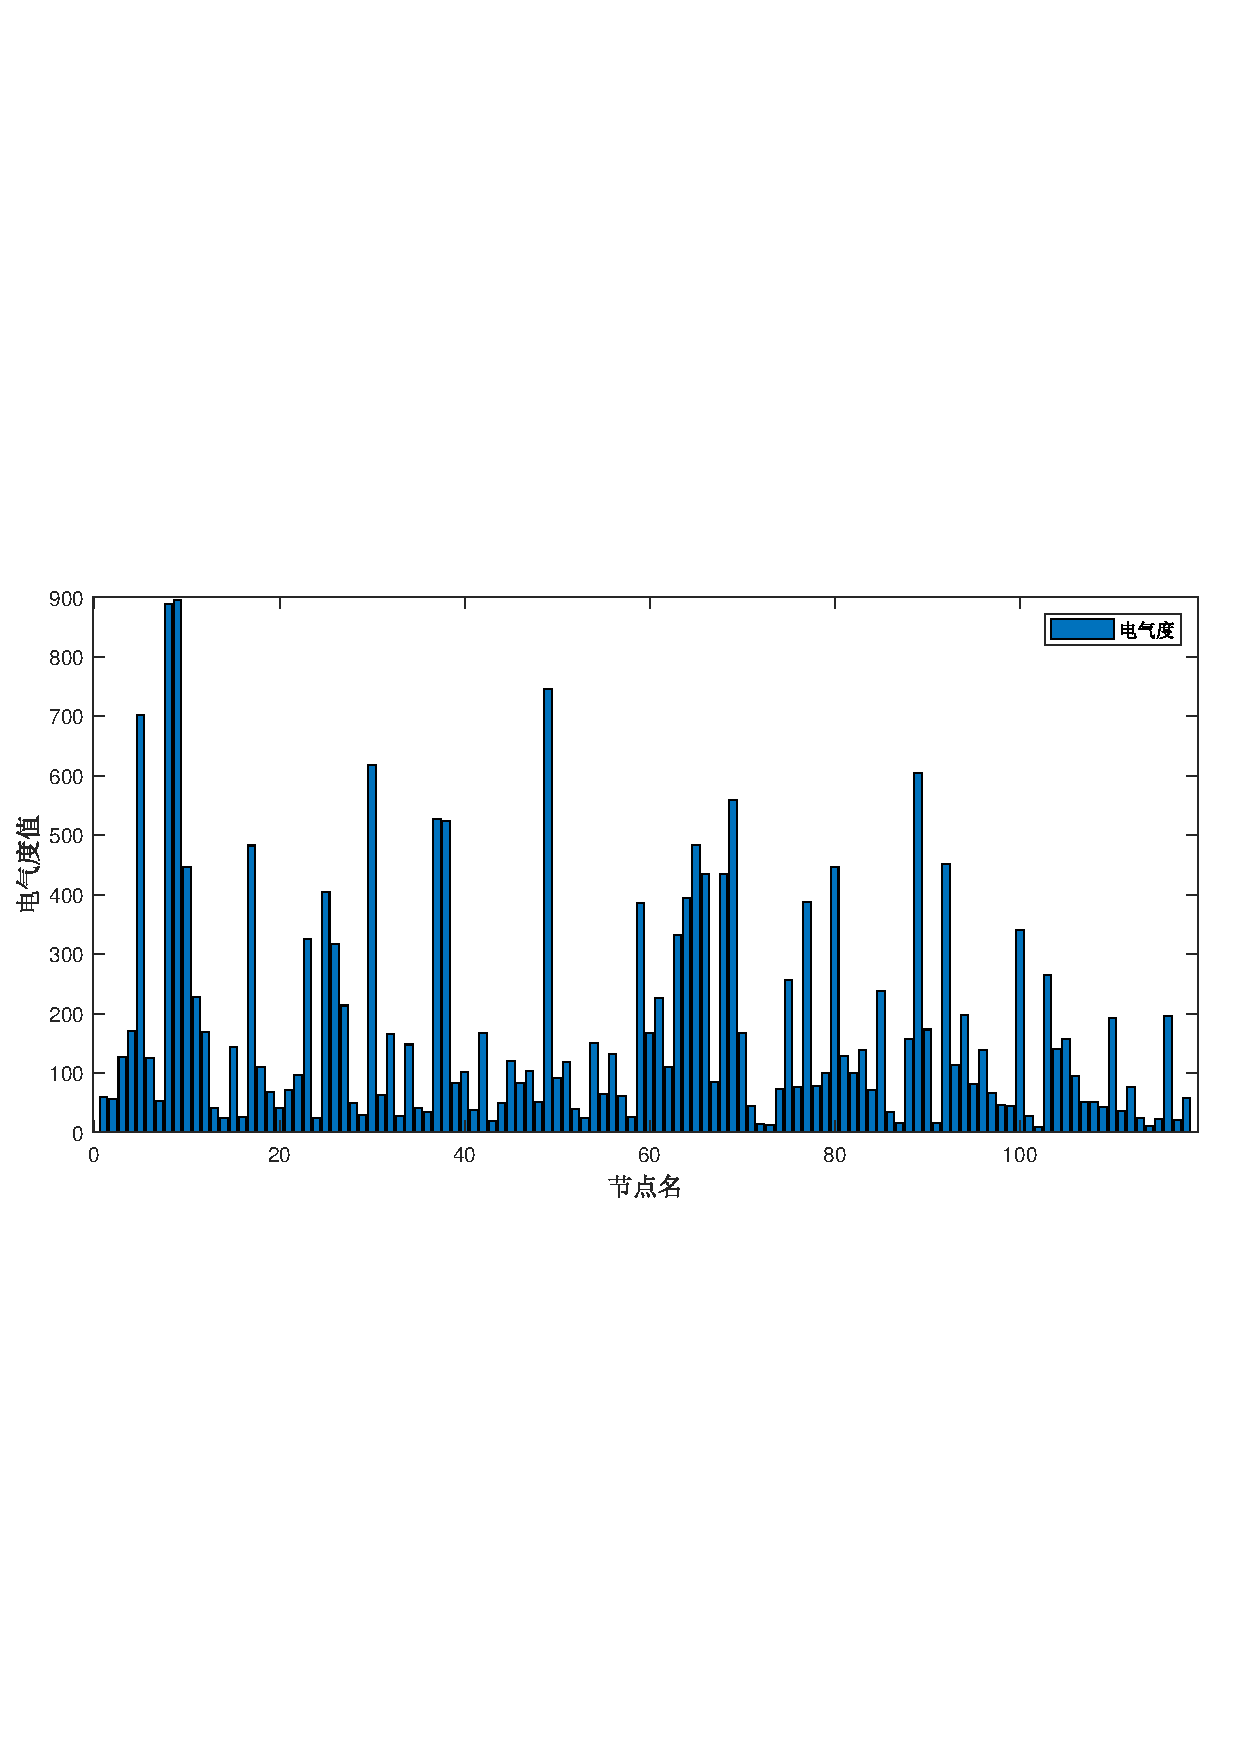
\includegraphics[width=14cm,height=7cm]{electricDu118.pdf}
%     \caption{$IEEE118$节点电气度计算结果图}
%     \label{fig:electricDu118}
%   \end{figure}
% \begin{figure}[H] % use float package if you want it here
%     \centering
%     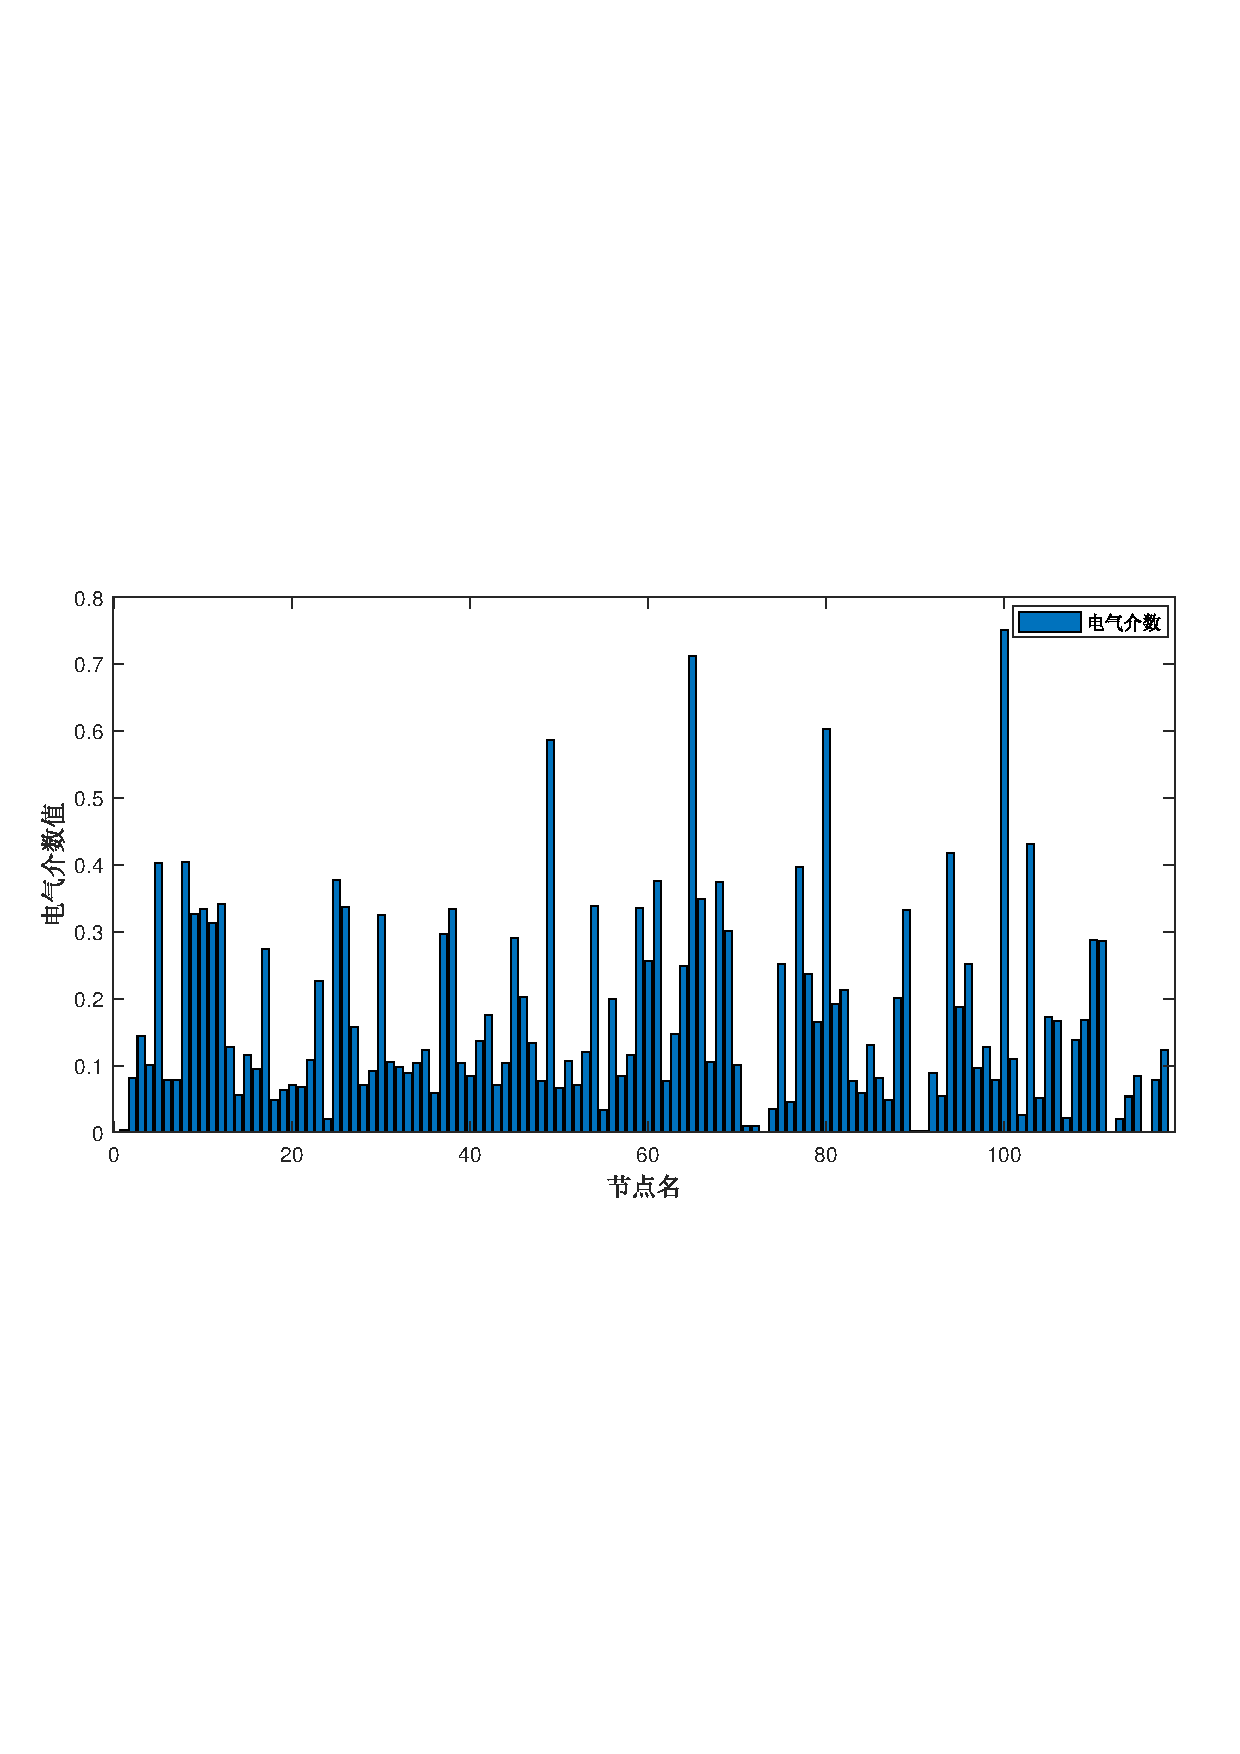
\includegraphics[width=14cm,height=7cm]{nodebetween118.pdf}
%     \caption{$IEEE118$节点电气介数计算结果图}
%     \label{fig:nodeBetween118}
% \end{figure}
% \begin{figure}[H] % use float package if you want it here
%     \centering
%     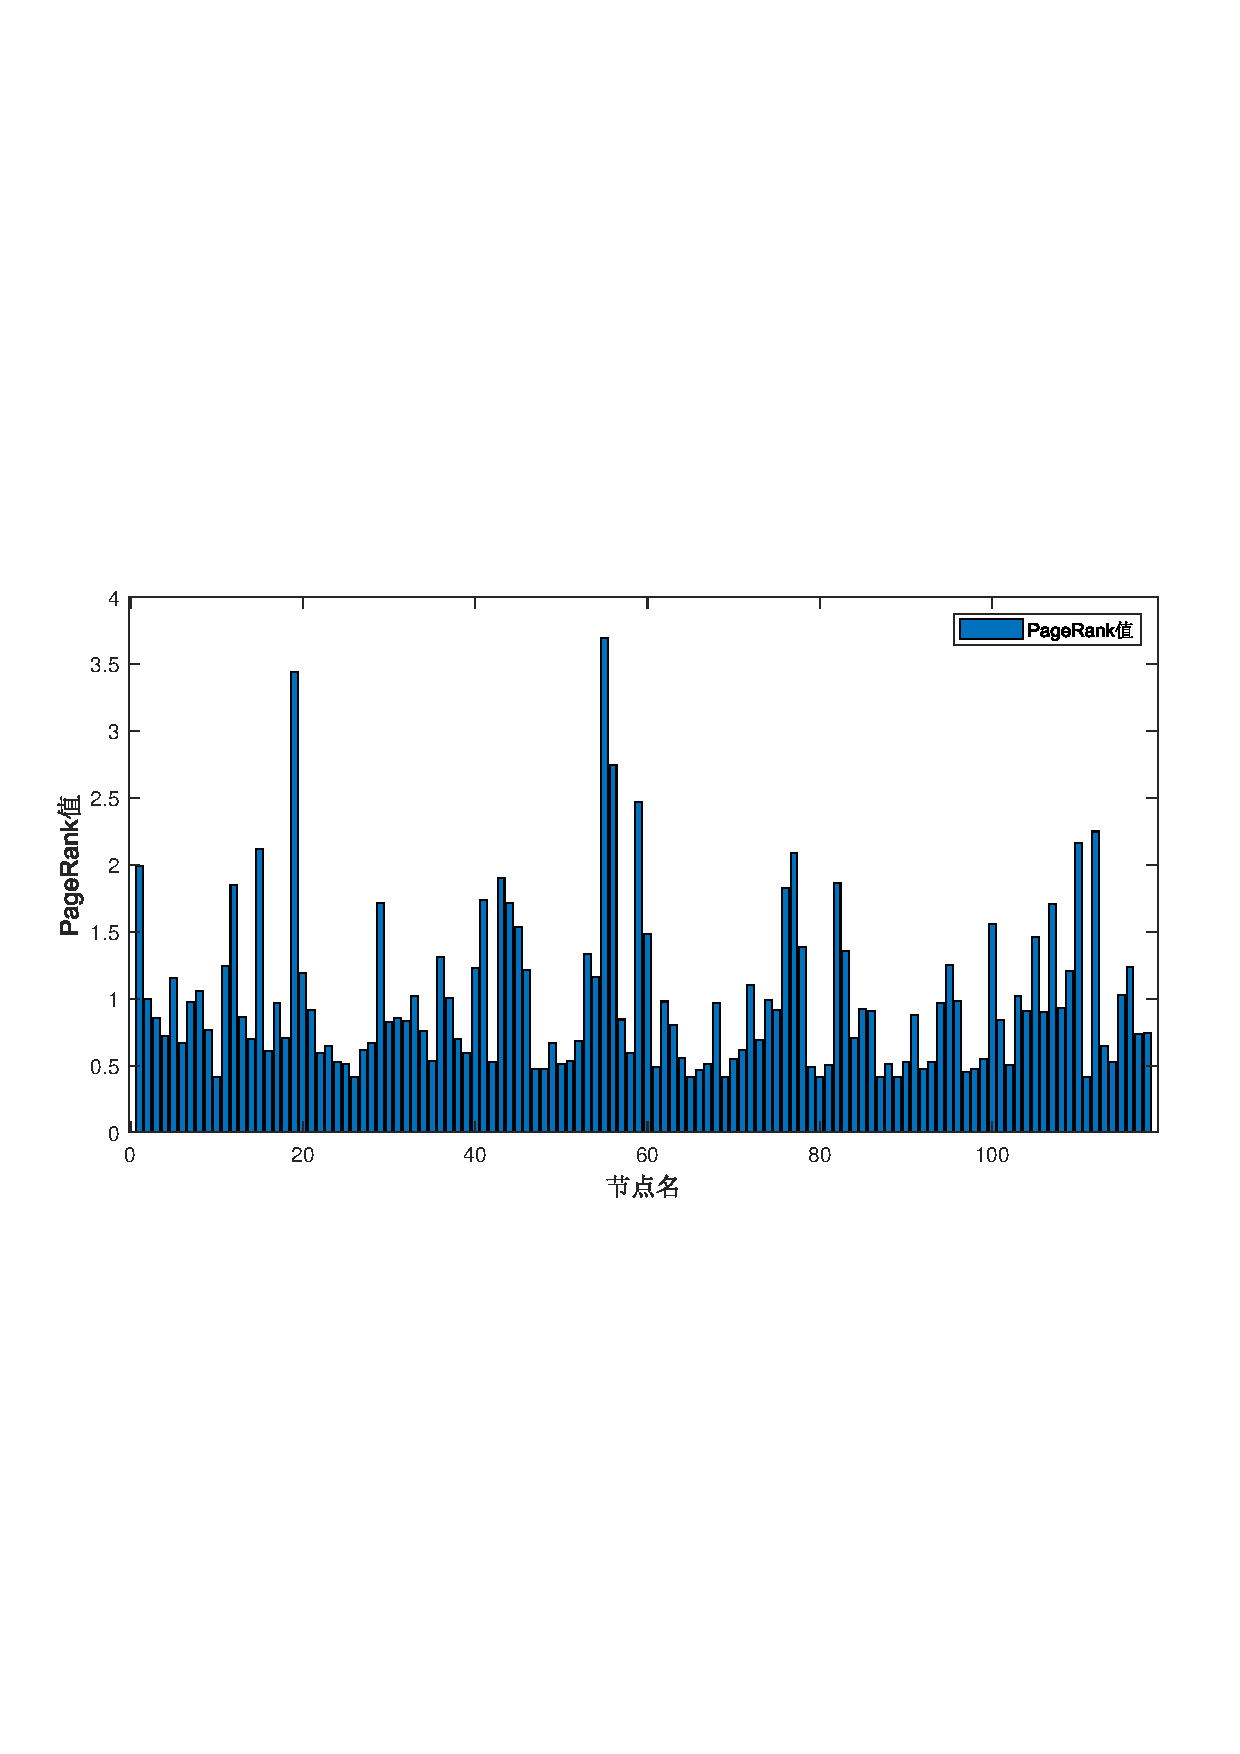
\includegraphics[width=14cm,height=7cm]{PageRank118.pdf}
%     \caption{$IEEE118$节点PageRank值计算结果图}
%     \label{fig:pagerank118}
% \end{figure}

% 从图\ref{fig:electricDu118}、\ref{fig:nodeBetween118}和\ref{fig:pagerank118}可以看出,电气度指标值较高的节点名有9、8、49、5、30、89等,这些节点在电网结构中的邻接节点较多,
% 所连支路承担的潮流值较大;电气介数指标值较高的节点名有100、65、80、49、103等,表明电气介数值较大节点在结构和能量传输方面的重要程度高;PageRank指标值较高的节点名有1、55、19、56、59等,
% 这些节点的入链数目多,在潮流累计分布中比重较大。因此,在电网结构中的重要程度高。

% 下面为电气度、电气介数、$PageRank$值按照重要程度的节点号排名,取移除比例为$30\%$的节点数量。如表\ref{tab:rank118}所示。
% \begin{table}[H]
%     \centering
%     \caption{电气度、电气介数、$PageRank$值节点号排名}
%     \label{tab:rank118}
%       \begin{tabular}{C{3cm}C{3cm}C{3cm}C{4cm}}
%         \toprule
%         节点排名  & 电气度节点名   & 电气介数节点名     & PageRank值节点名\\
%         \midrule
%         1       & 9              & 100                & 1 \\
%         2       & 8              & 65                 & 55 \\
%         3       & 49             & 80                 & 19 \\
%         4       & 5              & 49                 & 56 \\
%         5       & 30             & 103                 & 59 \\
%         6       & 89             & 94                 & 112 \\
%         7       & 69             & 8                 & 110 \\
%         8       & 37             & 5                 & 15 \\
%         9       & 38             & 77                 & 77 \\
%         10      & 65             & 25                 & 43 \\
%         11      & 17               & 61                & 82 \\
%         12      & 92               & 68                 & 12 \\
%         13      & 80               & 12                 & 76 \\
%         14      & 10                 & 54                 & 41 \\
%         15      & 68                 & 26                 & 44 \\
%         16      & 66                 & 59                 & 29 \\
%         17      & 25                 & 10                 & 107 \\
%         18      & 64                 & 38                 & 100 \\
%         19      & 77                 & 89                 & 45 \\
%         20      & 59                 & 9                 & 60 \\
%         21      & 100                & 30                 & 105 \\
%         22      & 63                 & 11                 & 78 \\
%         23      & 23                 & 69                 & 83 \\
%         24      & 26                 & 37                 & 53 \\
%         25      & 103                & 45                 & 36 \\
%         26      & 75                 & 110                 & 95 \\
%         27      & 85                 & 111                 & 11 \\
%         28      & 11                 & 17                 & 116 \\
%         29      & 61                 & 60                 & 40 \\
%         30      & 27                 & 75                 & 46 \\
%         31      & 94                 & 96                 & 109 \\
%         32      & 116                 & 64                 & 20 \\
%         33      & 110                 & 78                 & 54 \\
%         34      & 90                 & 23                 & 5 \\
%         35      & 4                 & 82                 & 72 \\
%         36      & 12                 & 46                 & 8 \\
%         37      & 60                & 88                 & 115 \\
%         38      & 70                 & 56                 & 33 \\
%         39      & 42                & 81                 & 103 \\
%         \bottomrule
%       \end{tabular}
% \end{table}

% 下面为四种攻击策略下的仿真结果,如图\ref{fig:chap5:4Efficiency118}、\ref{fig:chap5:Efficiency118}所示。
% \begin{figure}[H] % use float package if you want it here
%   \centering
%   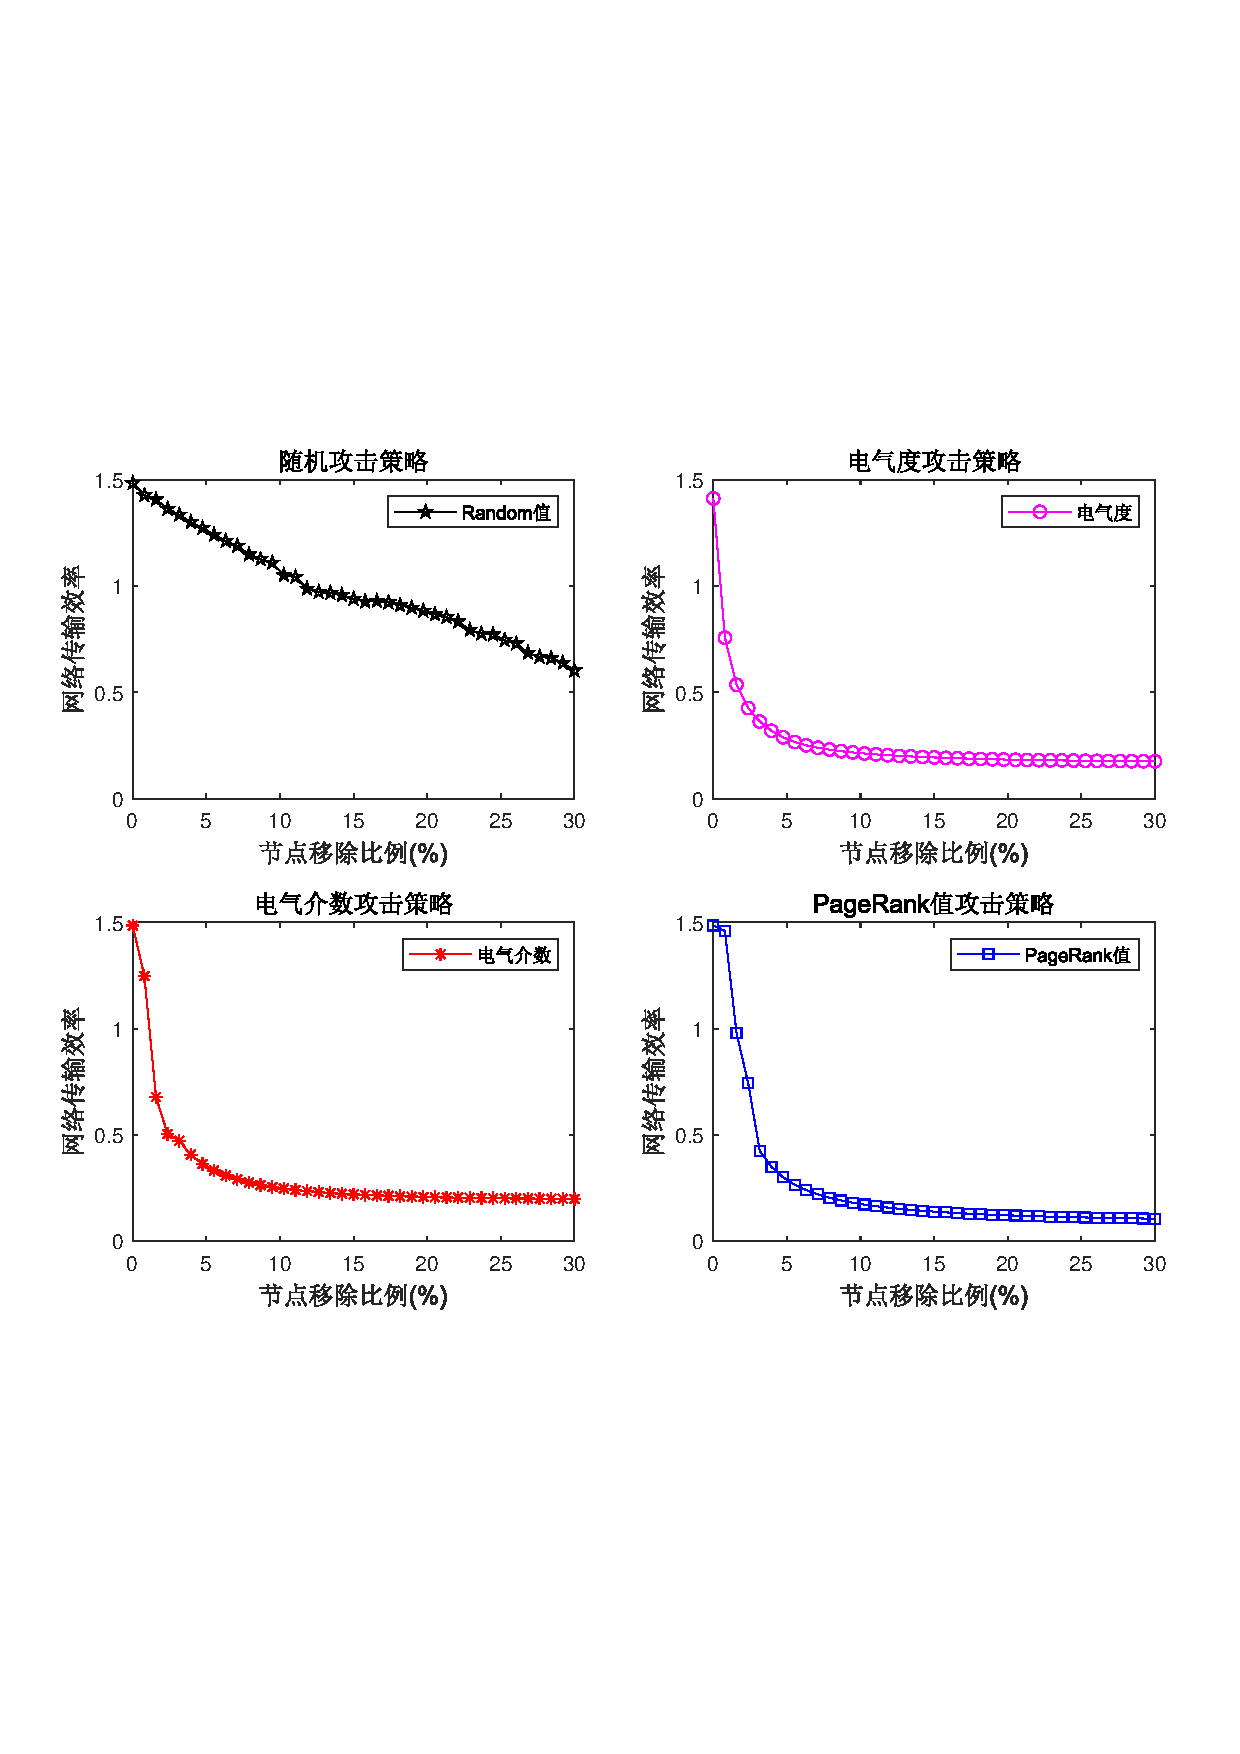
\includegraphics[width=13.4cm,height=9.6cm]{4Efficiency118.pdf}
%   \caption{四种攻击策略下电网平均传输效率趋势图}
%   \label{fig:chap5:4Efficiency118}
% \end{figure}
% \begin{figure}[H] % use float package if you want it here
%   \centering
%   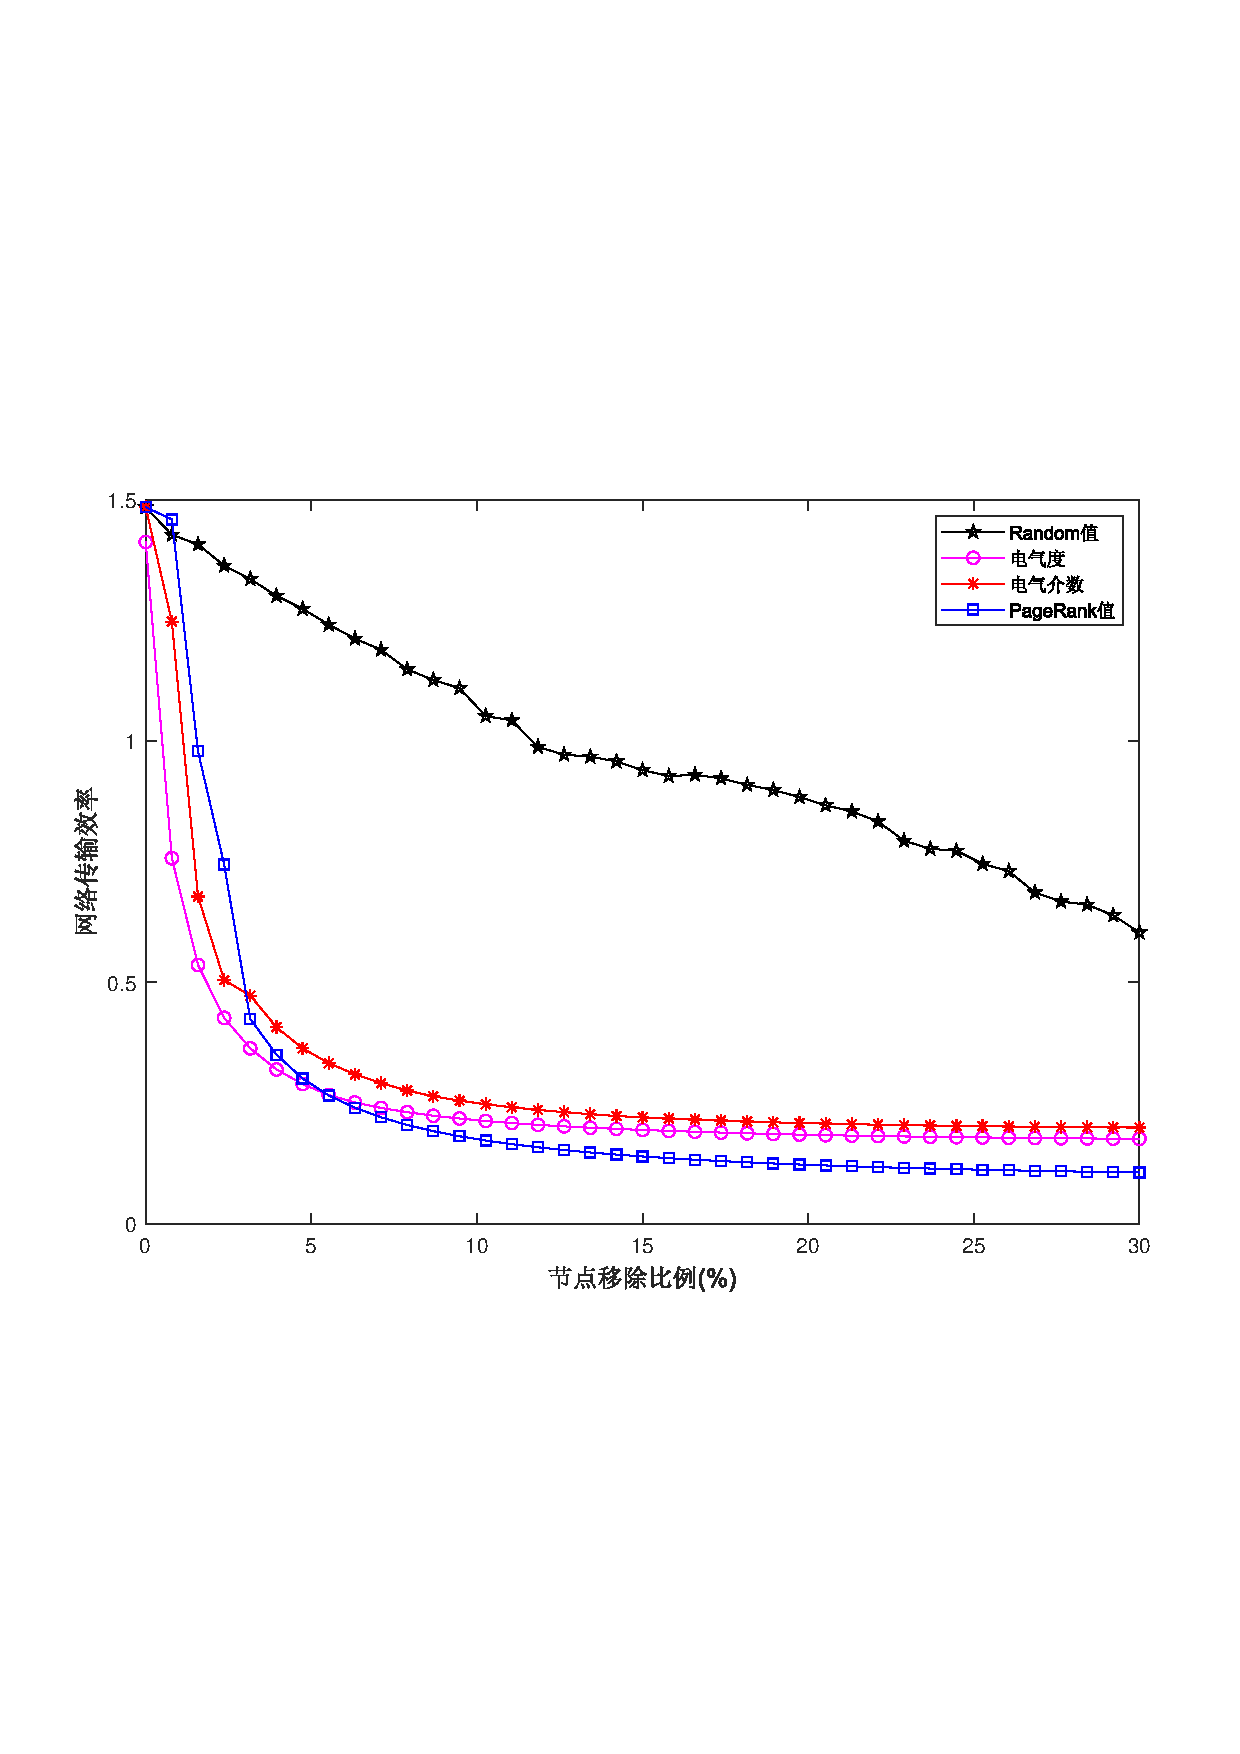
\includegraphics[width=13.4cm,height=9.1cm]{Efficiency118.pdf}
%   \caption{四种电网攻击策略结果对比图}
%   \label{fig:chap5:Efficiency118}
% \end{figure}

% 从图\ref{fig:chap5:4Efficiency118}、\ref{fig:chap5:Efficiency118}的实验结果可以看出:

% $(1)$在随机攻击策略下,网络传输效率值下降较为平缓,在节点移除比例至$30\%$时,电网的传输效率约为原来传输效率的$40\%$。而与其他三种攻击策略相比,
% 电气度、电气介数和$PageRank$值攻击策略对于电网传输效率的破坏性更高,在移除比例约为$10\%$时,电网平均传输效率已分别降至原来的$14.9\%$、$17.6\%$和$12.8\%$。因此,本文基于复杂网络
% 理论得到的脆弱性指标可以科学合理地描述系统各节点在电网中的重要程度,并可进一步衡量各节点在电网中的脆弱性。

% $(2)$随机攻击策略对于电网的连通性影响较小,而蓄意攻击将会对网络连通性及传输效率影响较大,说明电网对于随机攻击具有很好的鲁棒性,进一步证实了电网的无标度性。

% $(3)$对比三种蓄意攻击策略,从图\ref{fig:chap5:Efficiency118}得到,在节点移除前期,电气度攻击对于电网平均传输效率下降趋势最为明显,其原因在于,电气度是基于节点度进行定义的,电气度
% 指标更多的是专注于电网拓扑结构的重要性。在电气度的攻击策略下,节点的移除时意味着最大程度切断其他节点与所移除节点的联系,这将极大地破坏电网的拓扑结构,进而影响电网传输性能。可以证实,
% 电网拓扑结构的稳定性是电力系统正常运行的重要保证和前提条件,其节点的分布和联系是影响电网脆弱性的重要因素。在节点移除的后期,电气度、电气介数和$PageRank$值攻击策略对电网传输效率值分别
% 下降为$11.71\%$、$13.26\%$、$7.06\%$,在后期的移除过程中,$PageRank$值攻击策略的破坏性更高,原因在于,$PageRank$值指标关注的是潮流流向对于电网结构的重要性,指向节点的潮流数越多意味着
% 此节点的重要性越高,按照此攻击策略进行移除,将会导致发电节点所传输的功率所供给的节点越来越少,传输效率下降,直至无法进行功率传输。

% 综上分析,电气度、电气介数和$PageRank$的攻击策略相较于随机攻击策略的破坏性较大,指标值较大的节点在遭到破坏时,电网结构受影响程度较大,从而验证了这三种指标可作为脆弱性指标的合理性。
% 通过三种蓄意攻击策略的对比,可得到电气度专注于电网结构拓扑的重要性,PageRank值则侧重于节点入链数的重要性,而电气介数综合考虑节点支路和支路潮流对电网结构的影响程度,其攻击策略对电网的破坏性
% 较为均衡。


\section{电网脆弱性评估分析}
\label{sec:singleAssessment}

本文基于$IEEE39$标准电网算例对电网脆弱性的研究工作,分别从结构和状态两个方面研究系统脆弱性,分析各系统节点对电网拓扑结构的影响程度,以及各节点对于电网故障及扰动的能力,最后将结构与状态
这两方面进行融合,综合评价系统的脆弱性,识别出电力系统的脆弱环节。

\subsection{电网结构脆弱性实验分析}
\label{sec:singleAnalysis_fabric}
本文选择的电网仿真模型为新英格兰测试系统数据——$IEEE39$,该系统由10个发电节点、29个负荷节点和46条支路组成。该系统的基准电压为345$KV$,基准功率为100$MVA$。
负荷节点序号为1-29;发电节点序号为30—39;31号节点为平衡节点。具体模型数据见附录A。

针对$IEEE39$标准算例系统的节点连接情况,可以得到如下的电网结构示意图。
\begin{figure}[H] % use float package if you want it here
  \centering
  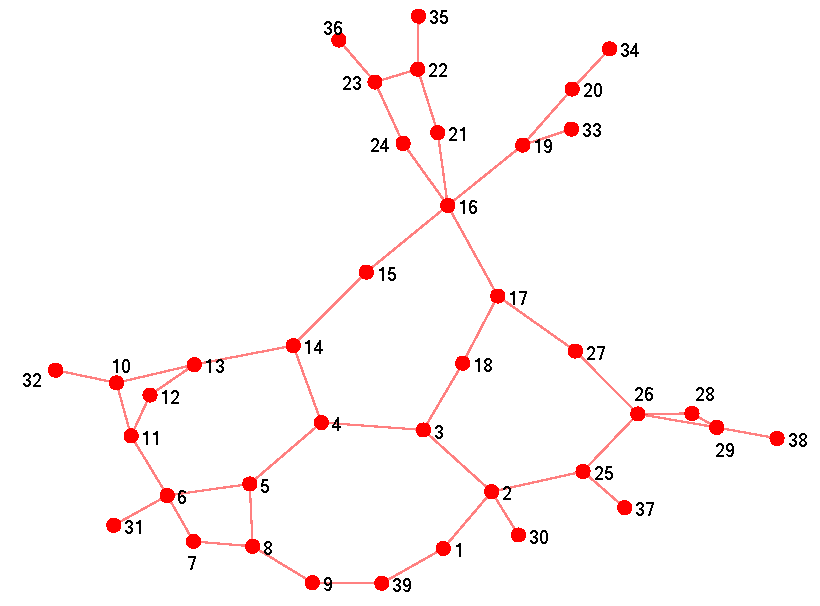
\includegraphics[height=7.5cm]{fabric_39.pdf}
  \caption{$IEEE39$系统拓扑示意图}
  \label{fig:fabric_39}
\end{figure}

\begin{figure}[H] % use float package if you want it here
  \centering
  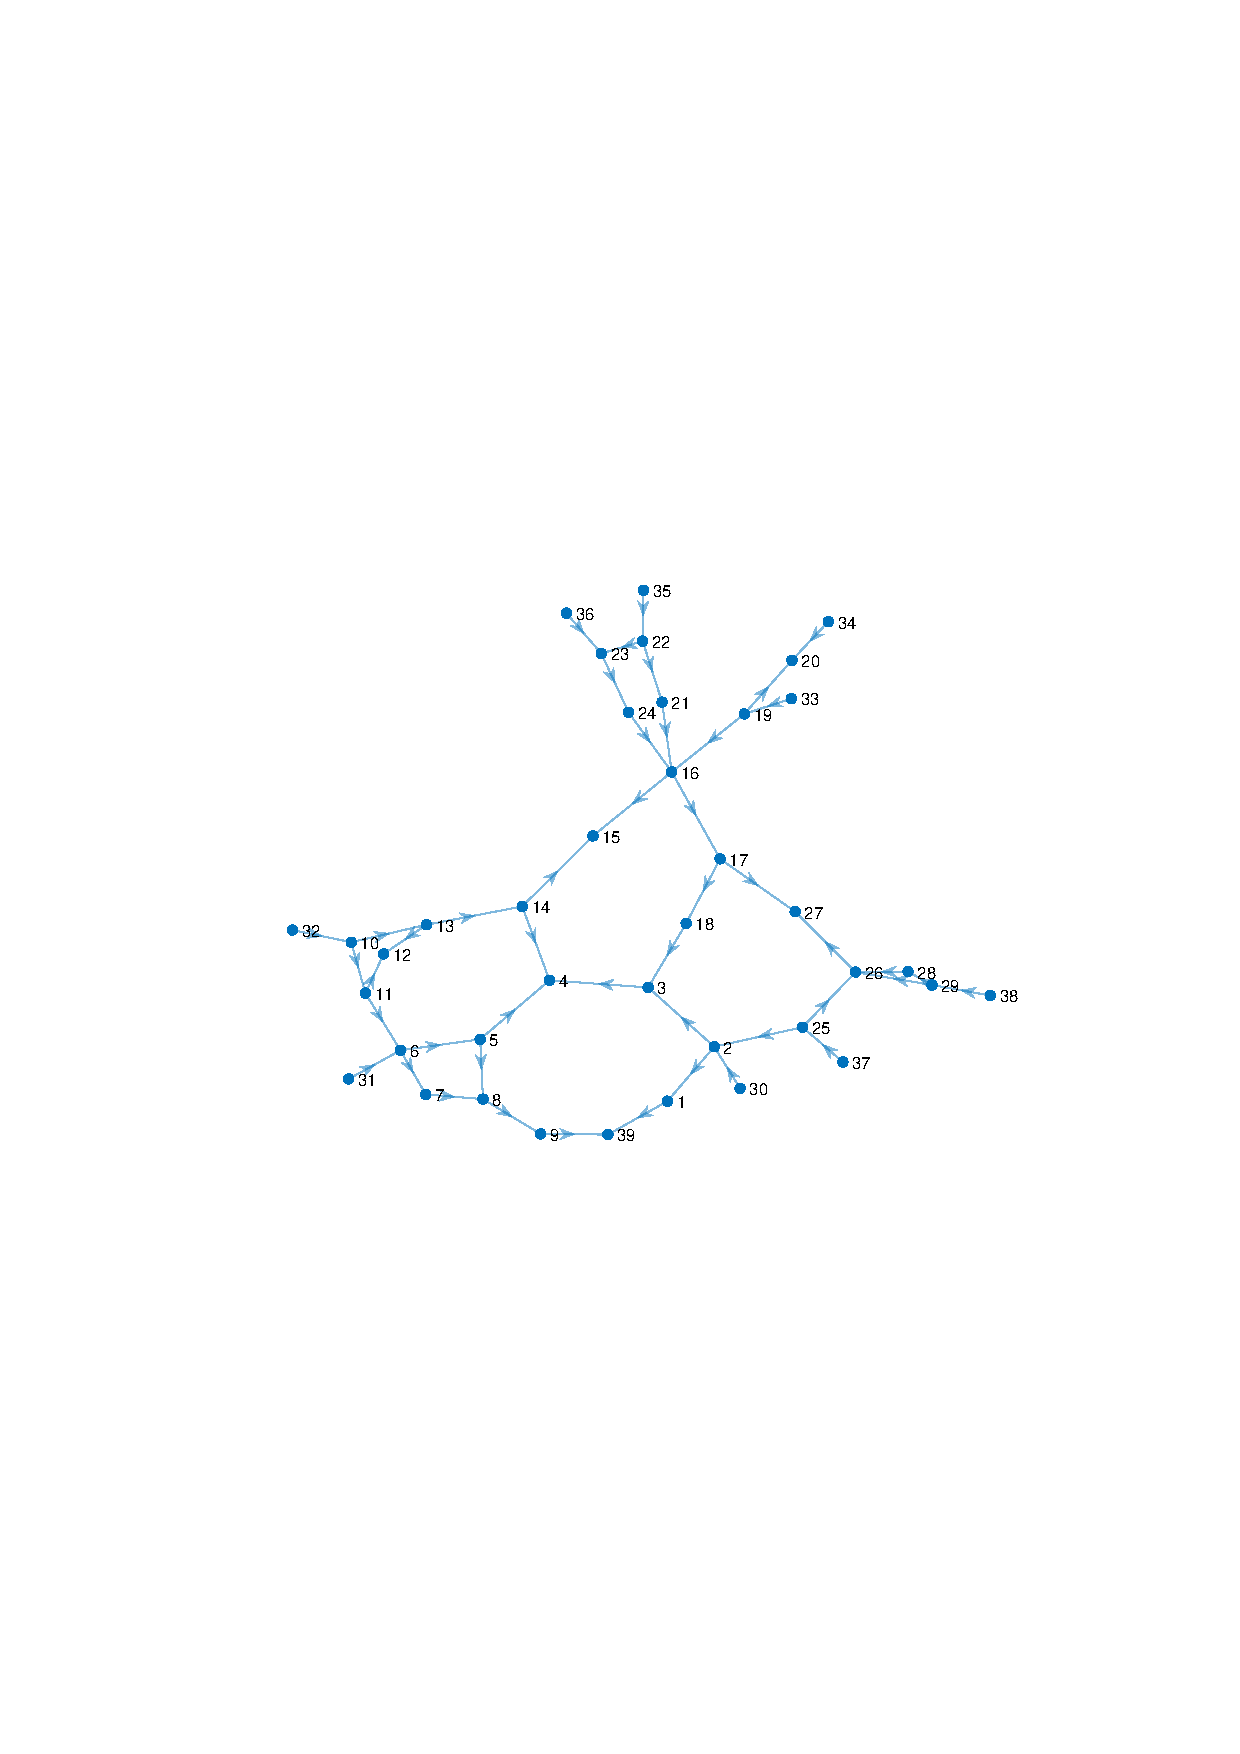
\includegraphics[height=8cm]{PageRank_39.pdf}
  \caption{$IEEE39$系统潮流有向图}
  \label{fig:PageRank_39}
\end{figure}


电气度、电气介数和$PageRank$值是基于复杂网络理论从不同的角度提出的结构脆弱性评价指标,为了不改变指标数据的原始分布,充分反映的是系统各节点在结构中的重要程度,对于结构脆弱性指标采用离散标准化的
归一化方法,得到各结构脆弱性指标数据后,采用改进的熵权法对电气度、电气介数和$PageRank$值这三个指标进行权重分配,得到权重向量$W_1 = \left[w_{1}\ w_{2}\ w_{3}\right]=[0.33\ 0.41\ 0.26]$,
并融合得到结构综合脆弱性指标。如表~\ref{tab:chap5:Index_frabric39}~和图~\ref{fig:stric_3index}~所示。
\begin{table}[H]
  \centering
  \caption{$IEEE39$系统结构脆弱性指标}
  \label{tab:chap5:Index_frabric39}
  \begin{tabular}{C{1.5cm}C{2.05cm}C{2.5cm}C{2.85cm}C{3.5cm}}
  \toprule
  \textbf{节点序号} & \textbf{电气度指标} & \textbf{电气介数指标} & \textbf{PageRank值指标} & \textbf{结构综合脆弱性指标} \\
  \midrule
  1 & 0.086924952 & 0.230348929 & 0.131020681 & 0.157193672 \\ 
  2 & 0.507756514 & 0.713870587 & 0.298554703 & 0.537870813 \\ 
  3 & 0.212417624 & 0.711647114 & 0.639183338 & 0.528060801 \\ 
  4 & 0.260485416 & 0.572099497 & 1           & 0.580520981 \\ 
  5 & 0.518219694 & 0.226085642 & 0.209128679 & 0.318081069 \\ 
  6 & 1           & 0.503485706 & 0.314075081 & 0.61808866 \\
  7 & 0.309635969 & 0.277191576 & 0.179009284 & 0.26237083 \\ 
  8 & 0.319050739 & 0.608998063 & 0.462906823 & 0.475331724 \\ 
  9 & 0.047102245 & 0.451887203 & 0.514658016 & 0.334628578 \\ 
  10 & 0.644344321 & 0.690312667 & 0.121158521 & 0.527163035 \\ 
  11 & 0.321857272 & 0.424945152 & 0.114064772 & 0.310097253 \\ 
  12 & 0           & 0           & 0.052371565 & 0.013616607 \\
  13 & 0.313506292 & 0.252871293 & 0.110080368 & 0.235755202 \\ 
  14 & 0.294699744 & 0.244978418 & 0.187549614 & 0.246454967 \\ 
  15 & 0.150832887 & 0.380901879 & 0.508650374 & 0.33819372 \\ 
  16 & 0.702443253 & 1           & 0.782654015 & 0.845296317 \\ 
  17 & 0.203569872 & 0.207053465 & 0.332121968 & 0.23842169 \\ 
  18 & 0.08070881  & 0.182479179 & 0.32250596  & 0.18530192 \\ 
  19 & 0.613414417 & 0.676656584 & 0.121158521 & 0.511357172 \\ 
  20 & 0.316762885 & 0.692736421 & 0.183458526 & 0.436252901 \\ 
  21 & 0.445971669 & 0.664135765 & 0.204129549 & 0.472539997 \\ 
  22 & 0.653758374 & 0.687089744 & 0.121158521 & 0.528948274 \\ 
  23 & 0.462785664 & 0.693184789 & 0.141174112 & 0.473630302 \\ 
  24 & 0.194520487 & 0.383108926 & 0.241158154 & 0.28396754 \\ 
  25 & 0.408317466 & 0.66937866  & 0.121158521 & 0.44069123 \\ 
  26 & 0.303558847 & 0.402464484 & 0.370358706 & 0.361478121 \\ 
  27 & 0.119219078 & 0.33135194  & 0.516940852 & 0.309601212 \\ 
  28 & 0.210788875 & 0.25769646  & 0.144614587 & 0.21281567 \\ 
  29 & 0.670307453 & 0.683970816 & 0.121158521 & 0.53313071 \\ 
  30 & 0.105556919 & 0.510686205 & 0           & 0.244215127 \\ 
  31 & 0.306737872 & 0.026491918 & 0           & 0.112085184 \\ 
  32 & 0.29880342  & 0.690312667 & 0           & 0.381633322 \\ 
  33 & 0.283977411 & 0.68455485  & 0           & 0.374380034 \\ 
  34 & 0.22519754  & 0.665173423 & 0           & 0.347036292 \\ 
  35 & 0.302835147 & 0.690312667 & 0           & 0.382963792 \\ 
  36 & 0.246277315 & 0.676175494 & 0           & 0.358503467 \\ 
  37 & 0.237532647 & 0.673137612 & 0           & 0.354372194 \\ 
  38 & 0.387392146 & 0.690559802 & 0           & 0.410968927 \\ 
  39 & 0.015510059 & 0.695379301 & 0.791086603 & 0.49590635 \\ 
  \bottomrule
  \end{tabular}
\end{table}

\begin{figure}[H] % use float package if you want it here
  \centering
  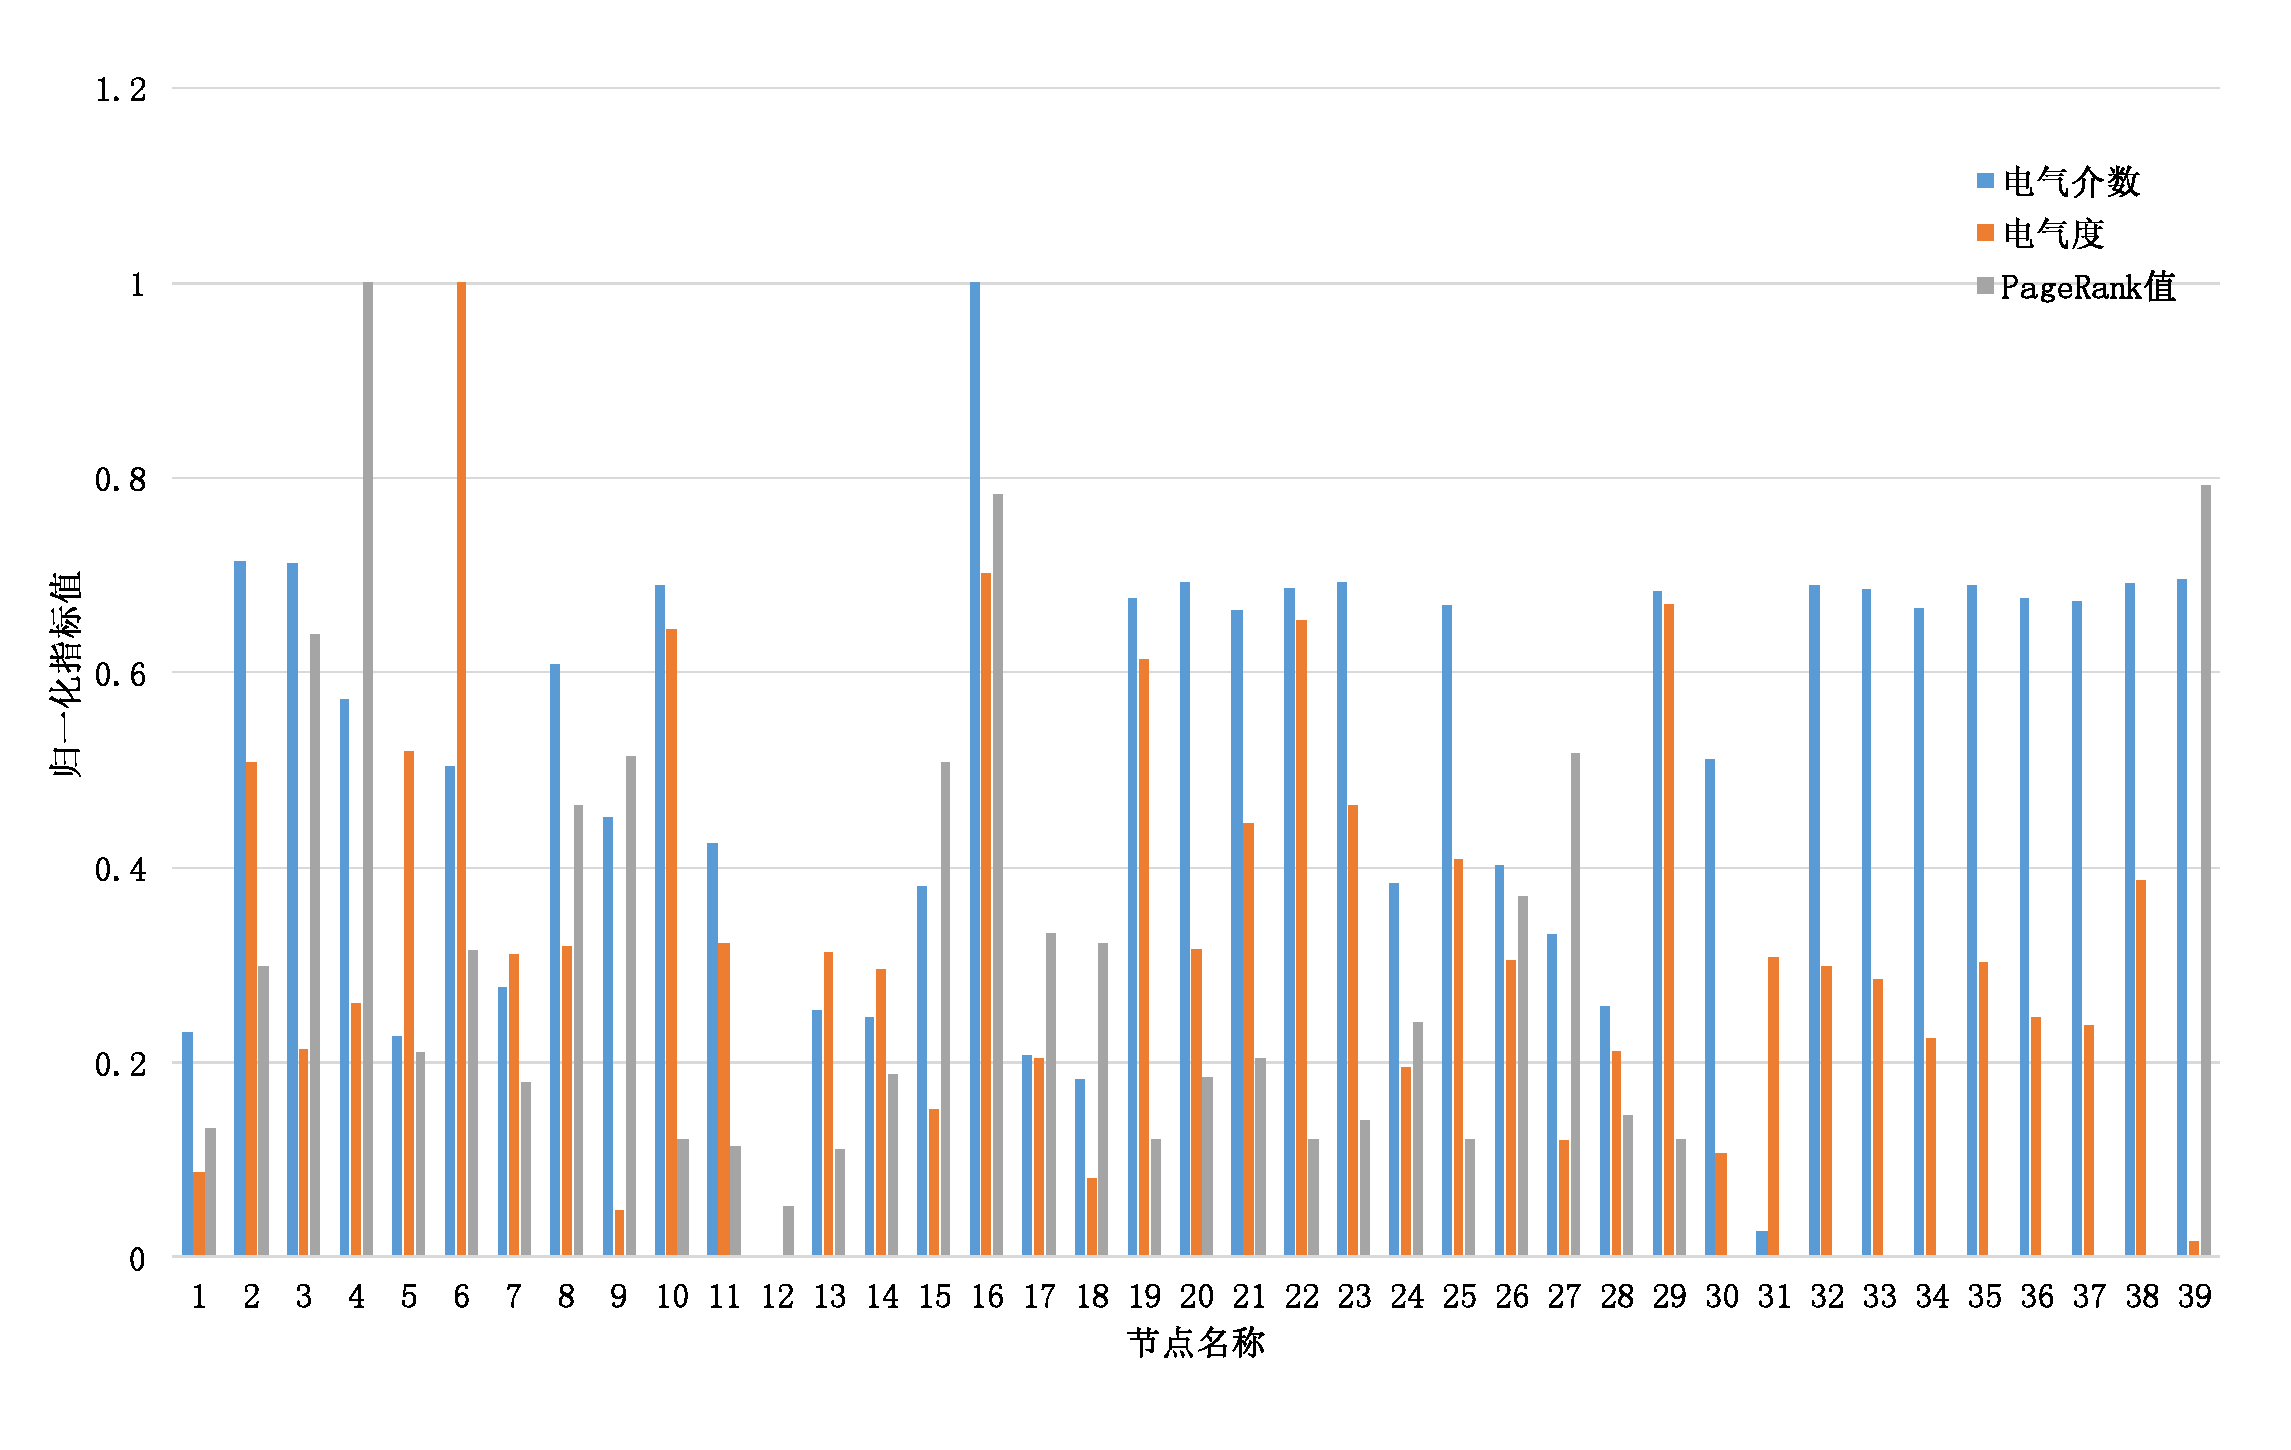
\includegraphics[width=14cm,height=8.1cm]{stric_3index.pdf}
  \caption{$IEEE39$节点各结构脆弱性指标}
  \label{fig:stric_3index}
\end{figure}

在$IEEE39$系统中,电气度指标值最大的为节点6,最小的为节点12;电气介数指标值最大的为节点16,最小的为节点12;PageRank值最大的为节点4,最小的为发电节点30、31、32、33、34、35、36、37、38。
在基于$PageRank$的$IEEE39$拓扑模型中,发电节点30—38无入链数,并且其出链数均为1,所以其$PageRank$值相同且最小。对于节点12,其电气度和电气介数指标值均最小,从$IEEE39$电网结构
拓扑图中可以看出节点12与节点11和节点13连接,节点度较小,除此之外,根据附录A中$IEEE39$系统数据,其功率容量较小,并且节点11和节点13均为联络节点(无功率容量),这导致节点12所连接支路的
视在功率较小,从而计算得到的电气度指标值较小。节点电气介数是综合结构和潮流能量进行定义的,该指标值与支路和节点的有功功率容量正相关,因此,在$IEEE39$系统中,节点12的电气介数值最小。
节点6和16在节点度和支路潮流值上,较其他节点都比较大,因此,根据电气度和电气介数的计算方法,其指标数值最大。

根据权重向量计算得到的系统结构综合脆弱性指标结果如图\ref{fig:stric_39}所示。
\begin{figure}[H] % use float package if you want it here
  \centering
  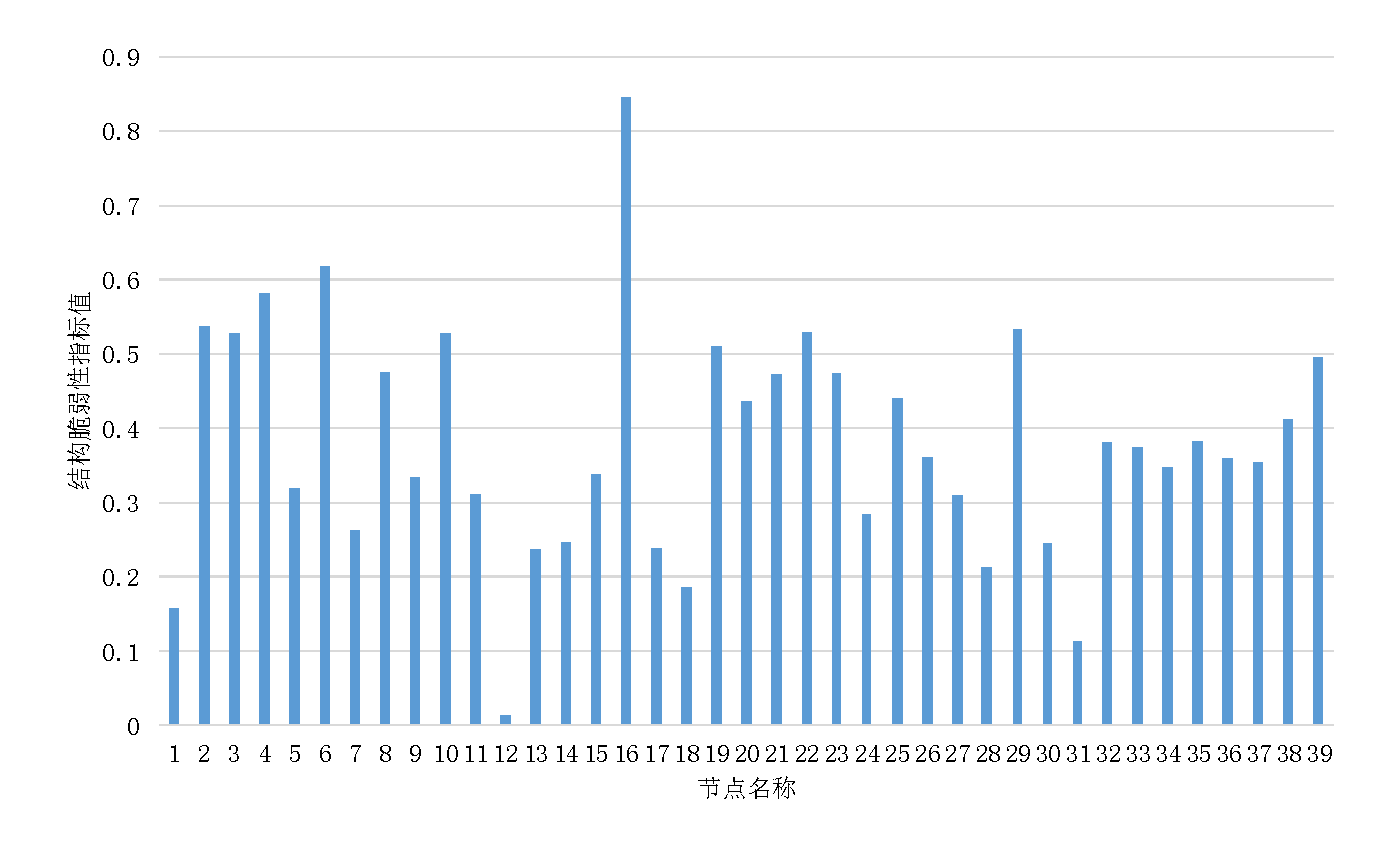
\includegraphics[width=14cm,height=8.64cm]{stric_39.pdf}
  \caption{$IEEE39$节点结构综合脆弱性指标}
  \label{fig:stric_39}
\end{figure}

从图\ref{fig:stric_39}可知,系统结构综合脆弱性最高的节点是16。从表\ref{tab:chap5:Index_frabric39}其在电气度、电气介数和$PageRank$值中的指标数值分别为0.7、1和0.78,从这
三个指标角度考虑来看,节点16在此系统结构的重要程度较高。从结构示意图不难看出,节点16位于系统结构的中心位置,与其连接的有15、17、19、21和24节点,综合图\ref{fig:PageRank_39}来看,
节点16的入链数3条,出链数2条,较其他节点而言,节点16所连支路承担着较多的能量传输,假设节点16发生故障,$IEEE39$电网系统会随即裂解成三个子网络,从而影响电网网运行。节点2、4、6、
10、29的重要性也比较高,从节点位置可以看出,这些节点大都连接发电节点,如节点30、31、32、38,承担着将发电节点产生的能量传送至各负荷节点,支路潮流值较大。因此,这些节点不论从节点
连接情况和潮流分布情况而言对于系统结构起到重要作用,所以这些节点的结构综合脆弱程度高。另一方面,节点12、31、1、18、28的结构综合脆弱性指标值较小,所连节点一般为联络节点或容量较小的负荷节点,
其节点节点容量潮流累计和支路潮流值较小,假设这些节点发生故障,并不会对系统结构的完整性造成较大的影响,因此,这些节点的结构位置在系统中的作用较小,所连支路对于电能的传输能力也较小,
故其结构综合脆弱程度低。

通过上述结构脆弱性实验分析可得出,在结构脆弱性分析结果方面,节点的传输能力越大,所处位置的重要性越高,即节点所连支路越多,节点的结构脆弱性越强。

\subsection{电网状态脆弱性实验分析}
\label{sec:singleAnalysis_status}
在状态脆弱性指标集中,本文通过模拟实际电网负荷变化,通过潮流计算得到电压稳定裕度指标值,采用第三章所建立的正态分布负荷模型中,如式\ref{equ:chap3:probability}所示,其中均值$\mu$设置为
对应负荷节点的额定功率,标准差$\sigma$为负荷节点额定功率的$0.2$倍,所以电网负荷模型负荷功率95.45$\%$分布在额定功率的0.8到1,2倍之间,并通过蒙特卡洛模拟实验进行仿真,仿真次数为10000,
以式\ref{equ:chap3:SV}进行计算,取平均值作为最终结果;在功率裕度指标计算中,式\ref{equ:chap3:SC}中,最大负荷功率依据式\ref{equ:chap3:probability1}通过连续潮流计算得到,其中$Q_{target}$
设置为1.5倍的额定功率;在电网损耗灵敏度指标计算中,每个负荷节点在额定负荷$\pm 10 \%$范围内取100个计算点进行潮流计算,所以步长设置为负荷节点0.002倍的额定功率。
根据系统节点各状态脆弱性指标值结果,基于最大离差化法得到权重向量$W_2 = \left[w_{1}\ w_{2}\ w_{3}\right]=[0.29\ 0.34\ 0.37]$并融合得到结构综合脆弱性指标。
如表\ref{tab:chap5:Index2_frabric39}所示。由于状态脆弱性指标集均基于负荷模型进行仿真实验,故在状态脆弱性研究时仅针对负荷节点进行分析。

\begin{table}[H]
  \centering
  \caption{$IEEE39$系统状态脆弱性指标}
  \label{tab:chap5:Index2_frabric39}
  \begin{tabular}{C{1.5cm}C{2.5cm}C{2.5cm}C{2.75cm}C{2.75cm}}
  \toprule
  \textbf{节点序号} & \textbf{电压裕度指标} & \textbf{功率稳定裕度指标} & \textbf{电网损耗灵敏度指标} & \textbf{状态综合脆弱性指标} \\
  \midrule
  1 & 0           & 0.856470588 & 0.333864456 & 0.414729849 \\
  2 & 0.627763605 & 0           & 0           & 0.182051445 \\ 
  3 & 0.868532753 & 0.526470588 & 0.173992035 & 0.495251552 \\ 
  4 & 0.681365198 & 0.264705882 & 0.175148734 & 0.352400939 \\
  5 & 0.548173985 & 0           & 0           & 0.158970456 \\ 
  6 & 0.513990896 & 0           & 0           & 0.14905736 \\ 
  7 & 0.493134944 & 0.656176471 & 0.187816277 & 0.435601156 \\ 
  8 & 0.440628844 & 0.232352941 & 0.243415763 & 0.296846197 \\ 
  9 & 0.234327507 & 0.990441176 & 0.318257774 & 0.522460353 \\ 
  10 & 0.615287695 & 0          & 0           & 0.178433432 \\ 
  11 & 0.585145902 & 0          & 0           & 0.169692312 \\
  12 & 0.52049683  & 0.987455882 & 0.113091151 & 0.528522806 \\ 
  13 & 0.64839947  & 0           & 0           & 0.188035846 \\ 
  14 & 0.742688646 & 0           & 0           & 0.215379707 \\
  15 & 0.643616556 & 0.529411765 & 0.04447175  & 0.383103349 \\ 
  16 & 0.69500044  & 0.516176471 & 0.106956156 & 0.416623905 \\ 
  17 & 0.831020315 & 0           & 0           & 0.240995891 \\ 
  18 & 0.885074662 & 0.767647059 & 0.0783821   & 0.546673029 \\ 
  19 & 1           & 0           & 0           & 0.29 \\ 
  20 & 0.221686653 & 0           & 0.413774827 & 0.217385815 \\ 
  21 & 0.473735759 & 0.597058824 & 0.256847857 & 0.435417077 \\ 
  22 & 0.411534686 & 0           & 0           & 0.119345059 \\
  23 & 0.345775724 & 0.636029412 & 0.509079018 & 0.504884197 \\ 
  24 & 0.622365665 & 0.546176471 & 0.111699933 & 0.407515018 \\
  25 & 0.460615009 & 0.670588235 & 0.776181665 & 0.648765569 \\ 
  26 & 0.748966045 & 0.795588235 & 0.443079199 & 0.651639457 \\ 
  27 & 0.657596651 & 0.586764706 & 0.150193042 & 0.445774454 \\ 
  28 & 0.490373345 & 0.697058824 & 0.753896625 & 0.658150021 \\ 
  29 & 0.588829917 & 0.583088235 & 1           & 0.739010676 \\ 
  \bottomrule
  \end{tabular}
\end{table}

\begin{figure}[H] % use float package if you want it here
  \centering
  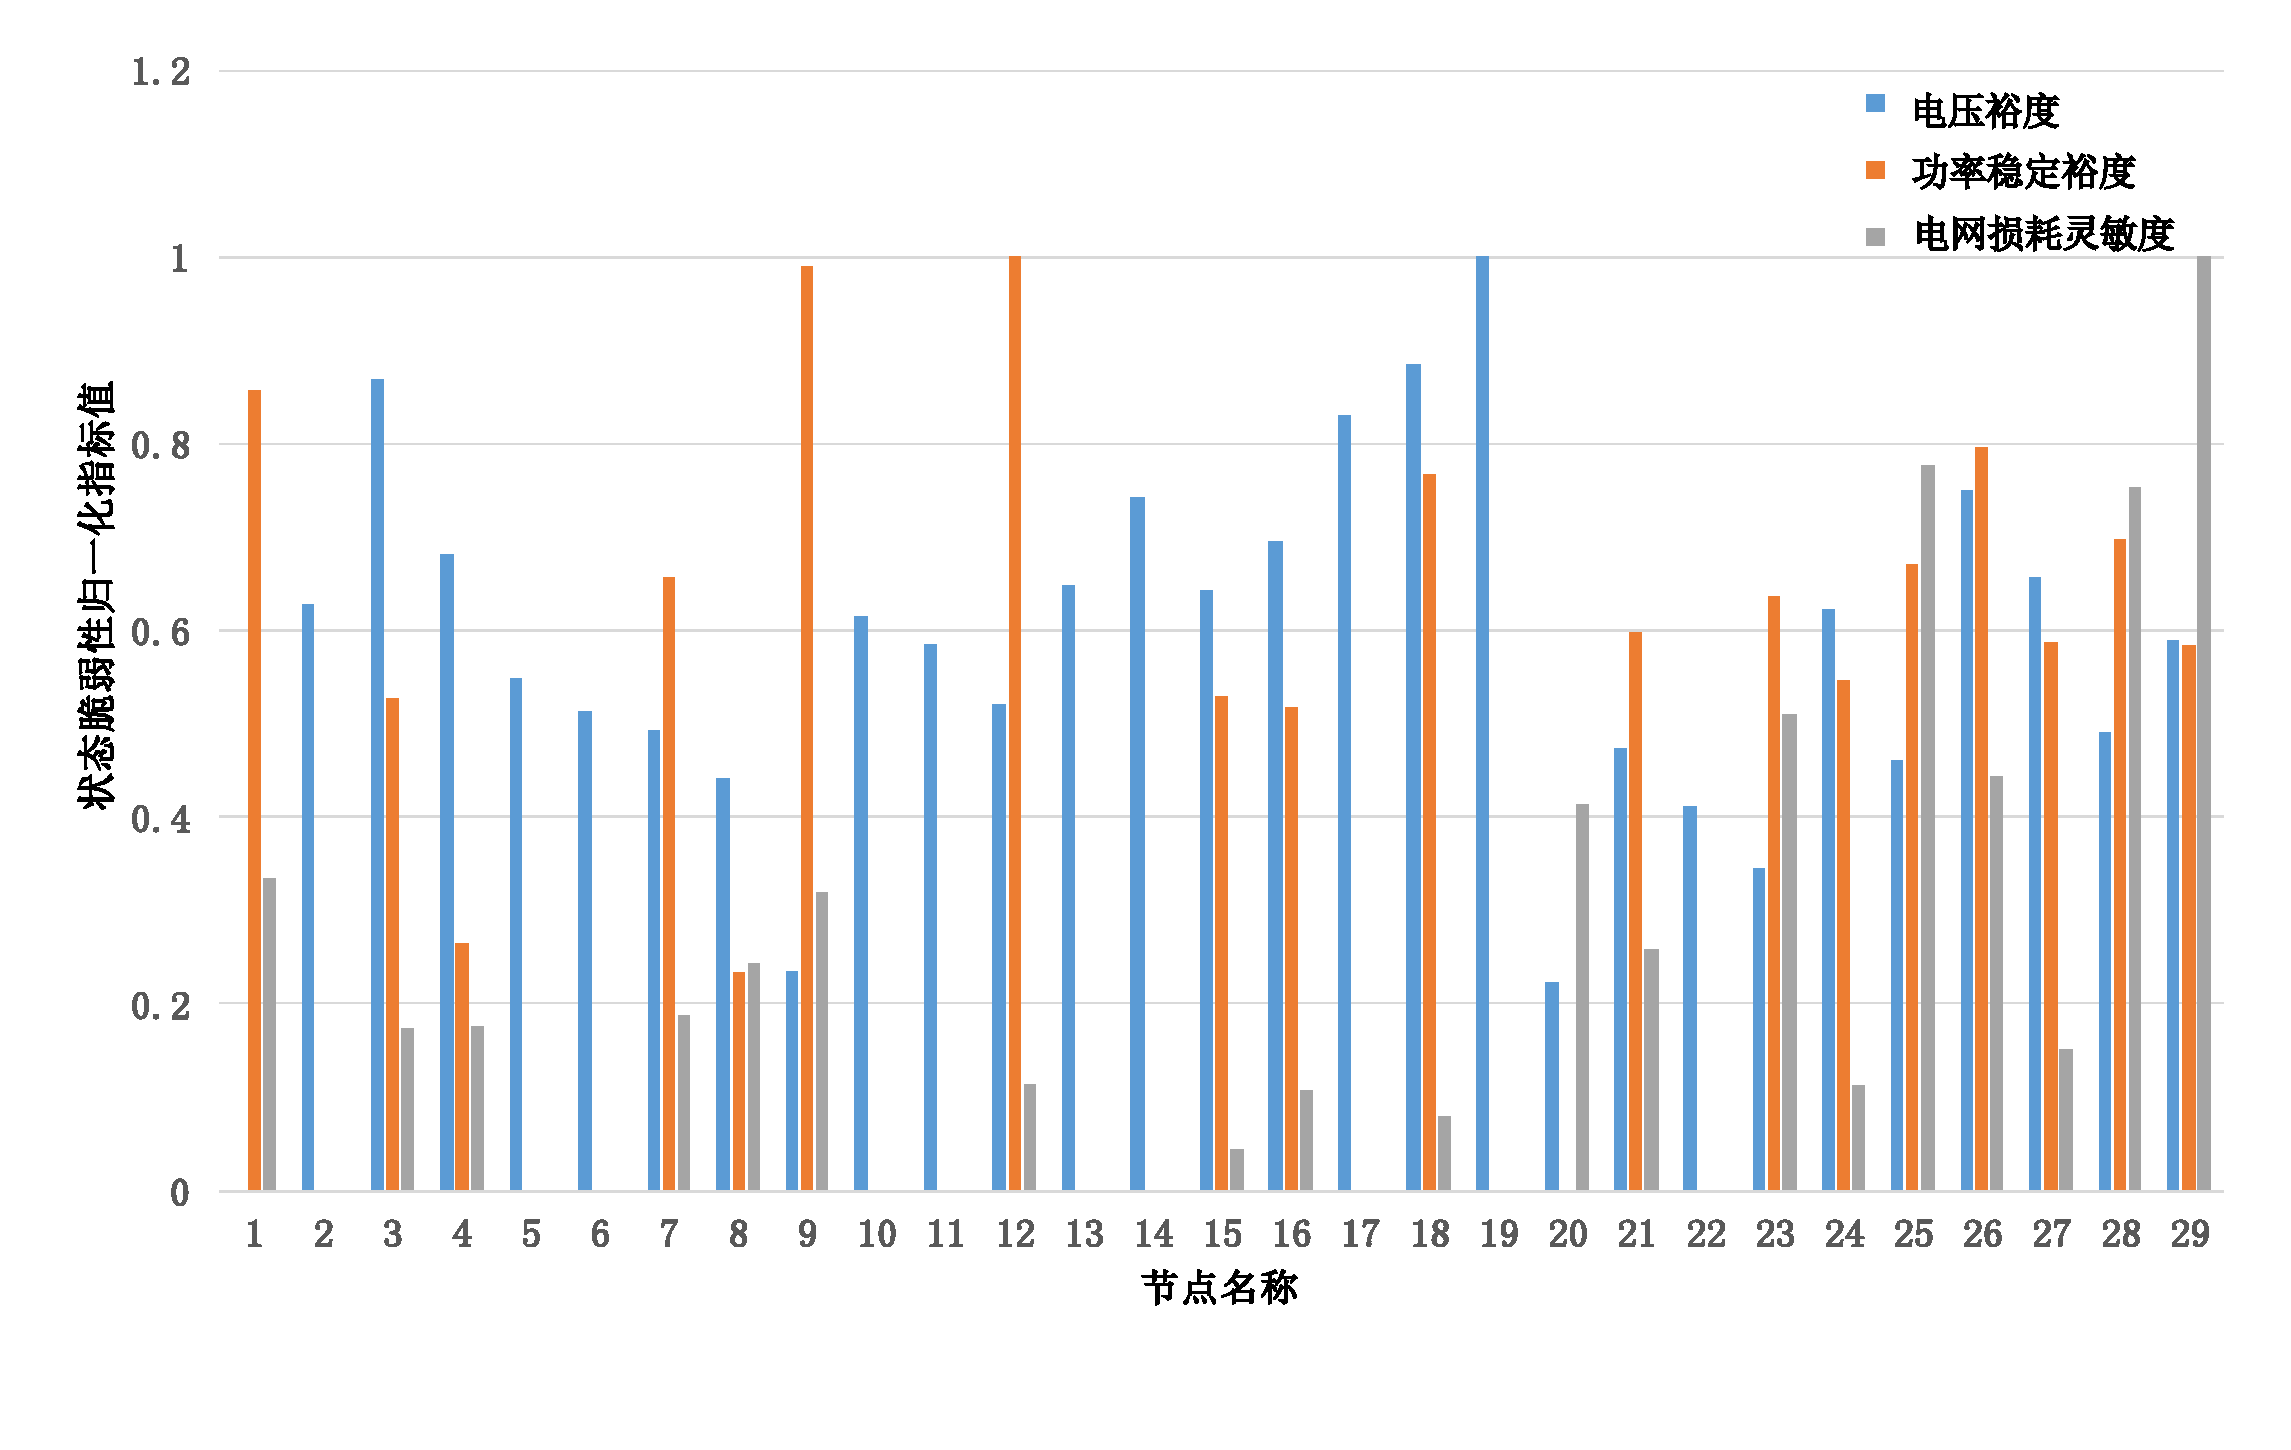
\includegraphics[width=14cm,height=8.1cm]{state_3index.pdf}
  \caption{$IEEE39$节点各状态脆弱性指标}
  \label{fig:state_3index}
\end{figure}
值得注意的是,电压裕度指标和功率稳定裕度指标为“成本型”指标,其值越大意味着节点的脆弱程度越小,而本文采用的是“效益型”指标,为统一指标类型,不改变指标的定义与概念,清晰描述系统节点的脆弱程度,
表\ref{tab:chap5:Index2_frabric39}为电压裕度和功率稳定裕度指标进行数值反向的实验结果,指标值越大,表示其电压裕度和功率稳定裕度越小,节点的脆弱程度越高。

节点2、5、6、10、11、13、14、17、19和22为联络节点,其注入有功功率和无功功率都等于零,所以其负荷模型的数据为0,因此,在功率稳定裕度指标和电网损耗灵敏度指标中,将这些节点的指标数值设置为0。
从表\ref{tab:chap5:Index2_frabric39}和图\ref{fig:state_3index}可知,在$IEEE39$系统中,电压裕度指标值最大的为节点19,其次是节点18、3、17、14、26、16和4,这些节点的电压波动性较大,其电压
稳定性差,对于电网负荷变化较为敏感,就从电压裕度指标而言,节点脆弱程度较高,原因在于这些节点处于中心位置,在功率负荷变化情况下,距离发电节点较远,传输线路较长,输电能力较弱,其线路压降和损耗
较大,从而导致电压波动较大。电压裕度指标值较小的为节点1、20、9、23、22、8、25,其中节点20、23、22和25分别与发电节点34、36、35和37直接连接,节点1和9与发电节点39相连,节点8和21距离发电节点
较近,结合系统结构示意图\ref{fig:fabric_39},一般距离发电节点较近的负荷节点,电能传输距离较短,线路损耗较小,传输效率高,因此节点的电压值波动小,其脆弱性较小;
功率稳定裕度指标值最大的为节点9,其次较大的节点为12、1、26、18、28、25,从附录A中的$IEEE39$负荷节点数据可以看出,这些节点的有功功率的额定容量较小,这意味着节点承受过负荷的能力较小,
节点的脆弱性较高。而节点20、8、4、16、3、15的指标值较小,节点的有功功率额定容量较大,其过负荷能力较强,节点脆弱程度低;
电网损耗灵敏度指标值最大的为节点29,其次为节点25、28、23、26、20,这些节点在负荷增加时,所引起电网损耗较大,根据$IEEE39$系统结构示意图可以看出,相较于其他节点,这些节点大都连接或距离发电
节点较近,在电能传输中起到了关键作用,当节点功率负荷增加时,会很大程度影响到电网的潮流分布,进而使电网整体损耗增大,所以这些节点的脆弱程度较大。指标值较小的节点有15、18、16、24、12,
这些节点偏离发电节点,其负荷变化对电网整体损耗影响较小,节点脆弱性较小。


根据权重向量计算得到的系统状态脆弱性指标结果如图~\ref{fig:state_39}~所示。
\begin{figure}[H] % use float package if you want it here
  \centering
  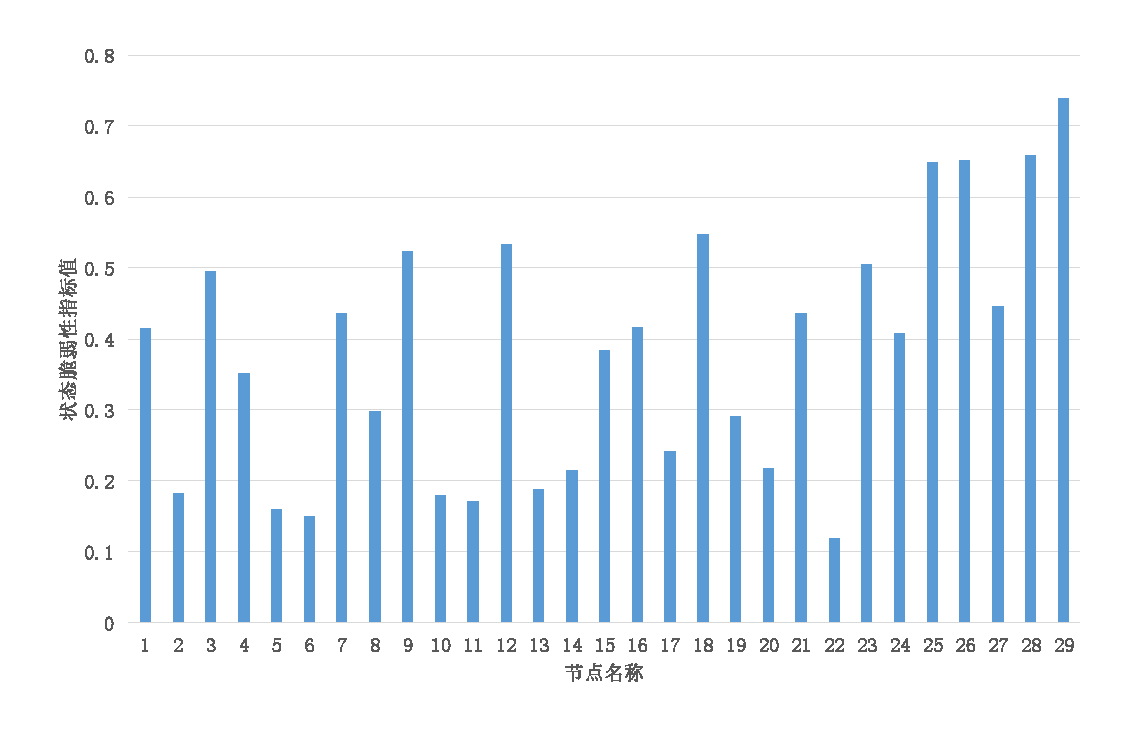
\includegraphics[width=14cm,height=8.64cm]{state_39.pdf}
  \caption{$IEEE39$状态综合脆弱性指标}
  \label{fig:state_39}
\end{figure}
从图\ref{fig:state_39}可知,节点29、28、26、25、18、12、9、3、1、7、16的状态综合脆弱性指标值较大,有些节点在电压值稳定性方面表现较差,电压波动较大,比如节点3、16、18,在节点的过负荷能力方面,
承担电网负荷的能力较差,比如节点1、12、26、25、28、18,在电网损耗方面,节点29、25、28、26对系统的影响较大。因此,系统节点对于电网运行状态的影响时多方面的,其影响表现在一个或多个方面,是多方面
指标因素综合影响的结果。从权重向量来看,功率稳定裕度指标占分配比重较大,所以在状态评估结果上,其脆弱节点在数量上占据优势。

通过上述状态脆弱性实验分析可得出,距离发电节点越远的节点,电能传输能力较弱,电压波动较大,节点负荷容量较小的节点其承受过负荷的能力较弱,功率稳定裕度小,在电能传输过程中处于中枢位置的节点,
在负荷变化时,所以引起的电网损耗较大。以上这些节点的状态脆弱性较强。

\subsection{电网综合脆弱性分析}
\label{sec:singleAnalysis}
根据D-S证据理论融合结构和状态两个指标得到$IEEE39$系统脆弱性综合评价指标结果,如图\ref{fig:stric_state}所示。
\begin{figure}[H] % use float package if you want it here
  \centering
  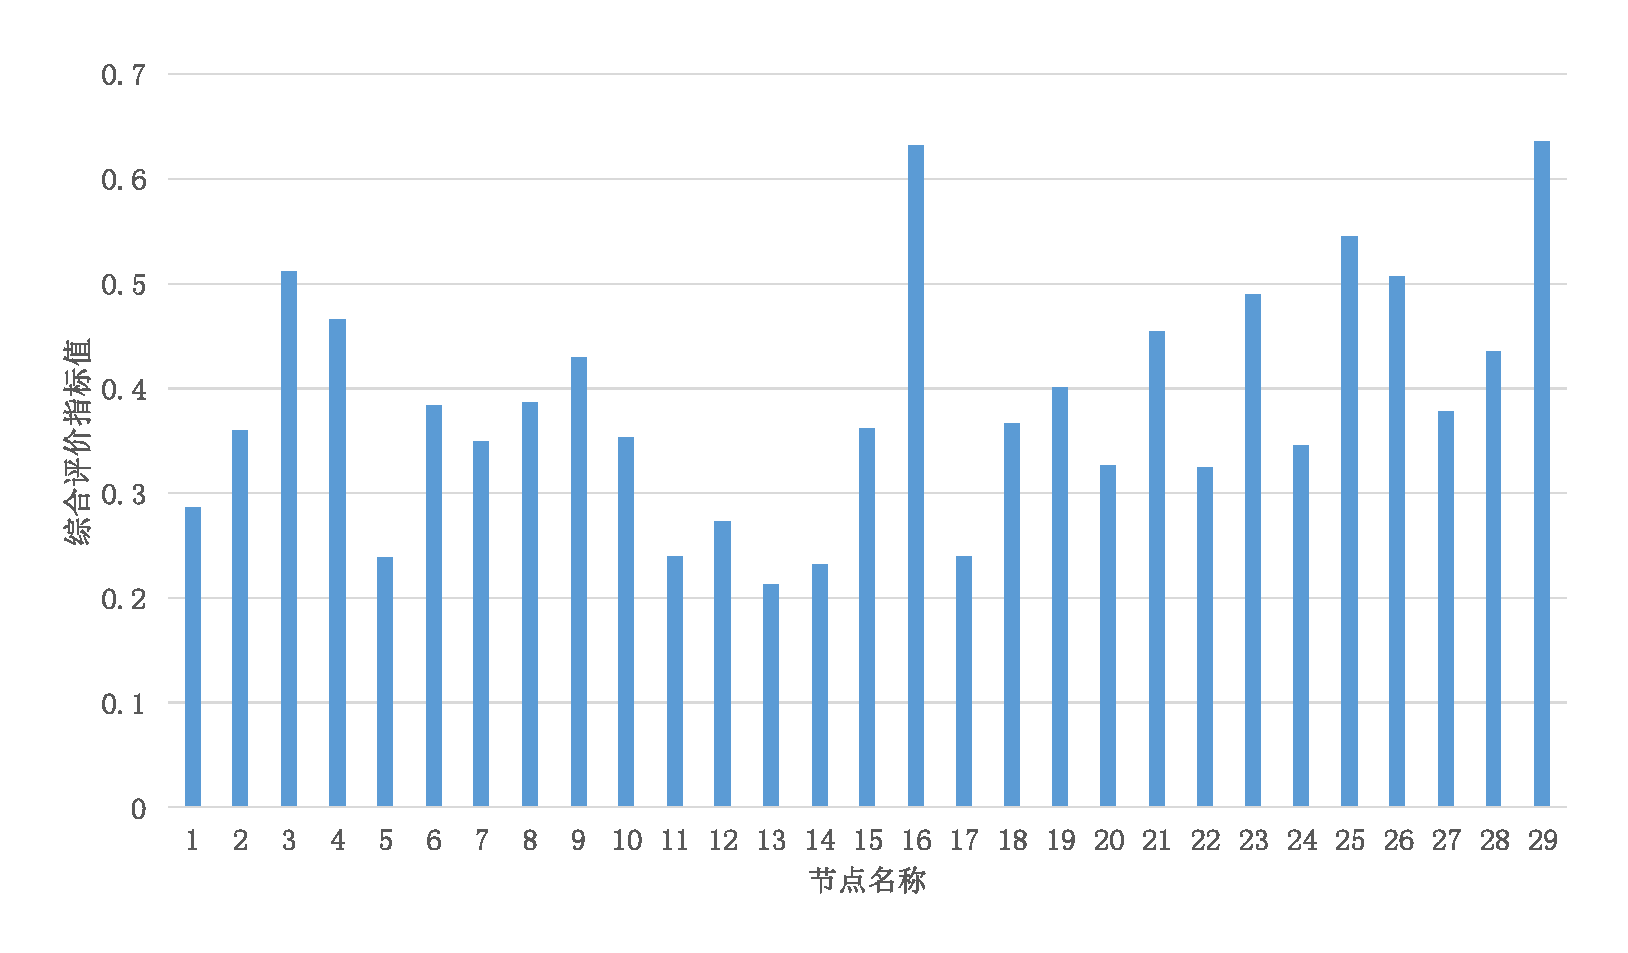
\includegraphics[width=14cm,height=8.64cm]{stric_state.pdf}
  \caption{$IEEE39$脆弱性综合评价指标}
  \label{fig:stric_state}
\end{figure}

从图\ref{fig:stric_state}可以看出,节点16、29、25、3、26、23、4、21的脆弱性综合评价指标值较大,节点脆弱性强,结合结构脆弱性和状态脆弱性两方面来看,这些节点的结构脆弱性综合指标和状态脆弱性
综合指标值数值相对较大,且数值大小差别不大,在进行数据融合时,结构和状态脆弱性指标作为两条独立的证据,两者之间的契合性较强,所得到的脆弱性综合评价指标值相对较大。另外,这些节点在脆弱性二级指标
下所占的比重大小也是影响其综合脆弱性的重要原因,比如节点16在结构脆弱性的三项指标中的脆弱性表现很好,其电气度、电气介数和$PageRank$值分别为0.7、1和0.78,在状态脆弱性指标方面,其电压裕度指标值
为0.695,虽然其功率稳定裕度指标值和电网损耗灵敏度指标值方面脆弱性表现较差,但这并不影响其在综合脆弱性评价值结果上的脆弱性表现,除此之外,就结构脆弱性指标方面,在电气度指标下脆弱性表现较好的有
节点29,电气介数指标下表现较好的有节点29、25、3、23、21,$PageRank$值指标下表现较好的有节点3、4,其他节点在上述结构指标下表现中庸或较差;状态脆弱性指标下,电压裕度指标方面表现较好的有节点3、
26、4,功率稳定裕度指标方面表现较好的有节点25、26、23、21,电压损耗灵敏度方面表现较好的有节点25、23,其他节点在上述状态指标下表现中庸或较差;从这一方面可以说明,在进行电网脆弱性评估上,要从
多方面考虑系统的评价指标,确保得到科学、全面的综合评价结果。

节点12、13、5、14、11、17、1的脆弱性综合评价指标值较小,节点脆弱性较弱,节点脆弱程度较小,这些节点在结构和状态指标值大小差别很大,两证据之间的契合性较差,另外的原因在于这些指标在绝大部分指标下
的脆弱性表现较差,从而导致系统综合评价结果的脆弱性表现较差,比如节点12,其三个结构指标下的脆弱性表现均比较差,其电气度、电气介数和$PageRank$指标值分别为0、0和0.05,在状态脆弱性指标方面,虽然其
在功率稳定裕度指标方面表现较好,其指标值达到了0.987,但在另外两个状态指标下的脆弱性表现较差,所以其综合脆弱性评价结果较小。

通过综合脆弱性指标结果可以得到,结构和状态脆弱性表现均比较强的节点,在证据融合时,二者契合性较强,节点的综合脆弱程度较强。

%节点29在电气介数、$PageRank$值和电网损耗灵敏度方面表现较好,电压裕度指标和功率稳定裕度指标表现中庸,电气度指标表现较差



\section{电网脆弱性等级评估}
\label{sec:multiAssessment}
根据上一节的$IEEE39$系统的脆弱性评价指标值,从系统节点的指标值分布和综合评价指标值两个方面考虑,分别基于聚类和综合指标排序方法确定和评估$IEEE39$系统节点的脆弱性等级,从而确定系统各节点的
脆弱程度。

\subsection{基于聚类算法的电网节点脆弱性等级评估}
\label{sec:K_means1}

聚类算法是机器学习领域中无监督学习中的一类算法,在"无监督学习"中,训练样本的标记信息是未知的,目标是通过对无标记训练样本的学习来揭示数据的内在性质及规律,为进一步的数据分析提供基础\cite{refs82}。
在聚类算法中,主要分为原型聚类、密度聚类和层次聚类,原型聚类中分为k均值($k-means$)聚类、学习向量量化(LVQ)聚类和高斯混合聚类,密度聚类中有DBSCAN聚类,层次聚类中有AGNES聚类。

在$IEEE39$系统节点脆弱性指标评估结果中,采用结构综合脆弱性指标和状态综合脆弱性指标作为系统脆弱性评估结果的特征,由于本文的脆弱性研究对象的特征较为简单且节点所对应的数据量不大,因此,在常用的
聚类算法中选择$k-means$聚类算法进行系统节点脆弱性等级评定。

$k-means$聚类算法原理较为简单,实现比较容易,收敛速度快,并且在参数调整上,只需要调整簇数$k$即可。其算法流程如下:

$(1)$首先确定$k$值,即期望将数据集经过聚类得到$k$个集合;

$(2)$从随机初始化$k$个中心点作为质心;

$(3)$对数据集中每一个点,计算其与每个质心的距离(欧式距离),将数据点划分到距离所属质心点近的集合中;

$(4)$将所有数据划分好后,基于这些分类点取每一类中向量的均值重新计算每个集合的质心;

$(5)$如果新计算出来的质心和原来的质心之间的距离小于某一个设置的阈值(表示重新计算的质心的位置变化不大,趋于稳定,或者说收敛),可以认为聚类已经达到期望的结果,算法终止;
若新质心和原质心之间距离差很大,需要迭代3~5步骤。

下面对$IEEE39$系统的结构和状态综合脆弱性指标进行聚类分析,聚类结果如图\ref{fig:K_means}、表\ref{tab:k_means}所示。
\begin{figure}[H] % use float package if you want it here
  \centering
  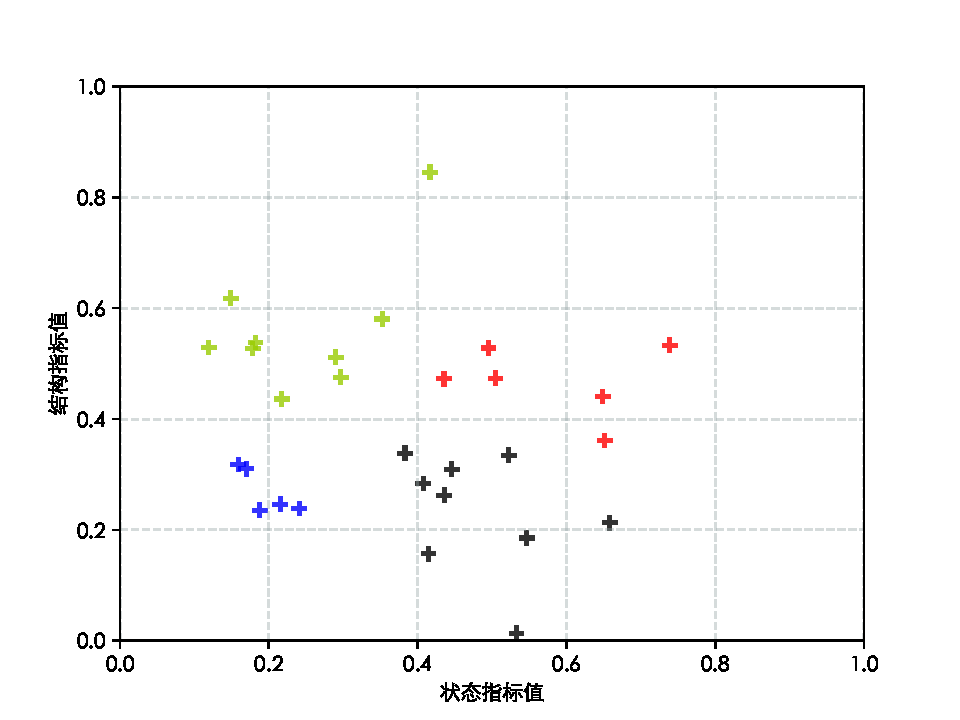
\includegraphics[width=12cm,height=8.965cm]{K_means.pdf}
  \caption{$IEEE39$脆弱性指标聚类结果图}
  \label{fig:K_means}
\end{figure}

\begin{table}[H]
  \centering
  \caption{$IEEE39$系统脆弱性指标值聚类结果表}
  \label{tab:k_means}
  \begin{tabular}{C{1.5cm}C{2.25cm}C{1.5cm}C{7.25cm}}
  \toprule
  \textbf{所属类别} & \textbf{质心坐标} & \textbf{节点颜色} & \textbf{节点名称}  \\
  \midrule
  0             &(0.5\ ,\ 0.246)       & 绿色        & 1、7、9、12、15、18、24、26、27、28  \\
  1             &(0.201\ ,\ 0.415)     & 红色        & 2、5、6、8、10、11、13、14、17、19、20、22 \\ 
  2             &(0.513\ ,\ 0.553)     & 蓝色        & 3、4、16、21、23、25、29 \\ 
  \bottomrule
  \end{tabular}
\end{table}

从图\ref{fig:K_means}中结构和状态脆弱性综合指标值的数据点分布情况来看,所属类别为0的绿色数据点在状态脆弱性综合指标上所占的比重较大,其对应节点偏向于状态脆弱性,如节点26、28、12、18,这些节点
在电压稳定性、过负荷能力以及电网损耗方面表现较差,其状态脆弱程度较大;所属类别为1的红色数据点在结构脆弱性综合指标上所占比重相对较大,其对应节点偏向于结构脆弱性,如节点2、6、10、19,这些节点在电网
结构联通和能量传输中起至关重要的作用,故其结构脆弱程度较大,在类别1的数据点中,节点5、11、12、13、17的结构和状态脆弱性指标均较小,在电力系统中的重要程度相对较小,故认为这些节点不脆弱;所属类别为2
的蓝色数据点其结构和状态脆弱性指标值均较大,说明这些节点在电网结构的重要程度以及运行状态下的脆弱程度较大,因此可将这些作为脆弱环节加以防范,其脆弱程度最大。

复杂网络理论认为结构决定功能,电力系统的拓扑结构是电能传输和系统正常运行的基础,当电网结构遭到破坏时,将会对电网的运行状态造成不可逆的影响。故本文认为节点的结构指标相对于状态指标重要程度高。
通过以上分析,可从指标分布情况下对各系统节点进行脆弱性等级评估,评估情况如表\ref{tab:k_means1}所示。
\begin{table}[H]
  \centering
  \caption{基于聚类的$IEEE39$系统脆弱性等级评估表}
  \label{tab:k_means1}
  \begin{tabular}{C{1.5cm}C{5cm}C{6cm}}
  \toprule
  \textbf{脆弱等级} & \textbf{等级描述} & \textbf{节点名称}  \\
  \midrule
  1 & 重要节点,脆弱性强 & 3、4、16、21、23、25、29 \\ 
  2 & 结构脆弱节点 & 5、8、11、13、14、17、20、22  \\
  3 & 状态脆弱节点 & 1、7、9、12、15、18、24、26、27、28\\ 
  4 & 非重要节点,脆弱性差 & 2、6、10、19 \\ 
  \bottomrule
  \end{tabular}
\end{table}


\subsection{基于综合指标排序的电网节点脆弱性等级评估}
在上一节中,通过指标融合方法得到节点的结构和状态脆弱性指标后,分别研究分析了系统节点结构脆弱性和状态脆弱性,再根据D-S证据理论对结构和状态指标融合得到节点综合评价指标结果,并进一步通过脆弱性
综合分析,识别出系统的脆弱环节。

本节基于脆弱性综合评价指标值对节点的脆弱程度评估并进行归一化,其节点脆弱性排序结果如图\ref{fig:nodeRank}所示。

\label{sec:multiAnalysis}
\begin{figure}[H] % use float package if you want it here
  \centering
  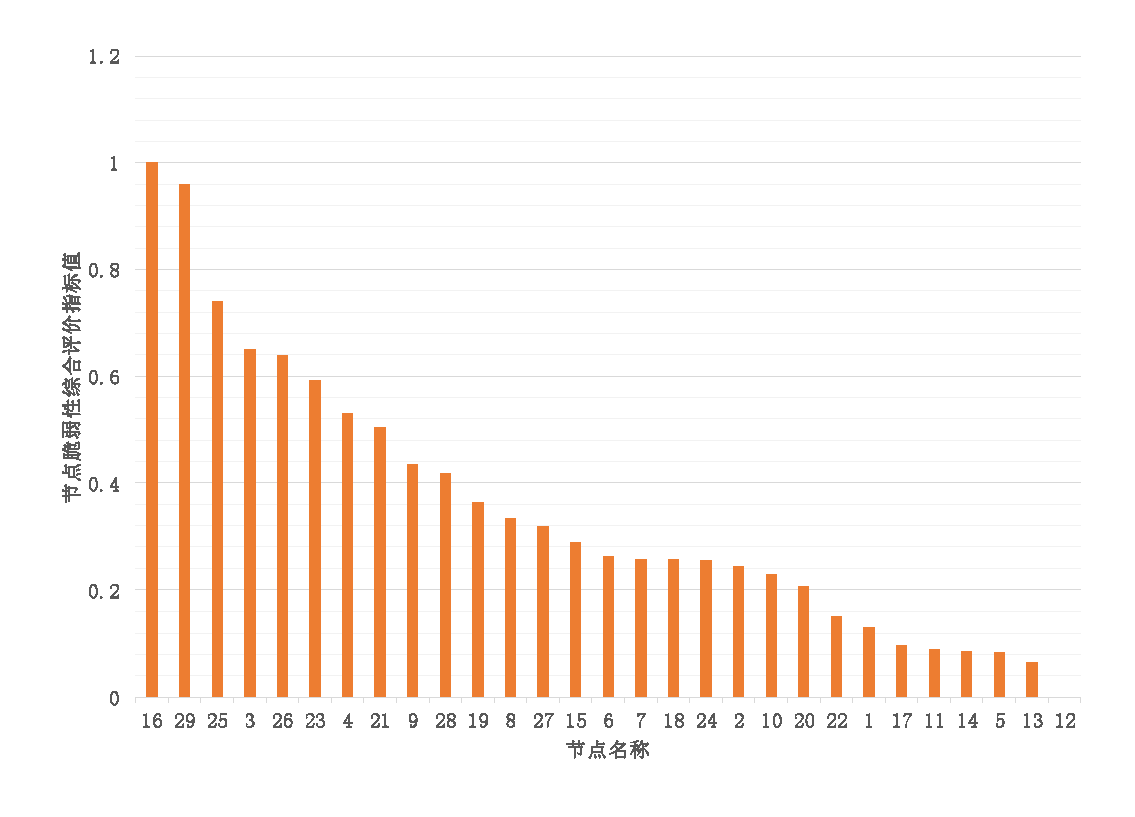
\includegraphics[width=14cm,height=9.62cm]{nodeRank.pdf}
  \caption{$IEEE39$综合脆弱性评价指标值排序图}
  \label{fig:nodeRank}
\end{figure}
本文根据$IEEE39$节点脆弱性综合评价指标值的分布特点,规定节点脆弱性综合评价指标值为0.6—1之间的节点为一级脆弱节点;0.3—0.6之间的节点为二级脆弱节点;0.3—0.2之间的节点为三级脆弱节点;低于0.2
的节点为四级脆弱节点。根据以上规则,节点等级评估情况如表\ref{tab:nodeRank}所示。
\begin{table}[H]
  \centering
  \caption{基于综合评价指标值的$IEEE39$系统脆弱性等级评估表}
  \label{tab:nodeRank}
  \begin{tabular}{C{1.5cm}C{5cm}C{6cm}}
  \toprule
  \textbf{脆弱等级} & \textbf{等级描述} & \textbf{节点名称}  \\
  \midrule
  1 & 重要节点,脆弱性强 & 16、29、25、3、26 \\ 
  2 & 脆弱节点,比较脆弱 & 23、4、21、9、28、19、8、27 \\
  3 & 脆弱节点,一般脆弱 & 15、6、7、18、24、2、10、20 \\ 
  4 & 非重要节点,脆弱性差 & 22、1、17、11、14、5、13、12 \\ 
  \bottomrule
  \end{tabular}
\end{table}


\subsection{结果分析与比较}
在以上脆弱性等级评估方法中,基于聚类方法得到的节点脆弱性等级评估结果,通过结构和状态指标值的分布情况来揭示数据值之间的内在规律,可以从结构和状态两个方面识别出系统脆弱环节,对故障防范、
系统结构规划具有积极意义;基于综合指标排序的节点脆弱性等级评估,通过综合指标结果来识别系统的脆弱环节,主要是从系统宏观角度全面评价系统节点的脆弱程度,这对于优化电网结构和整体负荷调度
具有很强的现实意义。



\section{本章小结}
\label{sec:sum5}

本章以$IEEE39$系统为研究对象,采用第四章节所建立的电网脆弱性综合评估模型进行系统节点的脆弱性分析,得到各系统节点的结构和状态脆弱性指标值,
分别分析各系统节点的结构脆弱性和状态脆弱性,实验表明,在结构脆弱性分析结果方面,节点的传输能力越大,所处位置的重要性越高,即节点所连支路越多,其结构脆弱性越强;在状态脆弱性分析结果方面,
距离发电节点较远、负荷容量较小、在电能传输过程中处于中枢位置的节点,在电压稳定性、过负荷能力及电网损耗方面表现较差,节点的状态脆弱性较强。

根据电网综合评估指标值,对系统节点综合脆弱性进行分析,实验分析表明,结构和状态脆弱性表现均比较强的节点,在证据融合时,二者契合性较强,节点的综合脆弱程度较强。通过研究结构参数和系统数据
证实了电网脆弱性综合评估模型的合理性与科学性。
最后,通过聚类算法和脆弱性综合评估结果对系统节点脆弱性等级评估,识别系统的脆弱环节,对后续系统的结构设计和加强关键环节的保护措施具有现实意义。


\chapter{总结与展望}
\label{cha:summery}

\section{全文总结}
\label{sec:sum}
电力系统作为维持经济和社会发展的重要组成部分,其对于国家发展的重要性不言而喻。电网脆弱性已成为越来越多专家学者研究的热门领域,为此本文针对电力系统中脆弱性现象给出了科学合理的定义与数学描述,
从电网的结构和状态两个方面提出脆弱性评估指标,并采用并改进指标融合方法建立了脆弱性量化评估模型,对电力系统进行脆弱性分析与量化评估,识别电力系统系统的脆弱环节,这对于设计
优化电网结构、降低电网大停电事故发生的概率等方面具有现实意义。全文的主要工作总结如下:

(1)通过查阅相关的文献资料,对电力系统脆弱性的发展及研究方法进行了综述。基于复杂网络理论验证分析了电力系统模型的小世界性和无标度性,通过研究复杂网络中局部与整体的关系,明确了本文
研究的关键问题。

(2)通过研究复杂系统脆弱性概念和电网脆弱性特征,得到了电力系统的脆弱性本质在于其对内、外扰动的耐受程度,并从结构和状态两个方面研究电力系统脆弱性,进而得出一个较为清晰全面的
系统脆弱性概念。

(3)根据对电力系统脆弱性的定义,在结构脆弱性方面,在扰动作用下,其侧重于电网结构保持完整性的能力和系统受影响的程度,基于复杂网络理论对电网系统进行建模,并提出结构脆弱性指标;
在状态脆弱性方面,本文在电压稳定性、承受负荷能力和电网损耗方面分别提出状态脆弱性指标,并建立随机负荷模型,结合潮流计算采用蒙特卡洛模拟实验方法计算分析电网的运行状态指标。

(4)针对提出的结构和状态方面的二级脆弱性指标,选择合适的数学方法对其进行无量纲归一化处理,然后采用改进熵权法和离差最大化法分别对结构和状态指标集进行权重分配,并得到结构和状态综合脆弱性指标,
最后采用D-S证据理论对结构和状态一级脆弱性指标进行融合得到系统综合脆弱性评价指标,形成了电力系统综合评估模型。

(5)以$IEEE39$标准系统为例,依据本文所建立的电力系统脆弱性综合评估模型,使用MATLAB工具进行仿真实验,结合电网结构和系统状态参数,分别研究分析了系统结构
和状态脆弱性并进行电网综合脆弱性分析,最后,通过电网脆弱性综合评估结果对系统节点的脆弱程度进行了等级评估,识别出系统脆弱环节。

\section{未来工作展望}
\label{sec:feature}
由于本人水平与时间所限,对于电力系统的脆弱性分析与研究还存在需要完善及深入探讨之处,后续的工作可以从以下几个方面展开:

(1)由于电网模型所限,本文在发电节点方面的脆弱性分析针对的只是结构方面,状态脆弱性指标只针对负荷节点,因为对于电网状态脆弱性是基于负荷变化进行研究的,而在潮流计算中发电节点为$PV$节点,
即发电节点的电压是不变的且有功功率为0,所以无法用本文定义的状态脆弱性指标来量化,后续可以采用其他电网模型通过暂态分析研究系统的状态脆弱性。

(2)本文在电网脆弱性研究方面,针对的只是系统节点,所以在识别系统脆弱环节方面,将节点的脆弱程度作为本文的研究重点,虽然电气介数指标考虑了支路对于节点的影响,但并未单独考虑系统支路对于
电力系统的影响,后续可以综合节点和支路两方面研究分析电网脆弱性。

(3)由于实验条件和时间的有限,本文中通过查阅文献的方式最终用概率统计的方式建立了随机性负荷概率模型来模拟实际负荷变化。若实验条件许可,可以对实际的电力系统所在地负荷需求进行采样统计,
得到日变化或年变化的真实数据再用本文所建立的模型进行系统的脆弱性量化分析,这样得到的评价结果更具现实意义。

%%% 其它部分
\backmatter

% 致谢
\begin{acknowledgement}
在此论文成稿之际,谨向我尊敬的导师苏永清副教授致以最诚挚的感谢!本文的选题内容、研究思路与分析过程均在苏老师的悉心指导下完成。
在两年的课题研究过程中,始终得到苏老师科研上的帮助与指导。苏老师渊博的学识、严谨的治学理念以及以身作则的工作态度,深深地感染
了我,在此我谨向您致以深切的感谢与诚挚的敬意。感谢岳继光教授与董延超副教授在工程项目及日常生活中给予我的帮助。你们严谨的学术
态度与踏实的工作作风为实验室建立了严谨求实的研究氛围,感谢你们为实验室的辛勤付出。

感谢同门师兄张鲲鹏与陈峰在研究课题中的指导,感谢刘志刚与徐晨剑师兄在工程项目中对我的帮助,徐晨剑师兄的论文~\LaTeX~模板使我受
益匪浅。感谢侯培鑫博士在学术方法上对我的提点以及多次赠书之情,感谢王森博博士与王栗博士在项目中的指导与帮助,祝你们顺利毕业。
感谢同届研究生施梁、汪嬴、唐丹旭、吴琛浩,同窗之情,友谊长存,祝你们今后工作顺利。感谢刘雪娇与穆慧华两位师妹在~502~研究所与
~811~研究所工程项目中的协助。感谢同济大学先进测控技术课题组徐刚、陈策、乔琪、张爽、武新然、李炅聪等全体成员,伴我度过了难忘的
研究生时光,在此祝大家前程似锦,幸福快乐。

同时感谢张志明老师对我在虚拟仪器俱乐部工作的支持与帮助,感谢黄蓉荣师姐、吉方成师兄与陈阳师兄在虚拟仪器俱乐部对我的指导与帮助,
祝同济大学虚拟仪器俱乐部越办越好。感谢贾青老师与同济大学~PACE~中心对我工作上的支持,感谢张世博师兄在~Urban Flexible Vehicle~项目
中的帮助,那些熬夜调车的夜晚至今历历在目。

此外,感谢好友狄宗林与邵瑶夏,与你们相识让我看到青年才俊们的努力与拼搏,祝你们最终实现梦想。感谢好友~Paolo Curti~在意大利的
热情招待,Omegna~湖畔的烟花绚烂依旧。


最后,要感谢我的父亲母亲,是你们的支持才使我能走到今天。养育之恩,无以为报,你们健康快乐是我最大的心愿。在未来的学习、
工作与生活中,我会继续锐意进取,成于精勤、止于至善。


~~\\


\rightline{赵闻达\qquad \quad}

\rightline{2018年3月于上海嘉定}
\end{acknowledgement}

% 参考文献
\printTJbibliography

% 附录
\begin{appendix}
\chapter{$IEEE39$系统数据}
\label{cha:engorg0}

\section{$IEEE$39系统节点}
\label{sec:lp0}

\begin{table}[H]
  \centering
  \caption{$IEEE$39系统发电节点}
  \label{tab:chap5:generator39}
    \begin{tabular}{C{3cm}C{3cm}C{3cm}}
\toprule
\textbf{节点名}        &\textbf{额定有功功率($MW$)}      &\textbf{是否为平衡节点}         \\
\midrule
            30        &250 &否\\
            31        &677.81 &是 \\
            32        &650  &否 \\
            33        &632  &否 \\
            34        &508   &否\\
            35        &650 &否\\
            36        &560 &否\\
            37        &540 &否\\
            38        &830 &否\\
            39        &1000 &否\\
\bottomrule
\end{tabular}
\end{table}

\begin{table}[H]
  \centering
  \caption{$IEEE$39系统负荷节点}
  \label{tab:chap5:load39}
    \begin{tabular}{C{1.2cm}C{2.4cm}C{2.4cm}C{1.2cm}C{2.4cm}C{2.4cm}}
\toprule
            \textbf{节点名}        &\textbf{额定有功功率($MW$)}      &\textbf{额定无功功率($MVar$)}   & \textbf{节点名}        &\textbf{额定有功功率($MW$)}      &\textbf{额定无功功率($MVar$)}       \\
\midrule
            1        &97.6 &44.2 & 16        &329.0 &32.3\\
            2        &0.0 &0.0 &17        &0.0 &0.0\\
            3        &322.0  &2.4 &18        &158.0 &30.0\\
            4        &500.0  &184.0 &19        &0.0 &0.0\\
            5        &0.0 &0.0 &20        &680.0 &103.0\\
            6       &0.0 &0.0 &21        &274.0 &115.0\\
            7        &233.8 &84.0 &22        &0.0 &0.0\\
            8        &522.0 &176.6 &23        &247.5 &84.6\\
            9        &6.5 &-66.6 &24        &308.6 &-92.2\\
            10        &0.0 &0.0 &25        &224 &47.2\\
            11        &0.0 &0.0 &26        &139 &17\\
            12        &8.53 &88.0 &27        &281 &75.5\\
            13        &0.0 &0.0 &28        &206 &27.6\\
            14        &0.0 &0.0 &29        &283.5 &26.9\\
            15        &320.0 &153.0 & & &\\
\bottomrule
\end{tabular}
\end{table}

\chapter{$IEEE118$系统数据}
\label{cha:engorg}

\section{$IEEE$118系统发电节点}
\label{sec:lp}

\begin{table}[H]
\centering
\caption{$IEEE$118系统发电节点}
\label{tab:chap5:generator118}
\begin{tabular}{C{1.4cm}C{2.4cm}C{2.2cm}C{1.4cm}C{2.4cm}C{2.2cm}}
\toprule
\textbf{节点名} & \textbf{额定有功功率(MW)} & \textbf{ 是否是平衡节点 } & \textbf{节点名} & \textbf{额定有功功率(MW)}  & \textbf{ 是否是平衡节点 } \\
\midrule
1   & 0          & 否       & 65  & 391        & 否       \\
4   & 0          & 否       & 66  & 392        & 否       \\
6   & 0          & 否       & 69  & 516.4      & 是       \\
8   & 0          & 否       & 70  & 0          & 否       \\
10  & 450        & 否       & 72  & 0          & 否       \\
12  & 85         & 否       & 73  & 0          & 否       \\
15  & 0          & 否       & 74  & 0          & 否       \\
18  & 0          & 否       & 76  & 0          & 否       \\
19  & 0          & 否       & 77  & 0          & 否       \\
24  & 0          & 否       & 80  & 477        & 否       \\
25  & 220        & 否       & 85  & 0          & 否       \\
26  & 314        & 否       & 87  & 4          & 否       \\
27  & 0          & 否       & 89  & 607        & 否       \\
31  & 7          & 否       & 90  & 0          & 否       \\
32  & 0          & 否       & 91  & 0          & 否       \\
34  & 0          & 否       & 92  & 0          & 否       \\
36  & 0          & 否       & 99  & 0          & 否       \\
40  & 0          & 否       & 100 & 252        & 否       \\
42  & 0          & 否       & 103 & 40         & 否       \\
46  & 19         & 否       & 104 & 0          & 否       \\
49  & 204        & 否       & 105 & 0          & 否       \\
54  & 48         & 否       & 107 & 0          & 否       \\
55  & 0          & 否       & 110 & 0          & 否       \\
56  & 0          & 否       & 111 & 36         & 否       \\
59  & 155        & 否       & 112 & 0          & 否       \\
61  & 160        & 否       & 113 & 0          & 否       \\
62  & 0          & 否       & 116 & 0          & 否     \\
\bottomrule
\end{tabular}
\end{table}

\section{$IEEE$118系统负荷节点}
\begin{table}[H]
   \centering
   \caption{$IEEE$118系统负荷节点}
   \label{tab:chap5:load118}
     \begin{tabular}{C{1.2cm}C{2.4cm}C{2.4cm}C{1.2cm}C{2.4cm}C{2.4cm}}
\toprule
 \textbf{节点名}        &\textbf{额定有功功率($MW$)}      &\textbf{额定无功功率($MVar$)}   & \textbf{节点名}        &\textbf{额定有功功率($MW$)}      &\textbf{额定无功功率($MVar$)}       \\
\midrule
2  & 20 & 9  & 57  & 12 & 3  \\
3  & 39 & 10 & 58  & 12 & 3  \\
5  & 0  & 0  & 60  & 78 & 3  \\
7  & 19 & 2  & 63  & 0  & 0  \\
9  & 0  & 0  & 64  & 0  & 0  \\
11 & 70 & 23 & 67  & 28 & 7  \\
13 & 34 & 16 & 68  & 0  & 0  \\
14 & 14 & 1  & 71  & 0  & 0  \\
16 & 25 & 10 & 75  & 47 & 11 \\
17 & 11 & 3  & 78  & 71 & 26 \\
20 & 18 & 3  & 79  & 39 & 32 \\
21 & 14 & 8  & 81  & 0  & 0  \\
22 & 10 & 5  & 82  & 54 & 27 \\
23 & 7  & 3  & 83  & 20 & 10 \\
28 & 17 & 7  & 84  & 11 & 7  \\
29 & 24 & 4  & 86  & 21 & 10 \\
30 & 0  & 0  & 88  & 48 & 10 \\
33 & 23 & 9  & 93  & 12 & 7  \\
35 & 33 & 9  & 94  & 30 & 16 \\
37 & 0  & 0  & 95  & 42 & 31 \\
38 & 0  & 0  & 96  & 38 & 15 \\
39 & 27 & 11 & 97  & 15 & 9  \\
41 & 37 & 10 & 98  & 34 & 8  \\
43 & 18 & 7  & 101 & 22 & 15 \\
44 & 16 & 8  & 102 & 5  & 3  \\
45 & 53 & 22 & 106 & 43 & 16 \\
47 & 34 & 0  & 108 & 2  & 1  \\
48 & 20 & 11 & 109 & 8  & 3  \\
50 & 17 & 4  & 114 & 8  & 3  \\
51 & 17 & 8  & 115 & 22 & 7  \\
52 & 18 & 5  & 117 & 20 & 8  \\
53 & 23 & 11 & 118 & 33 & 15 \\
\bottomrule
\end{tabular}
\end{table}

\end{appendix}


% 个人简历
\begin{resume}
\resumeitem{个人简历:}
\noindent 1995 年 3 月 1 日出生于山东省临沂市。\\
\noindent 2017 年 6 月本科毕业于山东科技大学获得学士学位。\\
\noindent 2017 年 9 月进入同济大学攻读硕士学位至今。


\resumeitem{参与项目:} % 有就写,没有就删除
\begin{enumerate}[{[}1{]}]
\item 国家重点研发计划“产品全生命周期模型管理技术与系统”项目
\item 航天基金“航天卫星电源系统性能分析”项目
\end{enumerate}

\end{resume}

\end{document}
